\RequirePackage{pdfmanagement-testphase}
\DeclareDocumentMetadata {lang=en-US}

% xmp metadata for pdf
% Originally used \usepackage[a-2a]{pdfx}
% \usepackage{hyperxmp} replaced it
% \RequirePackage{pdfmanagement-testphase} replaced it
% \PassOptionsToPackage{enable-debug,check-declarations}{expl3} broke with version 0.9 of tagpdf
% \ExplSyntaxOn no need for these 3 lines because metadata can handle it
% \pdfmanagement_add:nnn{Catalog}{Lang}{(enUS)} enUS is wrong, should be en-US
% \ExplSyntaxOff

\documentclass[11pt,
  english,
  a4paper,
]{article}
\usepackage{sa4ss}
\usepackage{amsmath,amssymb,array}
\usepackage{booktabs}

% From tagged-template.latex
\usepackage{lmodern}
\usepackage{ifxetex,ifluatex}
\ifnum 0\ifxetex 1\fi\ifluatex 1\fi=0 % if pdftex
  \usepackage[T1]{fontenc}
  \usepackage[utf8]{inputenc}
  \usepackage{textcomp} % provide euro and other symbols
\else % if luatex or xetex
  \usepackage{unicode-math}
  \defaultfontfeatures{Scale=MatchLowercase}
  \defaultfontfeatures[\rmfamily]{Ligatures=TeX,Scale=1}
\fi

% Use upquote if available, for straight quotes in verbatim environments
\IfFileExists{upquote.sty}{\usepackage{upquote}}{}
\IfFileExists{microtype.sty}{% use microtype if available
  \usepackage[]{microtype}
  \UseMicrotypeSet[protrusion]{basicmath} % disable protrusion for tt fonts
}{}
\makeatletter
\@ifundefined{KOMAClassName}{% if non-KOMA class
  \IfFileExists{parskip.sty}{%
    \usepackage{parskip}
  }{% else
    \setlength{\parindent}{0pt}
    \setlength{\parskip}{6pt plus 2pt minus 1pt}}
}{% if KOMA class
  \KOMAoptions{parskip=half}}
\makeatother
\usepackage{xcolor}
\IfFileExists{xurl.sty}{\usepackage{xurl}}{} % add URL line breaks if available
\hypersetup{
  pdftitle={Status of copper rockfish (Sebastes caurinus) in U.S. waters off the coast of Washington in 2021 using catch and length data},
  pdflang={en},
  hidelinks,
  pdfcreator={LaTeX via pandoc}}
\urlstyle{same} % disable monospaced font for URLs
\usepackage{longtable}
% Correct order of tables after \paragraph or \subparagraph
\usepackage{etoolbox}
\makeatletter
\patchcmd\longtable{\par}{\if@noskipsec\mbox{}\fi\par}{}{}
\makeatother
% Allow footnotes in longtable head/foot
\IfFileExists{footnotehyper.sty}{\usepackage{footnotehyper}}{\usepackage{footnote}}
\makesavenoteenv{longtable}
\usepackage{graphicx}
\makeatletter
\def\maxwidth{\ifdim\Gin@nat@width>\linewidth\linewidth\else\Gin@nat@width\fi}
\def\maxheight{\ifdim\Gin@nat@height>\textheight\textheight\else\Gin@nat@height\fi}
\makeatother
% Scale images if necessary, so that they will not overflow the page
% margins by default, and it is still possible to overwrite the defaults
% using explicit options in \includegraphics[width, height, ...]{}
\setkeys{Gin}{width=\maxwidth,height=\maxheight,keepaspectratio}
% Set default figure placement to htbp
\makeatletter
\def\fps@figure{htbp}
\makeatother
\setlength{\emergencystretch}{3em} % prevent overfull lines
\providecommand{\tightlist}{%
  \setlength{\itemsep}{0pt}\setlength{\parskip}{0pt}}
\setcounter{secnumdepth}{5}
\ifxetex
  % Load polyglossia as late as possible: uses bidi with RTL langages (e.g. Hebrew, Arabic)
  \usepackage{polyglossia}
  \setmainlanguage[]{english}
\else
  \usepackage[shorthands=off,main=english]{babel}
\fi

\providecommand{\tightlist}{%
  \setlength{\itemsep}{0pt}\setlength{\parskip}{0pt}}


\date{}
\newcommand{\trTitle}{Status of copper rockfish (\emph{Sebastes caurinus}) in U.S. waters off the coast of Washington in 2021 using catch and length data}
\newcommand{\trYear}{2021}
\newcommand{\trMonth}{May}
\newcommand{\trAuthsLong}{truetruetruetruetrue}
\newcommand{\trAuthsBack}{Wetzel, C.R., B.J. Langseth, J.M. Cope, T. Tsou, K.E. Hinton}
\newcommand{\trCitation}{
\begin{hangparas}{1em}{1}
\trAuthsBack{}. \trYear{}. \trTitle{}. Pacific Fisheries Management Council, Portland, Oregon. \pageref{LastPage}{}\,p.
\end{hangparas}}

\AtBeginDocument{\tagstructbegin{tag=Document}}
\AtEndDocument{\tagstructend}
\pretocmd{\maketitle}{\tagstructbegin{tag=H1}\tagmcbegin{tag=H1}}{}{}
\apptocmd{\maketitle}{\tagmcend\tagstructend}{}{}

\begin{document}

%%%%% Frontmatter %%%%%

% Footnote symbols in front matter
\renewcommand*{\thefootnote}{\fnsymbol{footnote}}

\small
\thispagestyle{empty}
\pagenumbering{roman}
\noindent
\begin{center}
\title{Status of copper rockfish (\emph{Sebastes caurinus}) in U.S. waters off the coast of Washington in 2021 using catch and length data}
% \textnormal{\MakeTextUppercase{\trTitle{}}}
\vspace{1.5cm}
{\Large\textbf\newline{Status of copper rockfish (\emph{Sebastes caurinus}) in U.S. waters off the coast of Washington in 2021 using catch and length data}}
\vfill
by\\
Chantel R. Wetzel\textsuperscript{1}\\
Brian J. Langseth\textsuperscript{1}\\
Jason M. Cope\textsuperscript{1}\\
Tien-Shui Tsou\textsuperscript{2}\\
Kristen E. Hinton\textsuperscript{2}\vfill
\textsuperscript{1}Northwest Fisheries Science Center, U.S. Department of Commerce, National Oceanic and Atmospheric Administration, National Marine Fisheries Service, 2725 Montlake Boulevard East, Seattle, Washington 98112\\
\textsuperscript{2}Washington Department of Fish and Wildlife, 600 Capital Way North, Olympia, Washington 98501\vfill
\trMonth{} \trYear{}
\end{center}
\clearpage

% Fourth page: Colophon
\thispagestyle{empty}
\vspace*{\fill}
\begin{center}
\copyright{} Pacific Fisheries Management Council, \trYear{}\\
\end{center}
\par
\bigskip
\noindent
Correct citation for this publication:
\bigskip
\par
\trCitation{}
\clearpage

% Add TOC to pdf bookmarks (clickable pdf)
\pdfbookmark[1]{\contentsname}{toc}

% Table of contents page, lists of figures and tables
\tableofcontents\clearpage
%\listoffigures \listoftables \clearpage
\label{TRlastRoman}
\clearpage

% Table of contents
\newpage
\thispagestyle{empty} % to remove page number

% Settings for the main document
\pagenumbering{arabic}  % Regular page numbers
\pagestyle{plain}  % No page number on first page of main document, use 'empty'
\renewcommand*{\thefootnote}{\arabic{footnote}}  % Back to numeric footnotes
\setcounter{footnote}{0}  % And start at 1
\renewcommand{\headrulewidth}{0.5pt}
\renewcommand{\footrulewidth}{0.5pt}
%\pagestyle{fancy}\fancyhead[c]{Draft: Do not cite or circulate}

\newcommand{\lt}{\ensuremath <}
\newcommand{\gt}{\ensuremath >}

%Define cslreferences environment, required by pandoc 2.8
%https://github.com/rstudio/rmarkdown/issues/1649
\newlength{\cslhangindent}
\setlength{\cslhangindent}{1.5em}
\newenvironment{cslreferences}%
  {\setlength{\parindent}{0pt}%
  \everypar{\setlength{\hangindent}{\cslhangindent}}\ignorespaces}%
  {\par}

\pagenumbering{roman}
\setcounter{page}{1}

\renewcommand{\thetable}{\roman{table}}
\renewcommand{\thefigure}{\roman{figure}}

\setlength\parskip{0.5em plus 0.1em minus 0.2em}

\vspace{500cm}

\tagstructbegin{tag=H1}\tagmcbegin{tag=H1}

\hypertarget{disclaimer}{%
\section*{Disclaimer}\label{disclaimer}}
\addcontentsline{toc}{section}{Disclaimer}

\leavevmode\tagmcend\tagstructend

\tagstructbegin{tag=P}\tagmcbegin{tag=P}

\emph{\textbf{These materials do not constitute a formal publication and are for information only. They are in a pre-review, pre-decisional state and should not be formally cited or reproduced. They are to be considered provisional and do not represent any determination or policy of NOAA or the Department of Commerce.}}

\leavevmode\tagmcend\tagstructend\par

\pagebreak

\pagebreak
\setlength{\parskip}{5mm plus1mm minus1mm}
\pagenumbering{arabic}
\setcounter{page}{1}
\renewcommand{\thefigure}{\arabic{figure}}
\renewcommand{\thetable}{\arabic{table}}
\setcounter{table}{0}
\setcounter{figure}{0}

\setlength\parskip{0.5em plus 0.1em minus 0.2em}

\tagstructbegin{tag=H1}\tagmcbegin{tag=H1}

\hypertarget{introduction}{%
\section{Introduction}\label{introduction}}

\leavevmode\tagmcend\tagstructend

\tagstructbegin{tag=H2}\tagmcbegin{tag=H2}

\hypertarget{basic-information}{%
\subsection{Basic Information}\label{basic-information}}

\leavevmode\tagmcend\tagstructend

\tagstructbegin{tag=P}\tagmcbegin{tag=P}

This assessment reports the status of copper rockfish (\emph{Sebastes caurinus}) off the Washington coast using data through 2020.

\leavevmode\tagmcend\tagstructend\par

\tagstructbegin{tag=P}\tagmcbegin{tag=P}

Copper rockfish is a medium- to large-sized nearshore rockfish found from Mexico to Alaska. The core range is comparatively large, from northern Baja Mexico to the Gulf of Alaska, as well as in Puget Sound. Copper rockfish have historically been a part of both commercial and recreational fisheries throughout its range.

\leavevmode\tagmcend\tagstructend\par

\tagstructbegin{tag=P}\tagmcbegin{tag=P}

Copper rockfish are commonly found in waters less than 130 meters in depth in nearshore kelp forests and rocky habitat {\tagstructbegin{tag=Reference}\tagmcbegin{tag=Reference}(Love 1996)\leavevmode\tagmcend\tagstructend}. The diets of copper rockfish consist primarily of crustaceans, mollusks, and fish {\tagstructbegin{tag=Reference}\tagmcbegin{tag=Reference}(Lea, McAllister, and VenTresca 1999; Bizzarro, Yoklavich, and Wakefield 2017)\leavevmode\tagmcend\tagstructend}. The body coloring of copper rockfish varies across the coast with northern fish often exhibiting dark brown to olive with southern fish exhibiting yellow to olive-pink variations in color {\tagstructbegin{tag=Reference}\tagmcbegin{tag=Reference}(Miller and Lea 1972)\leavevmode\tagmcend\tagstructend} which initially led to them being designated as two separate species (\emph{S. caurinus} and \emph{S. vexillaris}).

\leavevmode\tagmcend\tagstructend\par

\tagstructbegin{tag=P}\tagmcbegin{tag=P}

Numerous genetic studies have been performed looking for genetic variation in copper rockfish with variable outcomes. Genetic work has revealed significant differences between Puget Sound and coastal stocks {\tagstructbegin{tag=Reference}\tagmcbegin{tag=Reference}(Dick, Shurin, and Taylor 2014)\leavevmode\tagmcend\tagstructend}. Stocks along the West Coast have not been determined to be genetically distinct populations but significant population subdivision has been detected, indicating limited oceanographic exchange among geographically proximate locations {\tagstructbegin{tag=Reference}\tagmcbegin{tag=Reference}(Buonaccorsi et al. 2002; Johansson et al. 2008)\leavevmode\tagmcend\tagstructend}. A specific study examining copper rockfish populations off the coast of Santa Barbara and Monterey California identified a genetic break between the north and south with moderate differentiation {\tagstructbegin{tag=Reference}\tagmcbegin{tag=Reference}(Sivasundar and Palumbi 2010)\leavevmode\tagmcend\tagstructend}.

\leavevmode\tagmcend\tagstructend\par

\tagstructbegin{tag=P}\tagmcbegin{tag=P}

Copper rockfish are a relatively long-lived rockfish estimated to live at least 50 years {\tagstructbegin{tag=Reference}\tagmcbegin{tag=Reference}(Love 1996)\leavevmode\tagmcend\tagstructend}. Copper rockfish was determined to have the highest vulnerability (V = 2.27) of any West Coast groundfish stock evaluated in a productivity susceptibility analysis {\tagstructbegin{tag=Reference}\tagmcbegin{tag=Reference}(Cope et al. 2011)\leavevmode\tagmcend\tagstructend}. This analysis calculated species-specific vulnerability scores based on two dimensions: productivity characterized by the life history and susceptibility that characterized how the stock could be impacted by fisheries and other activities.

\leavevmode\tagmcend\tagstructend\par

\tagstructbegin{tag=H2}\tagmcbegin{tag=H2}

\hypertarget{historical-and-current-fishery-information}{%
\subsection{Historical and Current Fishery Information}\label{historical-and-current-fishery-information}}

\leavevmode\tagmcend\tagstructend

\tagstructbegin{tag=P}\tagmcbegin{tag=P}

Off the coast of Washington State copper rockfish is primarily caught in the recreational/sport fishery with very little mortality from commercial fishing (Table \ref{tab:allcatches} and Figure \ref{fig:catch}). Copper rockfish has been a target of recreational fishing starting as early as 1935, with catches stabilizing around 2,500 - 3,000 fish per year starting around 1980 with the exception of select years with high (2005) or low catches (2015).

\leavevmode\tagmcend\tagstructend\par

\tagstructbegin{tag=P}\tagmcbegin{tag=P}

Copper rockfish has not been targeted by commercial fisheries in Washington waters. Washington banned commercial fixed gears in 1995 and trawl gear in 1999 in state water, which encompass the vast majority of depths preferred by copper rockfish. In response to the development of the live-fish fishery in California and Oregon, Washington took preemptive action in 1999 to prevent the fishery from developing by prohibiting the landing of live-fish. There are four treaty tribes that fish under separate rules and are not subject to the state water closure. Copper rockfish are usually landed in the Nearshore Rockfish group, a mixed-species market category. Species composition samples were taken from sampled landings, and proportions of copper rockfish reported in the Nearshore market category are estimated by port, quarter, gear, and year. In 2020, COVID-19 closures of tribal lands prevented samplers from accessing all commercial catch, so an average proportion of copper rockfish in 2017 - 2019 was applied to all associated tribal landings.

\leavevmode\tagmcend\tagstructend\par

\tagstructbegin{tag=P}\tagmcbegin{tag=P}

The primary region of recreational fishing off the Washington coast occurs in the central to northern regions. These areas have rocky habitat with which rockfish species such as copper rockfish are associated, whereas to the southern coast of Washington consists primarily of soft and sandy substrate. The stock off the Washington coast was assessed as a separate stock from other populations off the West Coast based on three factors: 1) suspected limited movement of adult fish between Washington and Oregon given the preferred substrate separation, 2) the different exploitation patterns within Washington waters compared to Oregon and California, and 3) the quantity of length data in Washington compared to other areas.

\leavevmode\tagmcend\tagstructend\par

\tagstructbegin{tag=H2}\tagmcbegin{tag=H2}

\hypertarget{summary-of-management-history-and-performance}{%
\subsection{Summary of Management History and Performance}\label{summary-of-management-history-and-performance}}

\leavevmode\tagmcend\tagstructend

\tagstructbegin{tag=P}\tagmcbegin{tag=P}

Copper rockfish is managed by the Pacific Fishery Management Council (PFMC) as a part of the Nearshore Rockfish North and Nearshore Rockfish South complexes, split at 40{\tagstructbegin{tag=Formula}\tagmcbegin{tag=Formula}\(^\circ\)\leavevmode\tagmcend\tagstructend} 10' Lat. N. off the West Coast. Each complex, comprised of nearshore rockfish species, is managed based on a complex level overfishing limit (OFL) and annual catch limit (ACL) that are determined by summing the species-specific OFLs and ACLs (ACLs set equal to the Acceptable Biological Catch) contributions for all stocks managed in the complex (North or South). Removals for species within the Nearshore Rockfish North and South complexes are managed and tracked against the complex total OFL and ACL, rather than on a species by species basis.

\leavevmode\tagmcend\tagstructend\par

\tagstructbegin{tag=P}\tagmcbegin{tag=P}

Table \ref{tab:ofl} show the Nearshore Rockfish North complex level OFLs and ACLs, the copper rockfish OFL and ACL contribution amounts, the state-specific allocations (26 percent for Washington, Groundfish Management Team, personal communication) applied to the copper rockfish ACL contribution, and the total removals in Washington.

\leavevmode\tagmcend\tagstructend\par

\tagstructbegin{tag=H1}\tagmcbegin{tag=H1}

\hypertarget{data}{%
\section{Data}\label{data}}

\leavevmode\tagmcend\tagstructend

\tagstructbegin{tag=P}\tagmcbegin{tag=P}

A description of each data source is provided below (Figure \ref{fig:data-plot}).

\leavevmode\tagmcend\tagstructend\par

\tagstructbegin{tag=H2}\tagmcbegin{tag=H2}

\hypertarget{fishery-dependent-data}{%
\subsection{Fishery-Dependent Data}\label{fishery-dependent-data}}

\leavevmode\tagmcend\tagstructend

\tagstructbegin{tag=H3}\tagmcbegin{tag=H3}

\hypertarget{commercial-data}{%
\subsubsection{Commercial Data}\label{commercial-data}}

\leavevmode\tagmcend\tagstructend

\tagstructbegin{tag=P}\tagmcbegin{tag=P}

There are very limited commercial fishery removals of copper rockfish off the Washington coast (Table \ref{tab:allcatches} and Figure \ref{fig:catch}). Across all model years there were less than 2 mt removed by the commercial fishery. The commercial catches were provided directly by Washington Department of Fish and Wildlife (WDFW). Given the limited observed removals by the commercial fleet, the historical discards (discards prior to 2002) were assumed to be nominal and were not accounted for in the model. In recent years, 2002-2019, the coastwide discards observed by the West Coast Groundfish Observer Program (WCGOP) were attributed to each state based on the proportion of commercial removals by state. The commercial discards allocated to Washington were relatively minor (less than 0.02 mt total since 2002). There were no length data available for copper rockfish in Pacific Fisheries Information Network (PacFIN) for use in this assessment.

\leavevmode\tagmcend\tagstructend\par

\tagstructbegin{tag=H3}\tagmcbegin{tag=H3}

\hypertarget{recreational-sport-data}{%
\subsubsection{Recreational / Sport Data}\label{recreational-sport-data}}

\leavevmode\tagmcend\tagstructend

\tagstructbegin{tag=P}\tagmcbegin{tag=P}

Recreational removals in the model begin in 1935 and are the primary source of fishing mortality for copper rockfish (Figure \ref{fig:catch}). Removals were specified in numbers of fish (1,000s) and were converted to metric tons internally to the model (Table \ref{tab:nums-mt}). Annual catches (in numbers) from the recreational fishery (1967, 1975-1980) were obtained from historical reports, and landings from 1990-2020 were obtained from WDFW Ocean Sampling Program (OSP) and Puget Sound Baseline Sampling Program (Puget Sound copper rockfish samples not included in the data). To fill in the missing years, linear interpolations were used to find landed values between 1968 and 1974, and to bring catch down to zero in year 1934. Discard estimates are not available prior to 2002. Historical discards were estimated based on a discard to retained catch relationship from 2002 - 2020. Discard mortality by depth was applied to post-2001 discards estimate. Prior to 2002, a 31 percent mortality rate is applied to all discarded fish. The sum of retained and dead released copper rockfish made up the total removal (in numbers) from the recreational fishery. The recreational removals generally increased over time, spiked in 2005 to an all-time high, and since have been roughly between 1,000 and 3,000 fish per year.

\leavevmode\tagmcend\tagstructend\par

\tagstructbegin{tag=P}\tagmcbegin{tag=P}

Length compositions for the recreational fleet were available in 1979, 1981, 1982, 1983, and then each year from 1995 - 2020 (Table \ref{tab:len-samps}). The number of length observations by year were quite variable ranging between 3 - 463 samples per year (Figure \ref{fig:wa-len-data}). The size of sexed and unsexed fish observed by the recreational fleet were primarily between 30 - 45 cm (Figure \ref{fig:wa-len-agg}). The mean length observed by year had limited variation with year with a marginally smaller mean length between 35 - 40 cm until 2010 after which the mean length increased slightly to range around 40 cm (Figure \ref{fig:mean-len-data}).

\leavevmode\tagmcend\tagstructend\par

\tagstructbegin{tag=H2}\tagmcbegin{tag=H2}

\hypertarget{fishery-independent-data}{%
\subsection{Fishery-Independent Data}\label{fishery-independent-data}}

\leavevmode\tagmcend\tagstructend

\tagstructbegin{tag=P}\tagmcbegin{tag=P}

There were no fishery-independent data sources that are commonly incorporated in West Coast groundfish stock assessments, as required by the Terms of Reference for Stock Synthesis catch and length (SS-CL) assessments, available for copper rockfish off the Washington coast.

\leavevmode\tagmcend\tagstructend\par

\tagstructbegin{tag=H2}\tagmcbegin{tag=H2}

\hypertarget{biological-data}{%
\subsection{Biological Data}\label{biological-data}}

\leavevmode\tagmcend\tagstructend

\tagstructbegin{tag=H3}\tagmcbegin{tag=H3}

\hypertarget{natural-mortality}{%
\subsubsection{Natural Mortality}\label{natural-mortality}}

\leavevmode\tagmcend\tagstructend

\tagstructbegin{tag=P}\tagmcbegin{tag=P}

The current method for developing a prior on natural mortality for West Coast groundfish stock assessments is based on Hamel {\tagstructbegin{tag=Reference}\tagmcbegin{tag=Reference}(2015)\leavevmode\tagmcend\tagstructend}, a method for combining meta-analytic approaches relating the {\tagstructbegin{tag=Formula}\tagmcbegin{tag=Formula}\(M\)\leavevmode\tagmcend\tagstructend} rate to other life-history parameters such as longevity, size, growth rate, and reproductive effort to provide a prior on {\tagstructbegin{tag=Formula}\tagmcbegin{tag=Formula}\(M\)\leavevmode\tagmcend\tagstructend}. This approach modifies work done by Then et al.~{\tagstructbegin{tag=Reference}\tagmcbegin{tag=Reference}(2015)\leavevmode\tagmcend\tagstructend} who estimated {\tagstructbegin{tag=Formula}\tagmcbegin{tag=Formula}\(M\)\leavevmode\tagmcend\tagstructend} and related life history parameters across a large number of fish species from which to develop an {\tagstructbegin{tag=Formula}\tagmcbegin{tag=Formula}\(M\)\leavevmode\tagmcend\tagstructend} estimator for fish species in general. They concluded by recommending {\tagstructbegin{tag=Formula}\tagmcbegin{tag=Formula}\(M\)\leavevmode\tagmcend\tagstructend} estimates be based on maximum age alone, based on an updated Hoenig non-linear least squares estimator {\tagstructbegin{tag=Formula}\tagmcbegin{tag=Formula}\(M = 4.899A^{-0.916}_{\text{max}}\)\leavevmode\tagmcend\tagstructend}. Hamel (personal communication) re-evaluated the data used by Then et al.~{\tagstructbegin{tag=Reference}\tagmcbegin{tag=Reference}(2015)\leavevmode\tagmcend\tagstructend} by fitting the one-parameter {\tagstructbegin{tag=Formula}\tagmcbegin{tag=Formula}\(A_{\text{max}}\)\leavevmode\tagmcend\tagstructend} model under a log-log transformation (such that the slope is forced to be -1 in the transformed space {\tagstructbegin{tag=Reference}\tagmcbegin{tag=Reference}(Hamel 2015)\leavevmode\tagmcend\tagstructend}), the point estimate and median of the prior for {\tagstructbegin{tag=Formula}\tagmcbegin{tag=Formula}\(M\)\leavevmode\tagmcend\tagstructend} is:

\leavevmode\tagmcend\tagstructend\par

\begin{centering}

$M=\frac{5.4}{A_{\text{max}}}$

\end{centering}

\vspace{0.5cm}

\tagstructbegin{tag=P}\tagmcbegin{tag=P}

where {\tagstructbegin{tag=Formula}\tagmcbegin{tag=Formula}\(A_{\text{max}}\)\leavevmode\tagmcend\tagstructend} is the maximum age. The prior is defined as a lognormal distribution with mean {\tagstructbegin{tag=Formula}\tagmcbegin{tag=Formula}\(ln(5.4/A_{\text{max}})\)\leavevmode\tagmcend\tagstructend} and standard error = 0.438. Using a maximum age of 50, the point estimate and median of the prior is 0.108 yr\textsuperscript{-1}. The maximum age was selected based on available age data from all West Coast data sources and literature values. The oldest aged copper rockfish was 51 years with two observations, one each off of the coast of Washington and Oregon in 2019. The maximum age in the model was set at 50 years. This selection was consistent with the literature examining the longevity of copper rockfish {\tagstructbegin{tag=Reference}\tagmcbegin{tag=Reference}(Love 1996)\leavevmode\tagmcend\tagstructend} and was supported by the observed ages which had multiple observations of fish between 44 and 51 years of age.

\leavevmode\tagmcend\tagstructend\par

\tagstructbegin{tag=H3}\tagmcbegin{tag=H3}

\hypertarget{length-weight-relationship}{%
\subsubsection{Length-Weight Relationship}\label{length-weight-relationship}}

\leavevmode\tagmcend\tagstructend

\tagstructbegin{tag=P}\tagmcbegin{tag=P}

The length-weight relationship for copper rockfish was estimated outside the model using all coastwide biological data available from fishery-independent data from the \gls{s-wcgbt} and the NWFSC Hook and Line survey (Figure \ref{fig:len-weight-survey}). The estimated length-weight relationship for female fish was W = 9.56e-06{\tagstructbegin{tag=Formula}\tagmcbegin{tag=Formula}\(L\)\leavevmode\tagmcend\tagstructend}\textsuperscript{3.19} and males 1.08e-05{\tagstructbegin{tag=Formula}\tagmcbegin{tag=Formula}\(L\)\leavevmode\tagmcend\tagstructend}\textsuperscript{3.15} where {\tagstructbegin{tag=Formula}\tagmcbegin{tag=Formula}\(L\)\leavevmode\tagmcend\tagstructend} is length in cm and W is weight in kilograms (Figure \ref{fig:len-weight}).

\leavevmode\tagmcend\tagstructend\par

\tagstructbegin{tag=H3}\tagmcbegin{tag=H3}

\hypertarget{growth-length-at-age}{%
\subsubsection{Growth (Length-at-Age)}\label{growth-length-at-age}}

\leavevmode\tagmcend\tagstructend

\tagstructbegin{tag=P}\tagmcbegin{tag=P}

Length-at-age was estimated for male and female copper rockfish using data collected from fishery-dependent data sources off the coast of Oregon and Washington, collected between 1998-2019 (Table \ref{tab:len-at-age-samps}). The available fishery-dependent data from Oregon and Washington included limited observations of young fish (less than 4 years of age) which presented challenges for estimating growth. Attempting to estimate growth in the absence of data to inform the rate of growth ({\tagstructbegin{tag=Formula}\tagmcbegin{tag=Formula}\(k\)\leavevmode\tagmcend\tagstructend}) and the size-at-age 0 ({\tagstructbegin{tag=Formula}\tagmcbegin{tag=Formula}\(t_0\)\leavevmode\tagmcend\tagstructend}) could result in biased estimates of all parameters including the size-at-maximum length ({\tagstructbegin{tag=Formula}\tagmcbegin{tag=Formula}\(L_{\infty}\)\leavevmode\tagmcend\tagstructend}). A published growth study for copper rockfish by Lea {\tagstructbegin{tag=Reference}\tagmcbegin{tag=Reference}(1999)\leavevmode\tagmcend\tagstructend} had numerous observations of young fish and also reported the mean length, the number of observations, and the standard deviation of the length observations by age. These pieces of information were used to simulate length-at-age data that would be representative of the study's data for fish less than 5 years of age. The simulated data for young fish appeared consistent with older fish observed off the Oregon and Washington coast (Figure \ref{fig:len-age-data}). This combined data set was used to estimate growth curves for male and female copper rockfish that were used in this assessment. Ideally, growth would be estimated using data collected from similar sources. However, the bias from using data from different sources was considered to be less than the bias that may arise from estimating growth from observations that did not cover the range of ages.

\leavevmode\tagmcend\tagstructend\par

\tagstructbegin{tag=P}\tagmcbegin{tag=P}

The estimated growth used in this assessment had females reach marginally larger asymptotic sizes compared to males. Sex-specific growth parameters were estimated at the following values:

\leavevmode\tagmcend\tagstructend\par

\begin{centering}

Females $L_{\infty}$ = 48.4 cm; $k$ = 0.206

Males $L_{\infty}$ = 47.2 cm; $k$ = 0.231

\end{centering}

\vspace{0.5cm}

\tagstructbegin{tag=P}\tagmcbegin{tag=P}

These values were fixed within the base model for male and female copper rockfish. While the growth differences between sexes was limited for copper rockfish, sex-specific parameterization was used in the hopes that it would allow the length data to the most informative within the assessment. The coefficient of variation (CV) around young and old fish was fixed at a value of 0.10 for both sexes. The length-at-age curve with the CV around length-at-age by sex is shown in Figure \ref{fig:len-age-ss}.

\leavevmode\tagmcend\tagstructend\par

\tagstructbegin{tag=P}\tagmcbegin{tag=P}

In contrast to the current approach, the length-at-age values cited in the 2013 data-moderate assessment {\tagstructbegin{tag=Reference}\tagmcbegin{tag=Reference}(Cope et al. 2013)\leavevmode\tagmcend\tagstructend} for copper rockfish (although not directly used by the data-moderate model) were from Lea {\tagstructbegin{tag=Reference}\tagmcbegin{tag=Reference}(1999)\leavevmode\tagmcend\tagstructend}. The {\tagstructbegin{tag=Formula}\tagmcbegin{tag=Formula}\(L_{\infty}\)\leavevmode\tagmcend\tagstructend} from the Lea study were quite a bit larger for both sexes than those estimated for this assessment using recent length and age data off the coast of Oregon and Washington. In the Lea {\tagstructbegin{tag=Reference}\tagmcbegin{tag=Reference}(1999)\leavevmode\tagmcend\tagstructend} young fish were well sampled, however, there were very few observations of fish older than 12 years of age (less than 5 total) which appears to have led to a poorly informed estimate of {\tagstructbegin{tag=Formula}\tagmcbegin{tag=Formula}\(L_{\infty}\)\leavevmode\tagmcend\tagstructend}.

\leavevmode\tagmcend\tagstructend\par

\tagstructbegin{tag=P}\tagmcbegin{tag=P}

For the sake of parsimony, the length-age samples were pooled across sources to estimate a single length-at-age curve for copper rockfish in California north of Point Conception, Oregon, and Washington. In the future, if adequate area based length-age samples across a range of fishery-dependent and -independent source are available, copper rockfish growth should be re-evaluated for possible area-specific variation.

\leavevmode\tagmcend\tagstructend\par

\tagstructbegin{tag=H3}\tagmcbegin{tag=H3}

\hypertarget{maturation-and-fecundity}{%
\subsubsection{Maturation and Fecundity}\label{maturation-and-fecundity}}

\leavevmode\tagmcend\tagstructend

\tagstructbegin{tag=P}\tagmcbegin{tag=P}

Maturity-at-length is based upon the work of Hannah {\tagstructbegin{tag=Reference}\tagmcbegin{tag=Reference}(2014)\leavevmode\tagmcend\tagstructend} which estimated the 50 percent size-at-maturity of 34.8 cm and slope of -0.6 for copper rockfish off the coast of Oregon with maturity reaching the asymptote of 1.0 for larger fish (Figure \ref{fig:maturity}).

\leavevmode\tagmcend\tagstructend\par

\tagstructbegin{tag=P}\tagmcbegin{tag=P}

The fecundity-at-length was based on research from Dick et al.~{\tagstructbegin{tag=Reference}\tagmcbegin{tag=Reference}(2017)\leavevmode\tagmcend\tagstructend}. The fecundity relationship for copper rockfish was estimated equal to 3.362e-07{\tagstructbegin{tag=Formula}\tagmcbegin{tag=Formula}\(L\)\leavevmode\tagmcend\tagstructend}\textsuperscript{3.68} in millions of eggs where {\tagstructbegin{tag=Formula}\tagmcbegin{tag=Formula}\(L\)\leavevmode\tagmcend\tagstructend} is length in cm. Fecundity-at-length is shown in Figure \ref{fig:fecundity}.

\leavevmode\tagmcend\tagstructend\par

\tagstructbegin{tag=P}\tagmcbegin{tag=P}

Table \ref{tab:growth-tab} shows the length-at-age, weight-at-age, maturity-at-age, and spawning output (the product of fecundity and maturity) assumed in the base model.

\leavevmode\tagmcend\tagstructend\par

\tagstructbegin{tag=H3}\tagmcbegin{tag=H3}

\hypertarget{sex-ratio}{%
\subsubsection{Sex Ratio}\label{sex-ratio}}

\leavevmode\tagmcend\tagstructend

\tagstructbegin{tag=P}\tagmcbegin{tag=P}

There were limited sex specific observations by length or age across biological data sources. The sex ratio of copper rockfish by length and age across all available data sources off the West Coast are shown in Figures \ref{fig:len-sex-ratio} and \ref{fig:age-sex-ratio}. The sex ratio of young fish was assumed to be 1:1.

\leavevmode\tagmcend\tagstructend\par

\tagstructbegin{tag=H1}\tagmcbegin{tag=H1}

\hypertarget{assessment-model}{%
\section{Assessment Model}\label{assessment-model}}

\leavevmode\tagmcend\tagstructend

\tagstructbegin{tag=H2}\tagmcbegin{tag=H2}

\hypertarget{summary-of-previous-assessments}{%
\subsection{Summary of Previous Assessments}\label{summary-of-previous-assessments}}

\leavevmode\tagmcend\tagstructend

\tagstructbegin{tag=P}\tagmcbegin{tag=P}

Copper rockfish was last assessed in 2013 {\tagstructbegin{tag=Reference}\tagmcbegin{tag=Reference}(Cope et al. 2013)\leavevmode\tagmcend\tagstructend}. The stock was assessed using extended depletion-based stock reduction analysis (XDB-SRA) a data-moderate approach which incorporated catch and index data with priors on select parameters: natural mortality, stock status in a specified year, productivity, and the relative status of maximum productivity. Copper rockfish was assessed as two separated stocks, the area south of Point Conception off the California coast and the area north of Point Conception to the Washington/Canadian border. The 2013 assessment estimated the stock south of Point Conception at 75 percent of unfished spawning biomass and the stock north of Point Conception at 48 percent of unfished spawning biomass.

\leavevmode\tagmcend\tagstructend\par

\tagstructbegin{tag=H3}\tagmcbegin{tag=H3}

\hypertarget{bridging-analysis}{%
\subsubsection{Bridging Analysis}\label{bridging-analysis}}

\leavevmode\tagmcend\tagstructend

\tagstructbegin{tag=P}\tagmcbegin{tag=P}

A direct bridging analysis was not conducted because the previous assessment was structured to include the area from north of Point Conception to the Washington/Canadian border. The data types used in the 2013 assessment were catches and indices of abundance. Matching the 2013 data was not straight forward based aside from the challenges already posed from the alternative model platform (XDB-SRA) and area grouping. First, the 2013 assessment document did not report catches on a state and source level (not atypical for grouped state or area assessment). Secondly, some of the recreational indices used in 2013 were calculated based on multi-state data. All of these items created significant challenges of how to conduct an effective, logical, and informative bridging analysis for the assessment north of Point Conception.

\leavevmode\tagmcend\tagstructend\par

\tagstructbegin{tag=H2}\tagmcbegin{tag=H2}

\hypertarget{model-structure-and-assumptions}{%
\subsection{Model Structure and Assumptions}\label{model-structure-and-assumptions}}

\leavevmode\tagmcend\tagstructend

\tagstructbegin{tag=P}\tagmcbegin{tag=P}

The assessment of copper rockfish in Washington waters was assessed using a two-sex model with sex specific life history parameters. The model assumed two fleets: 1) recreational and 2) commercial fleets with recreational removals beginning in 1935. Selectivity was specified using the double normal parameterization within Stock Synthesis for the recreational fleet where selectivity was fixed to be asymptotic with the ascending slope and size of maximum selectivity parameters estimated. The commercial fleet selectivity was assumed to be the same as the recreational fleet due to a lack of length data to estimate a fleet specific selectivity curve. The commercial and recreational fleets were kept separate in the model despite the limited commercial removals and composition data for two reasons: 1) clarity and 2) the recreational fleet removals were specified in terms of numbers while the commercial removals were in biomass. Recruitment was specified to be deterministic due to limited composition data.

\leavevmode\tagmcend\tagstructend\par

\tagstructbegin{tag=H3}\tagmcbegin{tag=H3}

\hypertarget{modeling-platform-and-structure}{%
\subsubsection{Modeling Platform and Structure}\label{modeling-platform-and-structure}}

\leavevmode\tagmcend\tagstructend

\tagstructbegin{tag=P}\tagmcbegin{tag=P}

The assessment was conducted used Stock Synthesis version 3.30.16 developed by Dr.~Richard Methot at the NOAA, NWFSC {\tagstructbegin{tag=Reference}\tagmcbegin{tag=Reference}(Methot and Wetzel 2013)\leavevmode\tagmcend\tagstructend}. This most recent version was used because it included improvements and corrections to older model versions. The R package {\tagstructbegin{tag=Link}\tagmcbegin{tag=Link}\href{https://github.com/r4ss/r4ss}{r4ss}\leavevmode\tagmcend\tagstructend}, version 1.38.0, along with R version 4.0.1 were used to investigate and plot model fits.

\leavevmode\tagmcend\tagstructend\par

\tagstructbegin{tag=H3}\tagmcbegin{tag=H3}

\hypertarget{priors}{%
\subsubsection{Priors}\label{priors}}

\leavevmode\tagmcend\tagstructend

\tagstructbegin{tag=P}\tagmcbegin{tag=P}

Priors were used to determine fixed parameter values for natural mortality and steepness in the base model. The prior distribution for natural mortality was based on the Hamel {\tagstructbegin{tag=Reference}\tagmcbegin{tag=Reference}(2015)\leavevmode\tagmcend\tagstructend} meta-analytic approach with an assumed maximum age of 50 years. The prior assumed a log normal distribution for natural mortality. The log normal prior has a median of 0.108 and a standard error of 0.438.

\leavevmode\tagmcend\tagstructend\par

\tagstructbegin{tag=P}\tagmcbegin{tag=P}

The prior for steepness assumed a beta distribution with mean of 0.72 and standard error of 0.15. The prior parameters are based on the Thorson-Dorn rockfish prior (commonly used in past West Coast rockfish assessments) conducted by James Thorson (personal communication, NWFSC, NOAA) which was reviewed and endorsed by the Scientific and Statistical Committee (SSC) in 2017. However, this approach was subsequently rejected for future analysis in 2019 when the new meta-analysis resulted in a mean value of approximately 0.95. In the absence of a new method for generating a prior for steepness the default approach reverts to the previously endorsed method, the 2017 value.

\leavevmode\tagmcend\tagstructend\par

\tagstructbegin{tag=H3}\tagmcbegin{tag=H3}

\hypertarget{data-weighting}{%
\subsubsection{Data Weighting}\label{data-weighting}}

\leavevmode\tagmcend\tagstructend

\tagstructbegin{tag=P}\tagmcbegin{tag=P}

Length compositions from the recreational fleet were the only composition data fit in the model. In the absence of index or commercial composition data, no data weighting was performed in the base model. Sensitivities were performed using the three data weighting approaches that are commonly applied for West Coast groundfish stock assessments: Francis method {\tagstructbegin{tag=Reference}\tagmcbegin{tag=Reference}(Francis and Hilborn 2011)\leavevmode\tagmcend\tagstructend}, McAllister and Ianelli method, known as Harmonic Mean weighting {\tagstructbegin{tag=Reference}\tagmcbegin{tag=Reference}(McAllister and Ianelli 1997)\leavevmode\tagmcend\tagstructend}, and the Dirichlet-Multinomial method {\tagstructbegin{tag=Reference}\tagmcbegin{tag=Reference}(Thorson et al. 2017)\leavevmode\tagmcend\tagstructend}.

\leavevmode\tagmcend\tagstructend\par

\tagstructbegin{tag=H3}\tagmcbegin{tag=H3}

\hypertarget{estimated-and-fixed-parameters}{%
\subsubsection{Estimated and Fixed Parameters}\label{estimated-and-fixed-parameters}}

\leavevmode\tagmcend\tagstructend

\tagstructbegin{tag=P}\tagmcbegin{tag=P}

There were 3 estimated parameters in the base model. These included one parameter for {\tagstructbegin{tag=Formula}\tagmcbegin{tag=Formula}\(R_0\)\leavevmode\tagmcend\tagstructend} and 2 parameters for recreational selectivity (Table \ref{tab:params}). Selectivity in the recreational fleet was fixed asymptotic with only the peak the and the ascending slope estimated. Dome-shaped selectivity was explored for the recreational fleet. Older and larger copper rockfish may be found deeper waters and may move into areas that limit their availability to fishing gear. However, limited support for dome-shaped selectivity for the recreational fleet was found and the selectivity was fixed to be asymptotic. The commercial selectivity was set equal to the recreational selectivity due to a lack of composition data to support fleet specific estimation.

\leavevmode\tagmcend\tagstructend\par

\tagstructbegin{tag=P}\tagmcbegin{tag=P}

Fixed parameters in the model were as follows. Steepness was fixed at , the mean of the prior. Natural mortality was fixed at 0.108 yr\textsuperscript{-1} for females and males, the median of the prior. The standard deviation of recruitment deviates was fixed at 0 and recruitment was assumed deterministic. Maturity-at-length was fixed as described above in Section \ref{maturation-and-fecundity}. Length-weight parameters were fixed at estimates using all length-weight observations described above in Section \ref{length-weight-relationship}. The length-at-age was fixed at sex-specific externally estimated values described above in Section \ref{growth-length-at-age}.

\leavevmode\tagmcend\tagstructend\par

\tagstructbegin{tag=H2}\tagmcbegin{tag=H2}

\hypertarget{model-selection-and-evaluation}{%
\subsection{Model Selection and Evaluation}\label{model-selection-and-evaluation}}

\leavevmode\tagmcend\tagstructend

\tagstructbegin{tag=P}\tagmcbegin{tag=P}

The base assessment model for copper rockfish was developed to balance parsimony and realism, and the goal was to estimate a spawning output trajectory for the population of copper rockfish off the Washington coast. A series of investigative model runs were done to achieve the final base model.

\leavevmode\tagmcend\tagstructend\par

\tagstructbegin{tag=H2}\tagmcbegin{tag=H2}

\hypertarget{base-model-results}{%
\subsection{Base Model Results}\label{base-model-results}}

\leavevmode\tagmcend\tagstructend

\tagstructbegin{tag=P}\tagmcbegin{tag=P}

The base model parameter estimates, along with approximate asymptotic standard errors, are shown in Table \ref{tab:params} and the likelihood components are shown in Table \ref{tab:likes}. Estimates of stock size and status over time are shown in Table \ref{tab:timeseries}.

\leavevmode\tagmcend\tagstructend\par

\tagstructbegin{tag=H3}\tagmcbegin{tag=H3}

\hypertarget{parameter-estimates}{%
\subsubsection{Parameter Estimates}\label{parameter-estimates}}

\leavevmode\tagmcend\tagstructend

\tagstructbegin{tag=P}\tagmcbegin{tag=P}

Estimated parameter values are provided in Table \ref{tab:params}. The model estimated 3 total parameters: {\tagstructbegin{tag=Formula}\tagmcbegin{tag=Formula}\(R_0\)\leavevmode\tagmcend\tagstructend} and two parameters associated with the recreational fleet selectivity. The {\tagstructbegin{tag=Formula}\tagmcbegin{tag=Formula}\(R_0\)\leavevmode\tagmcend\tagstructend} was estimated at 2.03. The selectivity curve was estimated for the recreational fleet (Figure \ref{fig:selex}). The selectivity was fixed to be asymptotic, reaching maximum selectivity for fish at 37 cm. The selectivity for the commercial fleet was assumed to be equal to the recreational fleet selectivity due to no available commercial length data.

\leavevmode\tagmcend\tagstructend\par

\tagstructbegin{tag=H3}\tagmcbegin{tag=H3}

\hypertarget{fits-to-the-data}{%
\subsubsection{Fits to the Data}\label{fits-to-the-data}}

\leavevmode\tagmcend\tagstructend

\tagstructbegin{tag=P}\tagmcbegin{tag=P}

Fits to the length data are shown based on the Pearson residuals-at-length, the annual mean lengths, and aggregated length composition data for the recreational fleet. The Pearson residuals show a pattern of greater observations of all sexes (unsexed, males, and females) that start around 1995 and appear to move through the length data by year, possibly indicating a strong or multiple strong recruitments entering the population (Figure \ref{fig:rec-pearson}). Estimating annual recruitment deviations would have allowed the model to fit the patterns in the length data. However, the base model did not estimate annual recruitment deviations due to limited length data which resulted in extreme recruitment deviation estimates (large positive deviations in the 1990s followed by string of negative deviations from 2000 - 2020) resulting in a highly pessimistic stock status (see Section \ref{sens}). The assessment of copper rockfish off the Oregon coast which also did not include annual recruitment deviations had similar indications in the data of one or more strong year classes in the mid-1990s indicating that oceanographic forces driving recruitment success or failure may be shared across Oregon and Washington. The mean lengths across years with data was relatively stable ranging roughly between 35 and 42 cm by year (Figure \ref{fig:rec-mean-len-fit}).

\leavevmode\tagmcend\tagstructend\par

\tagstructbegin{tag=P}\tagmcbegin{tag=P}

Detailed fits to the length data by year are provided in the Appendix, Section \ref{length-fit}. Aggregate fits by fleet are shown in Figure \ref{fig:agg-len-fit}. There are a few things that stand out when examining the aggregated length composition data. The estimated fits to the data by sex matches the general shape of the aggregated lengths. However, the model expects a higher proportion of the largest fish relative to the data. This may indicate that the true selectivity of the recreational fleet may have some level of reduced selectivity of the largest fish (dome-shaped) but the selectivity in the model was fixed to be asymptotic to follow the pre-specified terms of reference for a length-based assessment which specifies that at least one fleet in the model should have asymptotic selectivity. Sensitivities examining dome-shaped and estimating annual recruitment deviations were performed and presented in the {\tagstructbegin{tag=Link}\tagmcbegin{tag=Link}\protect\hyperlink{sensitivity-analyses}{Sensitivity Analyses}\leavevmode\tagmcend\tagstructend} section below.

\leavevmode\tagmcend\tagstructend\par

\tagstructbegin{tag=H3}\tagmcbegin{tag=H3}

\hypertarget{population-trajectory}{%
\subsubsection{Population Trajectory}\label{population-trajectory}}

\leavevmode\tagmcend\tagstructend

\tagstructbegin{tag=P}\tagmcbegin{tag=P}

The predicted spawning output (in millions of eggs) is given in Table \ref{tab:timeseries} and plotted in Figure \ref{fig:ssb}. The predicted spawning output from the base model generally showed a slow decline over the time series with the spawning output stabilizing in recent years. The total biomass shows a similar slow decline across the modeled years (Figure \ref{fig:tot-bio}).

\leavevmode\tagmcend\tagstructend\par

\tagstructbegin{tag=P}\tagmcbegin{tag=P}

The 2020 spawning output relative to unfished equilibrium spawning output is above the target of 40 percent of unfished spawning output (0.42, Figure \ref{fig:depl}). Approximate confidence intervals based on the asymptotic variance estimates show that the uncertainty in the estimated spawning output is limited. The standard deviation of the log of the spawning output in 2020 is 0.1.

\leavevmode\tagmcend\tagstructend\par

\tagstructbegin{tag=P}\tagmcbegin{tag=P}

The stock-recruit curve resulting from a value of steepness fixed at is shown in Figure \ref{fig:bh-curve}. The estimated annual recruitment is shown in Figure \ref{fig:recruits}

\leavevmode\tagmcend\tagstructend\par

\tagstructbegin{tag=H2}\tagmcbegin{tag=H2}

\hypertarget{model-diagnostics}{%
\subsection{Model Diagnostics}\label{model-diagnostics}}

\leavevmode\tagmcend\tagstructend

\tagstructbegin{tag=H3}\tagmcbegin{tag=H3}

\hypertarget{convergence}{%
\subsubsection{Convergence}\label{convergence}}

\leavevmode\tagmcend\tagstructend

\tagstructbegin{tag=P}\tagmcbegin{tag=P}

Proper convergence was determined by starting the minimization process from dispersed values of the maximum likelihood estimates to determine if the model found a better minimum. Starting parameters were jittered by 10 percent. This was repeated 100 times with 94 out of 100 runs returned to the base model likelihood. A better, lower negative log-likelihood, model fit was not found. The model did not experience convergence issues when provided reasonable starting values. Through the jittering done as explained and likelihood profiles, we are confident that the base model as presented represents the best fit to the data given the assumptions made. There were no difficulties in inverting the Hessian to obtain estimates of variability, although much of the early model investigation was done without attempting to estimate a Hessian.

\leavevmode\tagmcend\tagstructend\par

\tagstructbegin{tag=H3}\tagmcbegin{tag=H3}

\hypertarget{sens}{%
\subsubsection{Sensitivity Analyses}\label{sens}}

\leavevmode\tagmcend\tagstructend

\tagstructbegin{tag=P}\tagmcbegin{tag=P}

A number of sensitivity analyses were conducted. The majority of the sensitivities conducted was a single exploration from the base model assumptions and/or data, and were not performed in a cumulative fashion.

\leavevmode\tagmcend\tagstructend\par

\begin{enumerate}

  \item Estimate female natural mortality ($M$).
  
  \item Estimate female growth coefficient ($k$).

  \item Estimate female $L_{\infty}$. 
    
  \item Estimate annual recruitment deviations. 

  \item Estimate annual recruitment deviations while allowing for a dome-shaped selectivity curve. 
  
  \item Data weighting according to the McAllister-Ianelli (MI DW) method using the weighting values shown in Table \ref{tab:dw}. 

  \item Data weighting according to the Francis method using the weighting values shown in Table \ref{tab:dw}. 
  
  \item Data weighting according to the Dirichlet-Multinomial (DM DW) method where the estimated parameters are shown in Table \ref{tab:dw}. 
  
\end{enumerate}

\tagstructbegin{tag=P}\tagmcbegin{tag=P}

Likelihood values and estimates of key parameters from each sensitivity are available in Table \ref{tab:sensitivities}. Plots of the estimated time-series of spawning biomass and relative spawning biomass are shown in Figures \ref{fig:sens-ssb} and \ref{fig:sens-depl}.

\leavevmode\tagmcend\tagstructend\par

\tagstructbegin{tag=P}\tagmcbegin{tag=P}

The two sensitivities that had the largest impact relative to the base model were the ones that estimated annual recruitment deviations alone or combined to also estimate dome-shaped selectivity (Figures \ref{fig:sens-ssb} and \ref{fig:sens-depl}). The time series of each of these sensitivities resulted in large scale swings in spawning output across time. The estimates or recruitment deviations had a string of average estimates during the late 1990s and early 2000s then switching to a period of low recruitment success in recent years (Figure \ref{fig:sens-recr}). The recruitment deviation estimates were likely being driven by subtle shifts in the mean lengths being observed across time (Figure \ref{fig:mean-len-data}). The pattern of recruitment deviations estimated was extreme for the Washington area model but the general pattern showed some coherence with the recruitment deviations peaks estimated in the separate Oregon area model (shown as a sensitivity). The sensitivity in the Oregon model that estimated recruitment deviations also estimated above average recruitment in the late 1990s which led to an increase in spawning output during the 2000s similar to what was observed in this sensitivity for the Washington model. This may indicate that copper rockfish off the coast of Oregon and Washington experience similar drivers in recruitment.

\leavevmode\tagmcend\tagstructend\par

\tagstructbegin{tag=P}\tagmcbegin{tag=P}

A sensitivity run allowing dome-shaped selectivity with deterministic recruitment was also performed but not shown here due to the model failing to estimate a reasonable biomass scale (hit the upper bound of log({\tagstructbegin{tag=Formula}\tagmcbegin{tag=Formula}\(R_0\)\leavevmode\tagmcend\tagstructend}) of 20).

\leavevmode\tagmcend\tagstructend\par

\tagstructbegin{tag=P}\tagmcbegin{tag=P}

The sensitivities exploring data weighting using the Francis or MI methods matched the base model as expected given that there was only one source of data used in the model. In contrast, the DM method resulted in a stock size and status less than the base model. It is unclear why this difference in results across data weighting arose.

\leavevmode\tagmcend\tagstructend\par

\tagstructbegin{tag=H3}\tagmcbegin{tag=H3}

\hypertarget{likelihood-profiles}{%
\subsubsection{Likelihood Profiles}\label{likelihood-profiles}}

\leavevmode\tagmcend\tagstructend

\tagstructbegin{tag=P}\tagmcbegin{tag=P}

Likelihood profiles were conducted for {\tagstructbegin{tag=Formula}\tagmcbegin{tag=Formula}\(R_0\)\leavevmode\tagmcend\tagstructend}, steepness, female natural mortality, female {\tagstructbegin{tag=Formula}\tagmcbegin{tag=Formula}\(L_{\infty}\)\leavevmode\tagmcend\tagstructend}, female growth coefficient ({\tagstructbegin{tag=Formula}\tagmcbegin{tag=Formula}\(k\)\leavevmode\tagmcend\tagstructend}), and female coefficient of variation for older fish ({\tagstructbegin{tag=Formula}\tagmcbegin{tag=Formula}\(CV_2\)\leavevmode\tagmcend\tagstructend}) values separately. These likelihood profiles were conducted by fixing the parameter at specific values and estimated the remaining parameters based on the fixed parameter value.

\leavevmode\tagmcend\tagstructend\par

\tagstructbegin{tag=P}\tagmcbegin{tag=P}

In regards to values of {\tagstructbegin{tag=Formula}\tagmcbegin{tag=Formula}\(R_0\)\leavevmode\tagmcend\tagstructend}, the negative log-likelihood was minimized at approximately log({\tagstructbegin{tag=Formula}\tagmcbegin{tag=Formula}\(R_0\)\leavevmode\tagmcend\tagstructend}) of 2.03 (Figure \ref{fig:r0-profile}). Increasing the {\tagstructbegin{tag=Formula}\tagmcbegin{tag=Formula}\(R_0\)\leavevmode\tagmcend\tagstructend}, relative to the value estimated, results in an increase in stock scale and status (Figures \ref{fig:r0-ssb} and \ref{fig:r0-depl}).

\leavevmode\tagmcend\tagstructend\par

\tagstructbegin{tag=P}\tagmcbegin{tag=P}

For steepness, the negative log-likelihood supported values at the upper bound of 1.0 (Figure \ref{fig:h-profile}). Assuming higher or lower steepness values impacted the estimated unfished spawning output but had less impact on the final spawning output (Figure \ref{fig:h-ssb}). The estimated relative final stock status ranged between around the minimum threshold (0.25) to above the management target depending upon assuming a lower or higher steepness value (Figure \ref{fig:h-depl}).

\leavevmode\tagmcend\tagstructend\par

\tagstructbegin{tag=P}\tagmcbegin{tag=P}

The negative log-likelihood profile across female natural mortality supported values greater than the fixed value of 0.108 yr\textsuperscript{-1} (Figure \ref{fig:m-profile}). The estimate stock trajectories assuming lower or higher natural mortality values impacted the estimated unfished spawning output and resulted in stock statuses within the management precautionary zone (between 0.25 - 0.40) and above (Figures \ref{fig:m-ssb} and \ref{fig:m-depl}).

\leavevmode\tagmcend\tagstructend\par

\tagstructbegin{tag=P}\tagmcbegin{tag=P}

A profile across a range of female {\tagstructbegin{tag=Formula}\tagmcbegin{tag=Formula}\(L_{\infty}\)\leavevmode\tagmcend\tagstructend} values was also conducted (Figure \ref{fig:linf-profile}). The negative log-likelihood showed support for values between 46 and 47 cm. The {\tagstructbegin{tag=Formula}\tagmcbegin{tag=Formula}\(L_{\infty}\)\leavevmode\tagmcend\tagstructend} value for female fish in the model was fixed at 48.43 based on length-at-age data collected off the Oregon and Washington coast. The stock scale and status is quite variable across alternative {\tagstructbegin{tag=Formula}\tagmcbegin{tag=Formula}\(L_{\infty}\)\leavevmode\tagmcend\tagstructend} values where assuming lower values resulted in sharp increases in stock scale and status (Figure \ref{fig:linf-ssb} and \ref{fig:linf-depl}).

\leavevmode\tagmcend\tagstructend\par

\tagstructbegin{tag=P}\tagmcbegin{tag=P}

A profile across a range of female {\tagstructbegin{tag=Formula}\tagmcbegin{tag=Formula}\(k\)\leavevmode\tagmcend\tagstructend} values was also conducted (Figure \ref{fig:k-profile}). The negative log-likelihood showed support for values between 0.11 and 0.13. The {\tagstructbegin{tag=Formula}\tagmcbegin{tag=Formula}\(k\)\leavevmode\tagmcend\tagstructend} value for female fish in the model was fixed at 0.206 based on length-at-age data collected off the Oregon and Washington coast. The stock scale and status increases under lower {\tagstructbegin{tag=Formula}\tagmcbegin{tag=Formula}\(k\)\leavevmode\tagmcend\tagstructend} values where assuming higher values resulted in decreases in stock scale and status (Figure \ref{fig:k-ssb} and \ref{fig:k-depl}).

\leavevmode\tagmcend\tagstructend\par

\tagstructbegin{tag=P}\tagmcbegin{tag=P}

The profile across a range of coefficient of variation ({\tagstructbegin{tag=Formula}\tagmcbegin{tag=Formula}\(CV_2\)\leavevmode\tagmcend\tagstructend}) for older females supported lower {\tagstructbegin{tag=Formula}\tagmcbegin{tag=Formula}\(CV_2\)\leavevmode\tagmcend\tagstructend} values (Figure \ref{fig:cv-profile}). Assuming lower {\tagstructbegin{tag=Formula}\tagmcbegin{tag=Formula}\(CV_2\)\leavevmode\tagmcend\tagstructend} values increased the estimated spawning output but had limited impact in the estimate of fraction unfished (Figure \ref{fig:cv-ssb} and \ref{fig:cv-depl}).

\leavevmode\tagmcend\tagstructend\par

\tagstructbegin{tag=H3}\tagmcbegin{tag=H3}

\hypertarget{length-based-spawner-per-recruit-analysis}{%
\subsubsection{Length-Based Spawner-per-Recruit Analysis}\label{length-based-spawner-per-recruit-analysis}}

\leavevmode\tagmcend\tagstructend

\tagstructbegin{tag=P}\tagmcbegin{tag=P}

An exploratory length-based spawner-per-recruit analysis using the approach developed by Hordyk et al.~{\tagstructbegin{tag=Reference}\tagmcbegin{tag=Reference}(2015)\leavevmode\tagmcend\tagstructend} was conducted. This approach assumes asymptotic selectivity and deterministic recruitment to produce independent estimates by year of selectivity and spawner-per-recruit (SPR) effort based on the observed recreational lengths. This analysis indicated that copper rockfish were 50 percent selected generally between 30 - 35 cm (excluding 2018) with full selection between 35 - 40 cm (Figure \ref{fig:lbspr}). The median estimates of SPR by year ranged between 0.60 - 0.75 between 2016 - 2019 with an average of the medians of 0.67. This type of analysis can provide insight on the fishing effort based on life history and observed length data in the absence of an integrated assessment model.

\leavevmode\tagmcend\tagstructend\par

\tagstructbegin{tag=P}\tagmcbegin{tag=P}

An additional analysis to estimate stock status based on length data alone was conducted within a length only version of Stock Synthesis. Within this approach the removal history is removed but the same life history values, selectivities, and length compositions (both sexed and unsexed) are used. The underlying assumption is that the population has gone through an aggregate constant catch and constant recruitment in order to get an estimate of the current stock status. Length compositions are fit by estimating the parameter log({\tagstructbegin{tag=Formula}\tagmcbegin{tag=Formula}\(R_0\)\leavevmode\tagmcend\tagstructend}) (considered a nuisance parameter) which allows for best fits to the length comps and the selectivity by fleet. Using the recreational lengths, the estimated logistic selectivity, and life history from the Washington base model the implied stock status in 2020 was estimated to be approximately 0.44.

\leavevmode\tagmcend\tagstructend\par

\tagstructbegin{tag=P}\tagmcbegin{tag=P}

The estimates of the SPR harvest rate by year and the length only version of Stock Synthesis were used to provide external estimates of stock status in 2020 for two Simple Stock Synthesis (SSS) analysis.

\leavevmode\tagmcend\tagstructend\par

\tagstructbegin{tag=H3}\tagmcbegin{tag=H3}

\hypertarget{simple-stock-synthesis}{%
\subsubsection{Simple Stock Synthesis}\label{simple-stock-synthesis}}

\leavevmode\tagmcend\tagstructend

\tagstructbegin{tag=P}\tagmcbegin{tag=P}

A SSS was run to compare the results from the base model with a simpler modeling approach. SSS samples via Monte Carlo from three key parameter distributions: natural mortality, steepness, and stock status in a specific year. The mean and median of the priors assumed in the base model were used to create sampling distributions for natural mortality and steepness. Two alternative assumptions regarding the distribution of current stock status were explored. SSS applies parameter draws from each of the three parameters within the model and then estimates an {\tagstructbegin{tag=Formula}\tagmcbegin{tag=Formula}\(R0\)\leavevmode\tagmcend\tagstructend} value based on the fixed removals and drawn parameters.

\leavevmode\tagmcend\tagstructend\par

\begin{enumerate}  
    \item Current stock status based on LB-SPR estimates: 
        \begin{itemize}
        \item Number of draws = 1,000,
        \item $M$ = lognormal ($\mu$ = 0.108, $\sigma$ = 0.22),
        \item $h$ = truncated beta ($\alpha$ = 0.72, $\beta$ = 0.15, a = 0.20, b = 1.0), and
        \item Fraction unfished in 2020 = beta($\alpha$ = 0.67, $\beta$ = 0.20) 
    \end{itemize}
    \item Current stock status based on the estimate from length only Stock Synthesis:
    \begin{itemize}
        \item Number of draws = 1,000,
        \item $M$ = lognormal distribution ($\mu$ = 0.108, $\sigma$ = 0.22),
        \item $h$ = truncated beta ($\alpha$ = 0.72, $\beta$ = 0.15, a = 0.20, b = 1.0), and
        \item Fraction unfished in 2020 = beta($\alpha$ = 0.44, $\beta$ = 0.20)
    \end{itemize}   
\end{enumerate}

\tagstructbegin{tag=P}\tagmcbegin{tag=P}

The median of unfished spawning output, spawning output 2021, fraction unfished in 2021, the OFL in 2023, and the ABC in 2023 based on the 2021 fraction unfished of 67 percent is shown in in Table \ref{tab:SSS-67}. The prior distribution for parameters and the derived quantities with 95 percent uncertainty are shown in Figures \ref{fig:sss-prior-67} and \ref{fig:sss-quant-67}. Assuming that the stock was less depleted relative to the base model resulted in higher estimates of the OFL and ABC in 2023, even when the category 3 buffer was applied (buffer = 0.778, based on a P* = 0.45 and \sigma = 2.0).

\leavevmode\tagmcend\tagstructend\par

\tagstructbegin{tag=P}\tagmcbegin{tag=P}

The median of unfished spawning output, spawning output 2021, fraction unfished in 2021, the OFL in 2023, and the ABC in 2023 based on the 2021 fraction unfished of 44 percent is shown in in Table \ref{tab:SSS-44}. The prior distribution for parameters and the derived quantities with 95 percent uncertainty are shown in Figures \ref{fig:sss-prior-44} and \ref{fig:sss-quant-44}. Assuming a stock status similar to the base model, SSS resulted in an OFL and ABC values that were marginally lower due to the larger buffer applied in the SSS model (base model OFL in 2023 = 2.15, ABC in 2023 = 1.88).

\leavevmode\tagmcend\tagstructend\par

\tagstructbegin{tag=H3}\tagmcbegin{tag=H3}

\hypertarget{retrospective-analysis}{%
\subsubsection{Retrospective Analysis}\label{retrospective-analysis}}

\leavevmode\tagmcend\tagstructend

\tagstructbegin{tag=P}\tagmcbegin{tag=P}

A five-year retrospective analysis was conducted by running the model using data only through 2015, 2016, 2017, 2018, 2019 and 2020. The estimated spawning output was consistent with the base model when recent data were removed up but estimated a lower stock size and status relative to the base model when the last 3-5 years of data were removed (Figures \ref{fig:retro-ssb} and \ref{fig:retro-depl}).

\leavevmode\tagmcend\tagstructend\par

\tagstructbegin{tag=H3}\tagmcbegin{tag=H3}

\hypertarget{comparison-with-other-west-coast-stocks}{%
\subsubsection{Comparison with Other West Coast Stocks}\label{comparison-with-other-west-coast-stocks}}

\leavevmode\tagmcend\tagstructend

\tagstructbegin{tag=P}\tagmcbegin{tag=P}

Copper rockfish is assessed as four distinct stocks off the U.S. west coast: south of Point Conception in California; north of Point Conception in California; Oregon; and Washington. The area north of Point Conception off the coast of California was estimated to have the largest unfished spawning output of copper rockfish off the West Coast. The stocks off of the Oregon and Washington coast are smaller in size compared to the California stocks with the stock off the coast of Washington estimated to have the smallest unfished spawning output. Comparison of the estimated spawning output trajectories for the California stocks are shown in Figure \ref{fig:ssb-ca-compare} with Oregon and Washington shown in Figure \ref{fig:ssb-orwa-compare}. The fraction unfished across all West Coast stocks are shown in Figure \ref{fig:depl-compare}. The California stocks are estimated to be the most depleted with the stock south of Point Conception estimated below the management threshold of 25 percent of unfished and the stock north of Point Conception estimated to be in the precautionary zone (less that the management target of 40 percent but above the management threshold). The stock off the coast of Washington is estimated to be just above the management target and the Oregon stock well above the target.

\leavevmode\tagmcend\tagstructend\par

\tagstructbegin{tag=H1}\tagmcbegin{tag=H1}

\hypertarget{management}{%
\section{Management}\label{management}}

\leavevmode\tagmcend\tagstructend

\tagstructbegin{tag=H2}\tagmcbegin{tag=H2}

\hypertarget{reference-points}\)\leavevmode\tagmcend\tagstructend} reference harvest rate. The spawning output equivalent to 40 percent of unfished ({\tagstructbegin{tag=Formula}\tagmcbegin{tag=Formula}\(\text{SB}_{40\%}\)\leavevmode\tagmcend\tagstructend}) was estimated to be 3.41 million eggs.

\leavevmode\tagmcend\tagstructend\par

\tagstructbegin{tag=P}\tagmcbegin{tag=P}

The spawning output relative to unfished equilibrium in 2021 is estimated to be above the management target of 40 percent of unfished spawning output (42 percent, Figure \ref{fig:depl}). The fishing intensity, {\tagstructbegin{tag=Formula}\tagmcbegin{tag=Formula}\(1-\text{SPR}\)\leavevmode\tagmcend\tagstructend}, has been above and below the harvest rate limit ({\tagstructbegin{tag=Formula}\tagmcbegin{tag=Formula}\(\text{SPR}_{50\%}\)\leavevmode\tagmcend\tagstructend}) in recent years (Table \ref{tab:timeseries} and Figure \ref{fig:1-spr}). The base model estimates that the stock has not fallen below the biomass target and fishing intensity has not exceeded the target (Figure \ref{fig:phase}). Table \ref{tab:referenceES} shows the full suite of estimated reference points for the base model and Figure \ref{fig:yield} shows the equilibrium curve based on a steepness value fixed at 0.72.

\leavevmode\tagmcend\tagstructend\par

\tagstructbegin{tag=H2}\tagmcbegin{tag=H2}

\hypertarget{harvest-projections-and-decision-tables}{%
\subsection{Harvest Projections and Decision Tables}\label{harvest-projections-and-decision-tables}}

\leavevmode\tagmcend\tagstructend

\tagstructbegin{tag=P}\tagmcbegin{tag=P}

A ten year projection of the base model with catches equal to the estimated Acceptable Biological Catch (ABC) based on the category 2 time-varying and {\tagstructbegin{tag=Formula}\tagmcbegin{tag=Formula}\(P^*\)\leavevmode\tagmcend\tagstructend} = 0.45 for years 2023-2032 with all removals allocated to the recreational fleet (Table \ref{tab:project}). The removals in 2021 and 2022 were set based on the adopted Annual Catch Limits (ACLs) for copper rockfish N. 40{\tagstructbegin{tag=Formula}\tagmcbegin{tag=Formula}\(^\circ\)\leavevmode\tagmcend\tagstructend} 10' Lat. N. allocated to Washington state (26 percent, PFMC Groundfish Management Team, personal communication).

\leavevmode\tagmcend\tagstructend\par

\tagstructbegin{tag=P}\tagmcbegin{tag=P}

The decision table uncertainty axes and catch levels to be determined later.

\leavevmode\tagmcend\tagstructend\par

\tagstructbegin{tag=H2}\tagmcbegin{tag=H2}

\hypertarget{evaluation-of-scientific-uncertainty}{%
\subsection{Evaluation of Scientific Uncertainty}\label{evaluation-of-scientific-uncertainty}}

\leavevmode\tagmcend\tagstructend

\tagstructbegin{tag=P}\tagmcbegin{tag=P}

The estimated uncertainty in the base model around the 2021 spawning output is {\tagstructbegin{tag=Formula}\tagmcbegin{tag=Formula}\(\sigma\)\leavevmode\tagmcend\tagstructend} = 0.1 and the uncertainty in the base model around the 2021 OFL is {\tagstructbegin{tag=Formula}\tagmcbegin{tag=Formula}\(\sigma\)\leavevmode\tagmcend\tagstructend} = 0.09. The estimated model uncertainty was less than the category 2 groundfish data-moderate assessment default value of {\tagstructbegin{tag=Formula}\tagmcbegin{tag=Formula}\(\sigma\)\leavevmode\tagmcend\tagstructend} = 1.0.

\leavevmode\tagmcend\tagstructend\par

\tagstructbegin{tag=H2}\tagmcbegin{tag=H2}

\hypertarget{research-and-data-needs}{%
\subsection{Research and Data Needs}\label{research-and-data-needs}}

\leavevmode\tagmcend\tagstructend

\tagstructbegin{tag=P}\tagmcbegin{tag=P}

The ability to estimate additional process and biological parameters for copper rockfish was limited by data. Collecting the following data would be beneficial to future assessments of the stock:

\leavevmode\tagmcend\tagstructend\par

\begin{itemize}

    \item Continue collecting length and otolith samples from recreational catches with an emphasis on increasing annual samples collected.

    \item Collect length data for the commercial fleet if catches occur.

    \item Evaluate the connectivity of copper rockfish stocks off the coast of Oregon and Washington. 

\end{itemize}

\tagstructbegin{tag=H1}\tagmcbegin{tag=H1}

\hypertarget{acknowledgments}{%
\section{Acknowledgments}\label{acknowledgments}}

\leavevmode\tagmcend\tagstructend

\tagstructbegin{tag=P}\tagmcbegin{tag=P}

Many people were instrumental in the successful completion of this assessment and their contribution is greatly appreciated. We are very grateful to all the agers at WDFW, ODFW, and the CAP lab for their hard work reading numerous otoliths and availability to answer questions when needed. Jason Jannot and Kayleigh Sommers assisted with data from the WCGOP and entertained our many questions. We would like to acknowledge our survey team and their dedication to improving the assessments we do. Peter Frey and John Harms were incredibly helpful in helping the STAT team to understand the data and as to why and when each of our assessments either encounter or do not copper rockfish along the coast. Melissa Head provided an area specific maturity estimate for copper rockfish and provided insight in the complex biological processes that govern maturity processes.

\leavevmode\tagmcend\tagstructend\par

\tagstructbegin{tag=P}\tagmcbegin{tag=P}

All of the data-moderate assessment assessments this year were greatly benefited by the numerous individuals who took the time to participate in the pre-assessment data webinar. Gerry Richter, Merit McCrea, Louis Zimm, Bill James, and Daniel Platt provided insight to the data and the complexities of the commercial and recreational fisheries off the West Coast of the U.S. which were essential in the production of all of the copper rockfish assessments conducted this year.

\leavevmode\tagmcend\tagstructend\par

\clearpage

\tagstructbegin{tag=H1}\tagmcbegin{tag=H1}

\hypertarget{references}{%
\section{References}\label{references}}

\leavevmode\tagmcend\tagstructend

\tagstructbegin{tag=BibEntry}\tagmcbegin{tag=BibEntry}

\hypertarget{refs}{}
\begin{cslreferences}
\leavevmode\hypertarget{ref-bizzarro_diet_2017-1}{}%
Bizzarro, Joseph J., Mary M. Yoklavich, and W. Waldo Wakefield. 2017. ``Diet Composition and Foraging Ecology of U.S. Pacific Coast Groundfishes with Applications for Fisheries Management.'' \emph{Environmental Biology of Fishes} 100 (4): 375--93. \url{https://doi.org/10.1007/s10641-016-0529-2}.

\leavevmode\hypertarget{ref-buonaccorsi_population_2002}{}%
Buonaccorsi, Vincent P, Carol A Kimbrell, Eric A Lynn, and Russell D Vetter. 2002. ``Population Structure of Copper Rockfish ( \emph{Sebastes Caurinus} ) Reflects Postglacial Colonization and Contemporary Patterns of Larval Dispersal.'' \emph{Canadian Journal of Fisheries and Aquatic Sciences} 59 (8): 1374--84. \url{https://doi.org/10.1139/f02-101}.

\leavevmode\hypertarget{ref-cope_data-moderate_2013}{}%
Cope, Jason, E. J. Dick, Alec MacCall, Melissa Monk, Braden Soper, and Chantel Wetzel. 2013. ``Data-Moderate Stock Assessments for Brown, China, Copper, Sharpchin, Stripetail, and Yellowtail Rockfishes and English and Rex Soles in 2013.'' 7700 Ambassador Place NE, Suite 200, Portland, OR: Pacific Fishery Management Council. \url{http://www.academia.edu/download/44999856/CopeetalDataModerate2013.pdf}.

\leavevmode\hypertarget{ref-cope_approach_2011}{}%
Cope, Jason M., John DeVore, E. J. Dick, Kelly Ames, John Budrick, Daniel L. Erickson, Joanna Grebel, et al. 2011. ``An Approach to Defining Stock Complexes for U.S. West Coast Groundfishes Using Vulnerabilities and Ecological Distributions.'' \emph{North American Journal of Fisheries Management} 31 (4): 589--604. \url{https://doi.org/10.1080/02755947.2011.591264}.

\leavevmode\hypertarget{ref-dick_meta-analysis_2017}{}%
Dick, E. J., Sabrina Beyer, Marc Mangel, and Stephen Ralston. 2017. ``A Meta-Analysis of Fecundity in Rockfishes (Genus \emph{Sebastes}).'' \emph{Fisheries Research} 187 (March): 73--85. \url{https://doi.org/10.1016/j.fishres.2016.11.009}.

\leavevmode\hypertarget{ref-dick_replicate_2014}{}%
Dick, S., J. B. Shurin, and E. B. Taylor. 2014. ``Replicate Divergence Between and Within Sounds in a Marine Fish: The Copper Rockfish ( \emph{Sebastes Caurinus} ).'' \emph{Molecular Ecology} 23 (3): 575--90. \url{https://doi.org/10.1111/mec.12630}.

\leavevmode\hypertarget{ref-francis_data_2011}{}%
Francis, R. I. C. Chris, and Ray Hilborn. 2011. ``Data Weighting in Statistical Fisheries Stock Assessment Models.'' \emph{Canadian Journal of Fisheries and Aquatic Sciences} 68 (6): 1124--38. \url{https://doi.org/10.1139/f2011-025}.

\leavevmode\hypertarget{ref-hamel_method_2015}{}%
Hamel, Owen S. 2015. ``A Method for Calculating a Meta-Analytical Prior for the Natural Mortality Rate Using Multiple Life History Correlates.'' \emph{ICES Journal of Marine Science: Journal Du Conseil} 72 (1): 62--69. \url{https://doi.org/10.1093/icesjms/fsu131}.

\leavevmode\hypertarget{ref-hannah_length_2014}{}%
Hannah, Robert W. 2014. ``Length and Age at Maturity of Female Copper Rockfish (\emph{Sebastes Caurinus}) from Oregon Waters Based on Histological Evaluation of Ovaries.'' Information Reports 2014-04. Oregon Department of Fish; Wildlife.

\leavevmode\hypertarget{ref-hordyk_novel_2015}{}%
Hordyk, Adrian, Kotaro Ono, Sarah Valencia, Neil Loneragan, and Jeremy Prince. 2015. ``A Novel Length-Based Empirical Estimation Method of Spawning Potential Ratio (SPR), and Tests of Its Performance, for Small-Scale, Data-Poor Fisheries.'' \emph{ICES Journal of Marine Science: Journal Du Conseil} 72 (1): 217--31. \url{https://doi.org/10.1093/icesjms/fsu004}.

\leavevmode\hypertarget{ref-johansson_influence_2008}{}%
Johansson, M. L., M. A. Banks, K. D. Glunt, H. M. Hassel-Finnegan, and V. P. Buonaccorsi. 2008. ``Influence of Habitat Discontinuity, Geographical Distance, and Oceanography on Fine-Scale Population Genetic Structure of Copper Rockfish ( \emph{Sebastes Caurinus} ).'' \emph{Molecular Ecology} 17 (13): 3051--61. \url{https://doi.org/10.1111/j.1365-294X.2008.03814.x}.

\leavevmode\hypertarget{ref-lea_biological_1999}{}%
Lea, Robert N, Robert D McAllister, and David A VenTresca. 1999. ``Biological Sspects of Nearshore Rockfishes of the Genus Sebastes from Central California with Notes on Ecologically Related Sport Fishes.'' Fish Bulletin 177. State of California The Resources Agency Department of Fish; Game.

\leavevmode\hypertarget{ref-love_milton_probably_1996}{}%
Love, Milton. 1996. \emph{Probably More Than You Want to Know About the Fishes of the Pacific Coast}. Santa Barbara, California: Really Big Press.

\leavevmode\hypertarget{ref-mcallister_bayesian_1997}{}%
McAllister, M. K., and J. N. Ianelli. 1997. ``Bayesian Stock Assessment Using Catch-Age Data and the Sampling - Importance Resampling Algorithm.'' \emph{Canadian Journal of Fisheries and Aquatic Sciences} 54: 284--300.

\leavevmode\hypertarget{ref-methot_stock_2013}{}%
Methot, R. D., and C. R. Wetzel. 2013. ``Stock Synthesis: A Biological and Statistical Framework for Fish Stock Assessment and Fishery Management.'' \emph{Fisheries Research} 142 (May): 86--99. \url{https://doi.org/10.1016/j.fishres.2012.10.012}.

\leavevmode\hypertarget{ref-miller_guide_1972}{}%
Miller, Daniel J, and Robert N Lea. 1972. ``Guide to Coastal Marine Fishes of California.'' Fish Bulletin 157. State of California Department of Fish; Game Bureau of Marine Fisheries.

\leavevmode\hypertarget{ref-sivasundar_life_2010}{}%
Sivasundar, Arjun, and Stephen R. Palumbi. 2010. ``Life History, Ecology and the Biogeography of Strong Genetic Breaks Among 15 Species of Pacific Rockfish, Sebastes.'' \emph{Marine Biology} 157 (7): 1433--52. \url{https://doi.org/10.1007/s00227-010-1419-3}.

\leavevmode\hypertarget{ref-then_evaluating_2015}{}%
Then, A. Y., J. M. Hoenig, N. G. Hall, and D. A. Hewitt. 2015. ``Evaluating the Predictive Performance of Empirical Estimators of Natural Mortality Rate Using Information on over 200 Fish Species.'' \emph{ICES Journal of Marine Science} 72 (1): 82--92. \url{https://doi.org/10.1093/icesjms/fsu136}.

\leavevmode\hypertarget{ref-thorson_model-based_2017}{}%
Thorson, James T., Kelli F. Johnson, Richard D. Methot, and Ian G. Taylor. 2017. ``Model-Based Estimates of Effective Sample Size in Stock Assessment Models Using the Dirichlet-Multinomial Distribution.'' \emph{Fisheries Research} 192: 84--93. \url{https://doi.org/10.1016/j.fishres.2016.06.005}.
\end{cslreferences}

\leavevmode\tagmcend\tagstructend

\clearpage

\tagstructbegin{tag=H1}\tagmcbegin{tag=H1}

\hypertarget{tables}{%
\section{Tables}\label{tables}}

\leavevmode\tagmcend\tagstructend

\begingroup\fontsize{10}{12}\selectfont
\begingroup\fontsize{10}{12}\selectfont

\begin{longtable}[t]{r>{\centering\arraybackslash}p{2cm}>{\centering\arraybackslash}p{2cm}>{\centering\arraybackslash}p{2cm}}
\caption{\label{tab:allcatches}Catches (mt) by fleet for all years and total catches (mt) by year summed by year.}\\
\toprule
Year & OR Commercial & OR Recreational & Total Catch\\
\midrule
\endfirsthead
\caption[]{Catches (mt) by fleet for all years and total catches (mt) by year summed by year. \textit{(continued)}}\\
\toprule
Year & OR Commercial & OR Recreational & Total Catch\\
\midrule
\endhead

\endfoot
\bottomrule
\endlastfoot
1927 & 0.01 & 0.00 & 0.01\\
1928 & 0.01 & 0.00 & 0.01\\
1929 & 0.01 & 0.00 & 0.01\\
1930 & 0.01 & 0.00 & 0.01\\
1931 & 0.01 & 0.00 & 0.01\\
1932 & 0.01 & 0.00 & 0.01\\
1933 & 0.01 & 0.00 & 0.01\\
1934 & 0.01 & 0.00 & 0.01\\
1935 & 0.01 & 0.00 & 0.01\\
1936 & 0.01 & 0.00 & 0.01\\
1937 & 0.01 & 0.00 & 0.01\\
1938 & 0.01 & 0.00 & 0.01\\
1939 & 0.01 & 0.00 & 0.01\\
1940 & 0.01 & 0.00 & 0.01\\
1941 & 0.01 & 0.00 & 0.01\\
1942 & 0.01 & 0.00 & 0.01\\
1943 & 0.01 & 0.00 & 0.01\\
1944 & 0.01 & 0.00 & 0.01\\
1945 & 0.01 & 0.00 & 0.01\\
1946 & 0.02 & 0.00 & 0.02\\
1947 & 0.09 & 0.00 & 0.09\\
1948 & 0.14 & 0.00 & 0.14\\
1949 & 0.08 & 0.00 & 0.08\\
1950 & 0.01 & 0.00 & 0.01\\
1951 & 0.02 & 0.00 & 0.02\\
1952 & 0.03 & 0.00 & 0.03\\
1953 & 0.01 & 0.00 & 0.01\\
1954 & 0.09 & 0.00 & 0.09\\
1955 & 0.24 & 0.00 & 0.24\\
1956 & 0.27 & 0.00 & 0.27\\
1957 & 0.30 & 0.00 & 0.30\\
1958 & 0.38 & 0.00 & 0.38\\
1959 & 0.29 & 0.00 & 0.29\\
1960 & 0.36 & 0.00 & 0.36\\
1961 & 0.52 & 0.00 & 0.52\\
1962 & 0.48 & 0.00 & 0.48\\
1963 & 0.52 & 0.00 & 0.52\\
1964 & 0.56 & 0.00 & 0.56\\
1965 & 0.19 & 0.00 & 0.19\\
1966 & 0.39 & 0.00 & 0.39\\
1967 & 0.40 & 0.00 & 0.40\\
1968 & 0.16 & 0.00 & 0.16\\
1969 & 0.14 & 0.00 & 0.14\\
1970 & 0.26 & 0.00 & 0.26\\
1971 & 0.09 & 0.00 & 0.09\\
1972 & 0.06 & 0.00 & 0.06\\
1973 & 0.17 & 0.00 & 0.17\\
1974 & 0.08 & 0.00 & 0.08\\
1975 & 0.18 & 0.00 & 0.18\\
1976 & 0.02 & 0.00 & 0.02\\
1977 & 0.06 & 0.00 & 0.06\\
1978 & 0.07 & 0.00 & 0.07\\
1979 & 0.14 & 0.51 & 0.65\\
1980 & 0.08 & 0.53 & 0.61\\
1981 & 0.13 & 0.75 & 0.88\\
1982 & 0.04 & 0.85 & 0.89\\
1983 & 0.36 & 0.69 & 1.05\\
1984 & 0.23 & 2.77 & 3.00\\
1985 & 0.64 & 1.21 & 1.85\\
1986 & 0.61 & 2.09 & 2.70\\
1987 & 1.20 & 1.25 & 2.45\\
1988 & 0.56 & 1.98 & 2.54\\
1989 & 1.25 & 4.01 & 5.26\\
1990 & 1.62 & 3.30 & 4.92\\
1991 & 1.75 & 1.45 & 3.20\\
1992 & 2.21 & 2.32 & 4.53\\
1993 & 1.16 & 4.01 & 5.17\\
1994 & 1.55 & 3.28 & 4.83\\
1995 & 1.88 & 2.22 & 4.10\\
1996 & 2.28 & 1.80 & 4.08\\
1997 & 1.64 & 4.48 & 6.12\\
1998 & 1.46 & 4.71 & 6.17\\
1999 & 0.94 & 3.35 & 4.29\\
2000 & 1.13 & 2.36 & 3.49\\
2001 & 1.74 & 3.96 & 5.70\\
2002 & 1.32 & 5.01 & 6.33\\
2003 & 1.85 & 5.67 & 7.52\\
2004 & 2.07 & 2.69 & 4.76\\
2005 & 2.18 & 3.98 & 6.16\\
2006 & 1.95 & 4.99 & 6.94\\
2007 & 1.92 & 5.60 & 7.52\\
2008 & 2.60 & 4.90 & 7.50\\
2009 & 1.15 & 4.22 & 5.37\\
2010 & 0.83 & 5.21 & 6.04\\
2011 & 2.73 & 7.14 & 9.87\\
2012 & 0.66 & 8.56 & 9.22\\
2013 & 0.85 & 5.67 & 6.52\\
2014 & 2.19 & 3.96 & 6.15\\
2015 & 1.83 & 2.42 & 4.25\\
2016 & 1.79 & 2.48 & 4.27\\
2017 & 0.61 & 8.92 & 9.53\\
2018 & 1.13 & 10.77 & 11.90\\
2019 & 1.63 & 8.68 & 10.31\\
2020 & 1.92 & 6.52 & 8.44\\*
\end{longtable}
\endgroup{}
\endgroup{}


\newpage

\begingroup\fontsize{10}{12}\selectfont
\begingroup\fontsize{10}{12}\selectfont

\begin{longtable}[t]{c>{\centering\arraybackslash}p{2.5cm}>{\centering\arraybackslash}p{2.5cm}}
\caption{\label{tab:nums-mt}Input numbers of fish removals by year converted to metric tons (mt) within the model.}\\
\toprule
Year & Numbers of Fish & Model Estimated (mt)\\
\midrule
\endfirsthead
\caption[]{\label{tab:nums-mt}Input numbers of fish removals by year converted to metric tons (mt) within the model. \textit{(continued)}}\\
\toprule
Year & Numbers of Fish & Model Estimated (mt)\\
\midrule
\endhead

\endfoot
\bottomrule
\endlastfoot
1934 & 0 & 0.00\\
1935 & 10 & 0.02\\
1936 & 32 & 0.05\\
1937 & 53 & 0.09\\
1938 & 75 & 0.12\\
1939 & 96 & 0.15\\
1940 & 118 & 0.19\\
1941 & 139 & 0.22\\
1942 & 161 & 0.26\\
1943 & 182 & 0.29\\
1944 & 204 & 0.33\\
1945 & 225 & 0.36\\
1946 & 246 & 0.39\\
1947 & 268 & 0.43\\
1948 & 289 & 0.46\\
1949 & 311 & 0.50\\
1950 & 332 & 0.53\\
1951 & 354 & 0.56\\
1952 & 375 & 0.60\\
1953 & 397 & 0.63\\
1954 & 418 & 0.67\\
1955 & 440 & 0.70\\
1956 & 461 & 0.73\\
1957 & 482 & 0.76\\
1958 & 504 & 0.80\\
1959 & 525 & 0.83\\
1960 & 547 & 0.87\\
1961 & 568 & 0.90\\
1962 & 590 & 0.93\\
1963 & 611 & 0.96\\
1964 & 633 & 1.00\\
1965 & 654 & 1.03\\
1966 & 676 & 1.06\\
1967 & 696 & 1.09\\
1968 & 718 & 1.12\\
1969 & 740 & 1.16\\
1970 & 761 & 1.19\\
1971 & 783 & 1.22\\
1972 & 804 & 1.25\\
1973 & 826 & 1.29\\
1974 & 847 & 1.32\\
1975 & 868 & 1.35\\
1976 & 628 & 0.97\\
1977 & 387 & 0.60\\
1978 & 719 & 1.11\\
1979 & 957 & 1.48\\
1980 & 563 & 0.87\\
1981 & 1253 & 1.94\\
1982 & 1317 & 2.03\\
1983 & 805 & 1.24\\
1984 & 1280 & 1.97\\
1985 & 1105 & 1.70\\
1986 & 1335 & 2.04\\
1987 & 1608 & 2.45\\
1988 & 1506 & 2.29\\
1989 & 1534 & 2.32\\
1990 & 1966 & 2.96\\
1991 & 1449 & 2.17\\
1992 & 2359 & 3.51\\
1993 & 1850 & 2.74\\
1994 & 1296 & 1.91\\
1995 & 1675 & 2.46\\
1996 & 1948 & 2.85\\
1997 & 1853 & 2.70\\
1998 & 1897 & 2.76\\
1999 & 1932 & 2.80\\
2000 & 2027 & 2.92\\
2001 & 2053 & 2.95\\
2002 & 1327 & 1.90\\
2003 & 1573 & 2.25\\
2004 & 1551 & 2.21\\
2005 & 4359 & 6.19\\
2006 & 2038 & 2.87\\
2007 & 2066 & 2.89\\
2008 & 2183 & 3.03\\
2009 & 1972 & 2.72\\
2010 & 1544 & 2.13\\
2011 & 1916 & 2.64\\
2012 & 1277 & 1.76\\
2013 & 1858 & 2.56\\
2014 & 1699 & 2.34\\
2015 & 955 & 1.32\\
2016 & 1339 & 1.86\\
2017 & 932 & 1.30\\
2018 & 2173 & 3.03\\
2019 & 3073 & 4.28\\
2020 & 1115 & 1.55\\*
\end{longtable}
\endgroup{}
\endgroup{}
\newpage

\begingroup\fontsize{10}{12}\selectfont
\begingroup\fontsize{10}{12}\selectfont

\begin{longtable}[t]{l>{\raggedright\arraybackslash}p{1.57cm}>{\raggedright\arraybackslash}p{1.57cm}>{\raggedright\arraybackslash}p{1.57cm}>{\raggedright\arraybackslash}p{1.57cm}>{\raggedright\arraybackslash}p{1.57cm}>{\raggedright\arraybackslash}p{1.57cm}}
\caption{\label{tab:ofl}The OFL and ACL for north nearshore, the ACL allocated to Washington, and the total removals.}\\
\toprule
Year & Complex OFL & Complex ACL & OFL - copper & ACL - copper & WA ACL & WA Removals\\
\midrule
\endfirsthead
\caption[]{\label{tab:ofl}The OFL and ACL for north nearshore, the ACL allocated to Washington, and the total removals. \textit{(continued)}}\\
\toprule
Year & Complex OFL & Complex ACL & OFL - copper & ACL - copper & WA ACL & WA Removals\\
\midrule
\endhead

\endfoot
\bottomrule
\endlastfoot
2011 & - & - & 28.61 & 23.88 & 6.21 & 2.64\\
2012 & - & - & 28.61 & 23.88 & 6.21 & 1.76\\
2013 & - & - & 25.96 & 21.65 & 5.63 & 2.56\\
2014 & - & - & 25.96 & 21.65 & 5.63 & 2.34\\
2015 & - & 69 & 10.64 & 9.71 & 2.52 & 1.32\\
2016 & - & 69 & 10.33 & 9.43 & 2.45 & 1.86\\
2017 & 118.39 & 105 & 11.24 & 10.26 & 2.67 & 1.30\\
2018 & 118.6 & 105 & 11.59 & 10.58 & 2.75 & 3.03\\
2019 & 91 & 81 & 11.91 & 10.88 & 2.83 & 4.28\\
2020 & 92 & 82 & 12.24 & 11.18 & 2.91 & 1.55\\*
\end{longtable}
\endgroup{}
\endgroup{}

\newpage

\begingroup\fontsize{10}{12}\selectfont
\begingroup\fontsize{10}{12}\selectfont

\begin{longtable}[t]{r>{\centering\arraybackslash}p{2cm}>{\centering\arraybackslash}p{2cm}>{\centering\arraybackslash}p{2cm}}
\caption{\label{tab:len-samps}Summary of the recreational length samples used in the stock assessment.}\\
\toprule
Year & All Fish & Sexed Fish & Unsexed Fish\\
\midrule
\endfirsthead
\caption[]{Summary of the recreational length samples used in the stock assessment. \textit{(continued)}}\\
\toprule
Year & All Fish & Sexed Fish & Unsexed Fish\\
\midrule
\endhead

\endfoot
\bottomrule
\endlastfoot
1979 & 8 & 0 & 8\\
1981 & 4 & 0 & 4\\
1982 & 5 & 0 & 5\\
1983 & 3 & 0 & 3\\
1995 & 141 & 0 & 141\\
1996 & 221 & 0 & 221\\
1997 & 63 & 0 & 63\\
1998 & 202 & 46 & 156\\
1999 & 194 & 136 & 58\\
2000 & 26 & 26 & 0\\
2001 & 32 & 32 & 0\\
2002 & 83 & 61 & 22\\
2003 & 46 & 18 & 28\\
2004 & 244 & 201 & 43\\
2005 & 443 & 265 & 178\\
2006 & 169 & 96 & 73\\
2007 & 152 & 110 & 42\\
2008 & 91 & 71 & 20\\
2009 & 71 & 52 & 19\\
2010 & 57 & 38 & 19\\
2011 & 127 & 27 & 100\\
2012 & 81 & 37 & 44\\
2013 & 71 & 14 & 57\\
2014 & 136 & 130 & 6\\
2015 & 84 & 81 & 3\\
2016 & 179 & 155 & 24\\
2017 & 212 & 108 & 104\\
2018 & 315 & 188 & 127\\
2019 & 463 & 273 & 190\\
2020 & 59 & 58 & 1\\*
\end{longtable}
\endgroup{}
\endgroup{}


\newpage

\begingroup\fontsize{10}{12}\selectfont
\begingroup\fontsize{10}{12}\selectfont

\begin{longtable}[t]{r>{\centering\arraybackslash}p{2.2cm}>{\centering\arraybackslash}p{2.2cm}>{\centering\arraybackslash}p{2.2cm}>{\centering\arraybackslash}p{2.2cm}}
\caption{\label{tab:len-at-age-samps}Summary of the number of samples by year and source used to estimate length-at-age parameters.}\\
\toprule
 & OR PacFIN & OR RecFIN MRFSS & WA PacFIN & WA RecFIN MRFSS\\
\midrule
\endfirsthead
\caption[]{Summary of the number of samples by year and source used to estimate length-at-age parameters. \textit{(continued)}}\\
\toprule
 & OR PacFIN & OR RecFIN MRFSS & WA PacFIN & WA RecFIN MRFSS\\
\midrule
\endhead

\endfoot
\bottomrule
\endlastfoot
1998 & 0 & 0 & 0 & 46\\
1999 & 0 & 0 & 0 & 136\\
2000 & 0 & 0 & 0 & 26\\
2001 & 0 & 0 & 0 & 32\\
2002 & 1 & 0 & 0 & 19\\
2003 & 9 & 0 & 0 & 0\\
2004 & 26 & 0 & 0 & 188\\
2005 & 0 & 58 & 0 & 225\\
2006 & 1 & 150 & 0 & 65\\
2007 & 1 & 188 & 0 & 86\\
2008 & 1 & 217 & 0 & 65\\
2009 & 0 & 156 & 0 & 35\\
2010 & 6 & 273 & 0 & 24\\
2011 & 0 & 235 & 0 & 27\\
2012 & 11 & 216 & 0 & 35\\
2013 & 31 & 158 & 0 & 8\\
2014 & 25 & 121 & 0 & 123\\
2015 & 10 & 0 & 0 & 74\\
2016 & 25 & 0 & 0 & 169\\
2017 & 40 & 177 & 1 & 101\\
2018 & 44 & 175 & 0 & 176\\
2019 & 102 & 174 & 0 & 274\\*
\end{longtable}
\endgroup{}
\endgroup{}


\newpage

\begingroup\fontsize{10}{12}\selectfont
\begingroup\fontsize{10}{12}\selectfont

\begin{longtable}[t]{l>{\raggedright\arraybackslash}p{2.2cm}>{\raggedright\arraybackslash}p{2.2cm}>{\raggedright\arraybackslash}p{2.2cm}>{\raggedright\arraybackslash}p{2.2cm}}
\caption{\label{tab:growth-tab}Age, length, weight, maturity, and spawning output by age (product of maturity and fecundity) at the start of the year for female fish.}\\
\toprule
Age & Length (cm) & Weight (kg) & Maturity & Spawning Output\\
\midrule
\endfirsthead
\caption[]{\label{tab:growth-tab}Age, length, weight, maturity, and spawning output by age (product of maturity and fecundity) at the start of the year for female fish. \textit{(continued)}}\\
\toprule
Age & Length (cm) & Weight (kg) & Maturity & Spawning Output\\
\midrule
\endhead

\endfoot
\bottomrule
\endlastfoot
0 & 4.00 & 0.00 & 0.00 & 0.00\\
1 & 13.46 & 0.04 & 0.00 & 0.00\\
2 & 19.97 & 0.14 & 0.00 & 0.00\\
3 & 25.27 & 0.30 & 0.01 & 0.00\\
4 & 29.58 & 0.49 & 0.11 & 0.01\\
5 & 33.09 & 0.70 & 0.35 & 0.06\\
6 & 35.95 & 0.91 & 0.60 & 0.13\\
7 & 38.27 & 1.11 & 0.76 & 0.20\\
8 & 40.16 & 1.29 & 0.86 & 0.26\\
9 & 41.70 & 1.46 & 0.91 & 0.31\\
10 & 42.95 & 1.60 & 0.94 & 0.35\\
11 & 43.97 & 1.73 & 0.96 & 0.38\\
12 & 44.80 & 1.83 & 0.97 & 0.41\\
13 & 45.48 & 1.92 & 0.97 & 0.44\\
14 & 46.03 & 2.00 & 0.98 & 0.46\\
15 & 46.47 & 2.06 & 0.98 & 0.48\\
16 & 46.84 & 2.11 & 0.98 & 0.49\\
17 & 47.13 & 2.15 & 0.99 & 0.50\\
18 & 47.38 & 2.19 & 0.99 & 0.51\\
19 & 47.57 & 2.22 & 0.99 & 0.52\\
20 & 47.73 & 2.24 & 0.99 & 0.53\\
21 & 47.86 & 2.26 & 0.99 & 0.53\\
22 & 47.97 & 2.28 & 0.99 & 0.54\\
23 & 48.05 & 2.29 & 0.99 & 0.54\\
24 & 48.12 & 2.30 & 0.99 & 0.54\\
25 & 48.18 & 2.31 & 0.99 & 0.54\\
26 & 48.23 & 2.31 & 0.99 & 0.55\\
27 & 48.26 & 2.32 & 1.00 & 0.55\\
28 & 48.30 & 2.32 & 1.00 & 0.55\\
29 & 48.32 & 2.33 & 1.00 & 0.55\\
30 & 48.34 & 2.33 & 1.00 & 0.55\\
31 & 48.36 & 2.33 & 1.00 & 0.55\\
32 & 48.37 & 2.34 & 1.00 & 0.55\\
33 & 48.38 & 2.34 & 1.00 & 0.55\\
34 & 48.39 & 2.34 & 1.00 & 0.55\\
35 & 48.40 & 2.34 & 1.00 & 0.55\\
36 & 48.40 & 2.34 & 1.00 & 0.55\\
37 & 48.41 & 2.34 & 1.00 & 0.55\\
38 & 48.41 & 2.34 & 1.00 & 0.55\\
39 & 48.42 & 2.34 & 1.00 & 0.55\\
40 & 48.42 & 2.34 & 1.00 & 0.55\\
41 & 48.42 & 2.34 & 1.00 & 0.55\\
42 & 48.42 & 2.34 & 1.00 & 0.55\\
43 & 48.42 & 2.34 & 1.00 & 0.55\\
44 & 48.42 & 2.34 & 1.00 & 0.55\\
45 & 48.43 & 2.34 & 1.00 & 0.55\\
46 & 48.43 & 2.34 & 1.00 & 0.55\\
47 & 48.43 & 2.34 & 1.00 & 0.55\\
48 & 48.43 & 2.34 & 1.00 & 0.56\\
49 & 48.43 & 2.34 & 1.00 & 0.56\\
50 & 48.43 & 2.34 & 1.00 & 0.56\\*
\end{longtable}
\endgroup{}
\endgroup{}

\newpage

\begingroup\fontsize{9}{11}\selectfont

\begin{landscape}\begingroup\fontsize{9}{11}\selectfont

\begin{longtable}[t]{>{\raggedright\arraybackslash}p{6cm}lllll>{\raggedright\arraybackslash}p{4cm}}
\caption{\label{tab:params}List of parameters used in the base model, including estimated values and standard deviations (SD), bounds (minimum and maximum), estimation phase (negative values not estimated), status (indicates if parameters are near bounds), and prior type information (mean and SD).}\\
\toprule
Parameter & Value & Phase & Bounds & Status & SD & Prior (Exp.Val, SD)\\
\midrule
\endfirsthead
\caption[]{\label{tab:params}List of parameters used in the base model, including estimated values and standard deviations (SD), bounds (minimum and maximum), estimation phase (negative values not estimated), status (indicates if parameters are near bounds), and prior type information (mean and SD). \textit{(continued)}}\\
\toprule
Parameter & Value & Phase & Bounds & Status & SD & Prior (Exp.Val, SD)\\
\midrule
\endhead

\endfoot
\bottomrule
\endlastfoot
NatM p 1 Fem GP 1 & 0.108 & -2 & (0.05, 0.4) & NA & NA & Log Norm (-2.2256, 0.48)\\
L at Amin Fem GP 1 & 13.460 & -2 & (3, 25) & NA & NA & None\\
L at Amax Fem GP 1 & 48.430 & -2 & (35, 60) & NA & NA & None\\
VonBert K Fem GP 1 & 0.206 & -2 & (0.03, 0.3) & NA & NA & None\\
CV young Fem GP 1 & 0.100 & -2 & (0.01, 0.3) & NA & NA & None\\
CV old Fem GP 1 & 0.100 & -2 & (0.01, 0.3) & NA & NA & None\\
Wtlen 1 Fem GP 1 & 0.000 & -9 & (0, 0.1) & NA & NA & None\\
Wtlen 2 Fem GP 1 & 3.190 & -9 & (2, 4) & NA & NA & None\\
Mat50% Fem GP 1 & 34.830 & -9 & (10, 60) & NA & NA & None\\
Mat slope Fem GP 1 & -0.600 & -9 & (-1, 0) & NA & NA & None\\
Eggs scalar Fem GP 1 & 0.000 & -9 & (-3, 3) & NA & NA & None\\
Eggs exp len Fem GP 1 & 3.679 & -9 & (-3, 3) & NA & NA & None\\
NatM p 1 Mal GP 1 & 0.108 & -2 & (0.05, 0.4) & NA & NA & Log Norm (-2.2256, 0.48)\\
L at Amin Mal GP 1 & 8.500 & -2 & (3, 25) & NA & NA & None\\
L at Amax Mal GP 1 & 47.240 & -2 & (35, 60) & NA & NA & None\\
VonBert K Mal GP 1 & 0.231 & -2 & (0.03, 0.3) & NA & NA & None\\
CV young Mal GP 1 & 0.100 & -2 & (0.01, 0.3) & NA & NA & None\\
CV old Mal GP 1 & 0.100 & -2 & (0.01, 0.3) & NA & NA & None\\
Wtlen 1 Mal GP 1 & 0.000 & -9 & (0, 0.1) & NA & NA & None\\
Wtlen 2 Mal GP 1 & 3.150 & -9 & (2, 4) & NA & NA & None\\
FracFemale GP 1 & 0.500 & -9 & (0.01, 0.99) & NA & NA & None\\
SR LN(R0) & 2.033 & 1 & (1, 20) & OK & 0.0390705 & None\\
SR BH steep & 0.720 & -7 & (0.22, 1) & NA & NA & Normal (0.72, 0.16)\\
SR sigmaR & 0.900 & -99 & (0.15, 1) & NA & NA & None\\
SR regime & 0.000 & -99 & (-2, 2) & NA & NA & None\\
SR autocorr & 0.000 & -99 & (0, 0) & NA & NA & None\\
Size DblN peak WA Recreational(1) & 36.950 & 1 & (15, 50) & OK & 0.4347850 & None\\
Size DblN top logit WA Recreational(1) & -0.505 & -2 & (-7, 7) & NA & NA & None\\
Size DblN ascend se WA Recreational(1) & 3.653 & 3 & (-10, 10) & OK & 0.1059820 & None\\
Size DblN descend se WA Recreational(1) & -0.413 & -4 & (-10, 10) & NA & NA & None\\
Size DblN start logit WA Recreational(1) & -20.000 & -9 & (-20, 30) & NA & NA & None\\
Size DblN end logit WA Recreational(1) & 10.000 & -3 & (-10, 10) & NA & NA & None\\*
\end{longtable}
\endgroup{}
\end{landscape}
\endgroup{}

\newpage

\begingroup\fontsize{10}{12}\selectfont
\begingroup\fontsize{10}{12}\selectfont

\begin{longtable}[t]{r>{\centering\arraybackslash}p{2cm}}
\caption{\label{tab:likes}Likelihood components by source.}\\
\toprule
Label & Total\\
\midrule
\endfirsthead
\caption[]{Likelihood components by source. \textit{(continued)}}\\
\toprule
Label & Total\\
\midrule
\endhead

\endfoot
\bottomrule
\endlastfoot
TOTAL & 222.16\\
Catch & 0.00\\
Equil catch & 0.00\\
Length comp & 215.04\\
Recruitment & 7.11\\
InitEQ Regime & 0.00\\
Forecast Recruitment & 0.01\\
Parm priors & 0.00\\
Parm softbounds & 0.00\\
Parm devs & 0.00\\
Crash Pen & 0.00\\*
\end{longtable}
\endgroup{}
\endgroup{}


\begingroup\fontsize{10}{12}\selectfont
\begingroup\fontsize{10}{12}\selectfont

\begin{longtable}[t]{r>{\centering\arraybackslash}p{1.22cm}>{\centering\arraybackslash}p{1.22cm}>{\centering\arraybackslash}p{1.22cm}>{\centering\arraybackslash}p{1.22cm}>{\centering\arraybackslash}p{1.22cm}>{\centering\arraybackslash}p{1.22cm}>{\centering\arraybackslash}p{1.22cm}>{\centering\arraybackslash}p{1.22cm}}
\caption{\label{tab:timeseries}Time series of population estimates from the base model.}\\
\toprule
Year & Total Biomass (mt) & Spawning Output & Total Biomass 3+ (mt) & Fraction Unfished & Age-0 Recruits & Total Catch (mt) & 1-SPR & Exploitation Rate\\
\midrule
\endfirsthead
\caption[]{Time series of population estimates from the base model. \textit{(continued)}}\\
\toprule
Year & Total Biomass (mt) & Spawning Output & Total Biomass 3+ (mt) & Fraction Unfished & Age-0 Recruits & Total Catch (mt) & 1-SPR & Exploitation Rate\\
\midrule
\endhead

\endfoot
\bottomrule
\endlastfoot
1916 & 2324.15 & 233.04 & 2294.94 & 1.00 & 243.72 & 0.12 & 0.00 & 0.00\\
1917 & 2324.01 & 233.03 & 2294.80 & 1.00 & 243.71 & 0.20 & 0.00 & 0.00\\
1918 & 2323.79 & 233.00 & 2294.58 & 1.00 & 243.71 & 0.18 & 0.00 & 0.00\\
1919 & 2323.60 & 232.98 & 2294.39 & 1.00 & 243.71 & 0.11 & 0.00 & 0.00\\
1920 & 2323.50 & 232.97 & 2294.29 & 1.00 & 243.71 & 0.12 & 0.00 & 0.00\\
1921 & 2323.39 & 232.96 & 2294.18 & 1.00 & 243.71 & 0.10 & 0.00 & 0.00\\
1922 & 2323.32 & 232.95 & 2294.11 & 1.00 & 243.71 & 0.10 & 0.00 & 0.00\\
1923 & 2323.26 & 232.94 & 2294.05 & 1.00 & 243.71 & 0.13 & 0.00 & 0.00\\
1924 & 2323.16 & 232.93 & 2293.95 & 1.00 & 243.71 & 0.18 & 0.00 & 0.00\\
1925 & 2323.02 & 232.92 & 2293.81 & 1.00 & 243.70 & 0.20 & 0.00 & 0.00\\
1926 & 2322.87 & 232.90 & 2293.66 & 1.00 & 243.70 & 0.25 & 0.00 & 0.00\\
1927 & 2322.66 & 232.88 & 2293.45 & 1.00 & 243.70 & 0.20 & 0.00 & 0.00\\
1928 & 2322.52 & 232.86 & 2293.32 & 1.00 & 243.70 & 0.20 & 0.00 & 0.00\\
1929 & 2322.39 & 232.85 & 2293.19 & 1.00 & 243.70 & 0.23 & 0.00 & 0.00\\
1930 & 2322.24 & 232.83 & 2293.03 & 1.00 & 243.70 & 0.26 & 0.00 & 0.00\\
1931 & 2322.06 & 232.81 & 2292.85 & 1.00 & 243.69 & 0.25 & 0.00 & 0.00\\
1932 & 2321.89 & 232.79 & 2292.68 & 1.00 & 243.69 & 0.34 & 0.00 & 0.00\\
1933 & 2321.63 & 232.77 & 2292.42 & 1.00 & 243.69 & 0.20 & 0.00 & 0.00\\
1934 & 2321.53 & 232.76 & 2292.33 & 1.00 & 243.69 & 0.30 & 0.00 & 0.00\\
1935 & 2321.33 & 232.74 & 2292.13 & 1.00 & 243.68 & 0.60 & 0.00 & 0.00\\
1936 & 2320.80 & 232.68 & 2291.59 & 1.00 & 243.68 & 0.44 & 0.00 & 0.00\\
1937 & 2320.46 & 232.65 & 2291.25 & 1.00 & 243.68 & 1.20 & 0.01 & 0.00\\
1938 & 2319.28 & 232.52 & 2290.07 & 1.00 & 243.66 & 0.70 & 0.01 & 0.00\\
1939 & 2318.69 & 232.46 & 2289.49 & 1.00 & 243.66 & 0.48 & 0.00 & 0.00\\
1940 & 2318.39 & 232.42 & 2289.19 & 1.00 & 243.65 & 0.52 & 0.00 & 0.00\\
1941 & 2318.08 & 232.38 & 2288.88 & 1.00 & 243.65 & 0.57 & 0.00 & 0.00\\
1942 & 2317.75 & 232.35 & 2288.55 & 1.00 & 243.65 & 0.13 & 0.00 & 0.00\\
1943 & 2317.94 & 232.36 & 2288.74 & 1.00 & 243.65 & 0.18 & 0.00 & 0.00\\
1944 & 2318.11 & 232.37 & 2288.91 & 1.00 & 243.65 & 0.09 & 0.00 & 0.00\\
1945 & 2318.38 & 232.40 & 2289.18 & 1.00 & 243.65 & 0.16 & 0.00 & 0.00\\
1946 & 2318.59 & 232.42 & 2289.38 & 1.00 & 243.65 & 0.21 & 0.00 & 0.00\\
1947 & 2318.73 & 232.44 & 2289.52 & 1.00 & 243.65 & 0.75 & 0.01 & 0.00\\
1948 & 2318.22 & 232.39 & 2289.02 & 1.00 & 243.65 & 1.78 & 0.01 & 0.00\\
1949 & 2316.49 & 232.24 & 2287.29 & 1.00 & 243.63 & 2.33 & 0.02 & 0.00\\
1950 & 2314.08 & 232.01 & 2284.88 & 1.00 & 243.61 & 3.15 & 0.03 & 0.00\\
1951 & 2310.71 & 231.68 & 2281.51 & 0.99 & 243.58 & 5.72 & 0.04 & 0.00\\
1952 & 2304.50 & 231.04 & 2275.31 & 0.99 & 243.51 & 4.42 & 0.04 & 0.00\\
1953 & 2299.90 & 230.55 & 2270.71 & 0.99 & 243.46 & 4.11 & 0.03 & 0.00\\
1954 & 2295.79 & 230.11 & 2266.61 & 0.99 & 243.42 & 8.58 & 0.07 & 0.00\\
1955 & 2286.63 & 229.22 & 2257.45 & 0.98 & 243.32 & 16.77 & 0.13 & 0.01\\
1956 & 2267.95 & 227.43 & 2238.78 & 0.98 & 243.13 & 18.35 & 0.15 & 0.01\\
1957 & 2247.40 & 225.39 & 2218.25 & 0.97 & 242.92 & 10.84 & 0.09 & 0.00\\
1958 & 2235.91 & 224.09 & 2206.78 & 0.96 & 242.77 & 10.85 & 0.09 & 0.00\\
1959 & 2225.24 & 222.85 & 2196.13 & 0.96 & 242.64 & 5.90 & 0.05 & 0.00\\
1960 & 2221.19 & 222.23 & 2192.10 & 0.95 & 242.57 & 6.77 & 0.06 & 0.00\\
1961 & 2217.10 & 221.65 & 2188.02 & 0.95 & 242.51 & 9.59 & 0.08 & 0.00\\
1962 & 2210.54 & 220.89 & 2181.47 & 0.95 & 242.42 & 6.51 & 0.05 & 0.00\\
1963 & 2208.12 & 220.53 & 2179.06 & 0.95 & 242.38 & 6.99 & 0.06 & 0.00\\
1964 & 2205.70 & 220.21 & 2176.65 & 0.94 & 242.34 & 11.79 & 0.10 & 0.01\\
1965 & 2198.06 & 219.45 & 2169.02 & 0.94 & 242.26 & 17.37 & 0.14 & 0.01\\
1966 & 2184.07 & 218.10 & 2155.04 & 0.94 & 242.10 & 43.86 & 0.32 & 0.02\\
1967 & 2139.20 & 213.92 & 2110.19 & 0.92 & 241.62 & 50.76 & 0.37 & 0.02\\
1968 & 2085.81 & 208.73 & 2056.82 & 0.90 & 240.99 & 59.35 & 0.42 & 0.03\\
1969 & 2022.62 & 202.44 & 1993.70 & 0.87 & 240.19 & 47.11 & 0.36 & 0.02\\
1970 & 1974.56 & 197.30 & 1945.72 & 0.85 & 239.50 & 69.76 & 0.49 & 0.04\\
1971 & 1902.15 & 189.91 & 1873.41 & 0.81 & 238.46 & 67.03 & 0.49 & 0.04\\
1972 & 1834.59 & 182.81 & 1805.95 & 0.78 & 237.38 & 92.47 & 0.62 & 0.05\\
1973 & 1739.87 & 173.21 & 1711.36 & 0.74 & 235.80 & 111.81 & 0.70 & 0.07\\
1974 & 1624.63 & 161.58 & 1596.28 & 0.69 & 233.68 & 138.55 & 0.80 & 0.09\\
1975 & 1480.54 & 147.14 & 1452.40 & 0.63 & 230.64 & 142.55 & 0.83 & 0.10\\
1976 & 1334.27 & 132.18 & 1306.43 & 0.57 & 226.90 & 117.25 & 0.81 & 0.09\\
1977 & 1221.21 & 119.95 & 1193.73 & 0.51 & 223.27 & 109.34 & 0.81 & 0.09\\
1978 & 1122.91 & 109.12 & 1095.88 & 0.47 & 219.51 & 108.32 & 0.82 & 0.10\\
1979 & 1031.27 & 99.11 & 1004.68 & 0.43 & 215.45 & 152.19 & 0.92 & 0.15\\
1980 & 893.58 & 85.44 & 867.49 & 0.37 & 208.72 & 148.37 & 0.94 & 0.17\\
1981 & 761.64 & 72.17 & 736.12 & 0.31 & 200.37 & 84.27 & 0.85 & 0.11\\
1982 & 705.92 & 65.18 & 681.18 & 0.28 & 194.99 & 156.75 & 0.97 & 0.23\\
1983 & 572.93 & 52.56 & 549.22 & 0.23 & 182.82 & 82.38 & 0.90 & 0.15\\
1984 & 523.48 & 46.53 & 500.51 & 0.20 & 175.49 & 91.45 & 0.93 & 0.18\\
1985 & 468.20 & 40.60 & 446.57 & 0.17 & 166.99 & 115.77 & 0.97 & 0.26\\
1986 & 386.09 & 33.06 & 365.42 & 0.14 & 153.66 & 100.90 & 0.97 & 0.28\\
1987 & 317.90 & 26.58 & 298.36 & 0.11 & 139.11 & 12.11 & 0.43 & 0.04\\
1988 & 349.60 & 27.31 & 331.54 & 0.12 & 140.93 & 54.71 & 0.86 & 0.17\\
1989 & 341.12 & 26.31 & 324.45 & 0.11 & 138.41 & 50.35 & 0.83 & 0.16\\
1990 & 336.47 & 25.95 & 319.69 & 0.11 & 137.50 & 41.78 & 0.78 & 0.13\\
1991 & 340.72 & 26.30 & 324.18 & 0.11 & 138.40 & 40.22 & 0.76 & 0.12\\
1992 & 347.46 & 26.79 & 330.99 & 0.11 & 139.63 & 27.24 & 0.61 & 0.08\\
1993 & 369.52 & 28.53 & 352.92 & 0.12 & 143.85 & 19.84 & 0.48 & 0.06\\
1994 & 401.94 & 31.21 & 385.11 & 0.13 & 149.84 & 62.55 & 0.84 & 0.16\\
1995 & 387.86 & 30.65 & 370.53 & 0.13 & 148.64 & 50.44 & 0.78 & 0.14\\
1996 & 386.58 & 30.29 & 368.67 & 0.13 & 147.85 & 97.54 & 0.94 & 0.26\\
1997 & 333.16 & 25.95 & 315.45 & 0.11 & 137.50 & 43.28 & 0.78 & 0.14\\
1998 & 338.36 & 25.45 & 320.89 & 0.11 & 136.19 & 55.25 & 0.84 & 0.17\\
1999 & 333.13 & 24.76 & 316.71 & 0.11 & 134.33 & 50.35 & 0.83 & 0.16\\
2000 & 331.15 & 24.98 & 314.92 & 0.11 & 134.92 & 27.27 & 0.62 & 0.09\\
2001 & 353.49 & 26.83 & 337.39 & 0.12 & 139.74 & 20.54 & 0.50 & 0.06\\
2002 & 384.90 & 29.53 & 368.62 & 0.13 & 146.16 & 14.34 & 0.36 & 0.04\\
2003 & 425.33 & 33.08 & 408.42 & 0.14 & 153.71 & 17.02 & 0.39 & 0.04\\
2004 & 464.76 & 36.82 & 447.07 & 0.16 & 160.70 & 16.33 & 0.35 & 0.04\\
2005 & 506.66 & 40.76 & 488.07 & 0.17 & 167.23 & 29.75 & 0.52 & 0.06\\
2006 & 534.74 & 43.68 & 515.34 & 0.19 & 171.59 & 13.63 & 0.28 & 0.03\\
2007 & 581.68 & 47.92 & 561.53 & 0.21 & 177.29 & 32.14 & 0.52 & 0.06\\
2008 & 609.46 & 50.77 & 588.77 & 0.22 & 180.76 & 26.84 & 0.45 & 0.05\\
2009 & 643.39 & 54.01 & 622.08 & 0.23 & 184.42 & 24.84 & 0.41 & 0.04\\
2010 & 680.54 & 57.50 & 658.80 & 0.25 & 188.02 & 23.33 & 0.37 & 0.04\\
2011 & 720.43 & 61.25 & 698.25 & 0.26 & 191.58 & 44.73 & 0.57 & 0.06\\
2012 & 736.44 & 63.22 & 713.85 & 0.27 & 193.33 & 50.90 & 0.62 & 0.07\\
2013 & 744.04 & 64.35 & 721.07 & 0.28 & 194.29 & 79.48 & 0.77 & 0.11\\
2014 & 717.40 & 62.52 & 694.26 & 0.27 & 192.72 & 61.64 & 0.71 & 0.09\\
2015 & 708.41 & 61.70 & 685.20 & 0.26 & 191.99 & 81.83 & 0.80 & 0.12\\
2016 & 676.00 & 58.89 & 652.98 & 0.25 & 189.38 & 98.81 & 0.87 & 0.15\\
2017 & 622.30 & 54.21 & 599.44 & 0.23 & 184.63 & 86.77 & 0.86 & 0.14\\
2018 & 579.95 & 50.17 & 557.45 & 0.22 & 180.06 & 101.39 & 0.91 & 0.18\\
2019 & 520.12 & 44.70 & 498.20 & 0.19 & 173.02 & 80.52 & 0.89 & 0.16\\
2020 & 482.35 & 40.81 & 461.02 & 0.18 & 167.31 & 19.54 & 0.44 & 0.04\\
2021 & 515.21 & 42.28 & 494.62 & 0.18 & 169.55 & 90.80 & 0.90 & 0.18\\
2022 & 472.44 & 38.97 & 452.42 & 0.17 & 164.37 & 88.90 & 0.91 & 0.20\\
2023 & 427.44 & 35.28 & 407.33 & 0.15 & 157.93 & 8.79 & 0.25 & 0.02\\
2024 & 471.53 & 37.92 & 451.99 & 0.16 & 162.61 & 11.44 & 0.27 & 0.03\\
2025 & 519.32 & 41.44 & 500.27 & 0.18 & 168.29 & 14.58 & 0.30 & 0.03\\
2026 & 567.69 & 45.68 & 548.07 & 0.20 & 174.37 & 17.74 & 0.33 & 0.03\\
2027 & 614.77 & 50.24 & 594.45 & 0.22 & 180.14 & 20.56 & 0.35 & 0.03\\
2028 & 659.79 & 54.75 & 638.76 & 0.23 & 185.21 & 22.97 & 0.36 & 0.04\\
2029 & 702.66 & 59.07 & 680.95 & 0.25 & 189.56 & 25.08 & 0.37 & 0.04\\
2030 & 743.46 & 63.17 & 721.16 & 0.27 & 193.28 & 26.91 & 0.38 & 0.04\\
2031 & 782.32 & 67.06 & 759.52 & 0.29 & 196.52 & 28.57 & 0.39 & 0.04\\
2032 & 819.34 & 70.78 & 796.10 & 0.30 & 199.36 & 30.10 & 0.40 & 0.04\\*
\end{longtable}
\endgroup{}
\endgroup{}


\newpage

\begingroup\fontsize{10}{12}\selectfont
\begingroup\fontsize{10}{12}\selectfont

\begin{longtable}[t]{l>{\raggedright\arraybackslash}p{2cm}}
\caption{\label{tab:dw}Data weights applied by each alternative data weighting methods.}\\
\toprule
Method & Recreational Lengths\\
\midrule
\endfirsthead
\caption[]{\label{tab:dw}Data weights applied by each alternative data weighting methods. \textit{(continued)}}\\
\toprule
Method & Recreational Lengths\\
\midrule
\endhead

\endfoot
\bottomrule
\endlastfoot
Francis & 0.064\\
McAllister-Ianelli & 0.163\\
Dirichlet Multinomial & 0.360\\*
\end{longtable}
\endgroup{}
\endgroup{}

\newpage

\begingroup\fontsize{9}{11}\selectfont

\begin{landscape}\begingroup\fontsize{9}{11}\selectfont

\begin{longtable}[t]{l>{\centering\arraybackslash}p{1.1cm}>{\centering\arraybackslash}p{1.1cm}>{\centering\arraybackslash}p{1.1cm}>{\centering\arraybackslash}p{1.1cm}>{\centering\arraybackslash}p{1.1cm}>{\centering\arraybackslash}p{1.1cm}>{\centering\arraybackslash}p{1.1cm}>{\centering\arraybackslash}p{1.1cm}>{\centering\arraybackslash}p{1.1cm}>{\centering\arraybackslash}p{1.1cm}c}
\caption{\label{tab:sensitivities}Sensitivities relative to the base model.}\\
\toprule
  & Base Model & No Rec. Devs. & MI DW & DM DW & Estimate Linf & Estimate CV Old & Estimate M (f) & Rec. Asym. Selectivity & Rec. Data w/ Block & 2013 CPFV Onboard Index\\
\midrule
\endfirsthead
\caption[]{Sensitivities relative to the base model. \textit{(continued)}}\\
\toprule
  & Base Model & No Rec. Devs. & MI DW & DM DW & Estimate Linf & Estimate CV Old & Estimate M (f) & Rec. Asym. Selectivity & Rec. Data w/ Block & 2013 CPFV Onboard Index\\
\midrule
\endhead

\endfoot
\bottomrule
\endlastfoot
Total Likelihood & 257.866 & 348.506 & 311.991 & 872.925 & 255.117 & 257.553 & 257.383 & 272.247 & 331.420 & 251.687\\
Length Likelihood & 247.915 & 348.504 & 303.296 & 853.836 & 244.151 & 247.687 & 247.690 & 259.803 & 320.079 & 248.793\\
Recruitment Likelihood & 9.935 & 0.000 & 8.677 & 19.020 & 10.947 & 9.848 & 9.674 & 12.425 & 11.322 & 9.261\\
Forecast Recruitment Likelihood & 0.014 & 0.000 & 0.017 & 0.060 & 0.016 & 0.015 & 0.013 & 0.015 & 0.017 & 0.013\\
Parameter Priors Likelihood & 0.000 & 0.000 & 0.000 & 0.000 & 0.000 & 0.000 & 0.005 & 0.000 & 0.000 & 0.000\\
log(R0) & 2.639 & 3.095 & 2.673 & 2.605 & 2.501 & 2.656 & 2.702 & 2.461 & 2.678 & 2.645\\
SB Virgin & 14.034 & 22.143 & 14.522 & 13.570 & 12.489 & 14.189 & 13.661 & 11.751 & 14.587 & 14.121\\
SB 2020 & 4.093 & 11.570 & 4.420 & 5.166 & 2.471 & 4.244 & 4.340 & 1.947 & 4.296 & 4.037\\
Fraction Unfished 2021 & 0.292 & 0.523 & 0.304 & 0.381 & 0.198 & 0.299 & 0.318 & 0.166 & 0.294 & 0.286\\
Total Yield - SPR 50 & 4.486 & 6.944 & 4.646 & 4.338 & 4.087 & 4.534 & 4.730 & 3.908 & 4.649 & 4.520\\
Steepness & 0.720 & 0.720 & 0.720 & 0.720 & 0.720 & 0.720 & 0.720 & 0.720 & 0.720 & 0.720\\
Natural Mortality - Female & 0.108 & 0.108 & 0.108 & 0.108 & 0.108 & 0.108 & 0.113 & 0.108 & 0.108 & 0.108\\
Length at Amin - Female & 13.460 & 13.460 & 13.460 & 13.460 & 13.460 & 13.460 & 13.460 & 13.460 & 13.460 & 13.460\\
Length at Amax - Female & 48.430 & 48.430 & 48.430 & 48.430 & 48.677 & 48.430 & 48.430 & 48.430 & 48.430 & 48.430\\
Von Bert. k - Female & 0.206 & 0.206 & 0.206 & 0.206 & 0.206 & 0.206 & 0.206 & 0.206 & 0.206 & 0.206\\
CV young - Female & 0.100 & 0.100 & 0.100 & 0.100 & 0.100 & 0.100 & 0.100 & 0.100 & 0.100 & 0.100\\
CV old - Female & 0.100 & 0.100 & 0.100 & 0.100 & 0.100 & 0.092 & 0.100 & 0.100 & 0.100 & 0.100\\
Natural Mortality - Male & 0.108 & 0.108 & 0.108 & 0.108 & 0.108 & 0.108 & 0.108 & 0.108 & 0.108 & 0.108\\
Length at Amin - Male & 8.500 & 8.500 & 8.500 & 8.500 & 8.500 & 8.500 & 8.500 & 8.500 & 8.500 & 8.500\\
Length at Amax - Male & 47.240 & 47.240 & 47.240 & 47.240 & 48.377 & 47.240 & 47.240 & 47.240 & 47.240 & 47.240\\
Von Bert. k - Male & 0.231 & 0.231 & 0.231 & 0.231 & 0.231 & 0.231 & 0.231 & 0.231 & 0.231 & 0.231\\
CV young - Male & 0.100 & 0.100 & 0.100 & 0.100 & 0.100 & 0.100 & 0.100 & 0.100 & 0.100 & 0.100\\
CV old - Male & 0.100 & 0.100 & 0.100 & 0.100 & 0.100 & 0.100 & 0.100 & 0.100 & 0.100 & 0.100\\*
\end{longtable}
\endgroup{}
\end{landscape}
\endgroup{}


\newpage

\begingroup\fontsize{9}{11}\selectfont
\begingroup\fontsize{9}{11}\selectfont

\begin{longtable}[t]{l>{\centering\arraybackslash}p{2cm}>{\centering\arraybackslash}p{2cm}c}
\caption{\label{tab:SSS-67}Derived quantities from SSS based on assuming fraction unfished of 67 percent in 2021 .}\\
\toprule
  & Median & Lower Interval & Upper Interval\\
\midrule
\endfirsthead
\caption[]{Derived quantities from SSS based on assuming fraction unfished of 67 percent in 2021 . \textit{(continued)}}\\
\toprule
  & Median & Lower Interval & Upper Interval\\
\midrule
\endhead

\endfoot
\bottomrule
\endlastfoot
SSB Unfished & 13.95 & 4.33 & 64.05\\
SSB 2021 & 9.45 & 1.66 & 58.96\\
Fraction Unfished 2021 & 0.70 & 0.28 & 0.93\\
OFL 2023 & 5.96 & 1.31 & 28.02\\
ABC 2023 & 4.65 & 0.86 & 21.86\\*
\end{longtable}
\endgroup{}
\endgroup{}


\begingroup\fontsize{9}{11}\selectfont
\begingroup\fontsize{9}{11}\selectfont

\begin{longtable}[t]{l>{\centering\arraybackslash}p{2cm}>{\centering\arraybackslash}p{2cm}c}
\caption{\label{tab:SSS-44}Derived quantities from SSS based on assuming fraction unfished of 44 percent in 2021 .}\\
\toprule
  & Median & Lower Interval & Upper Interval\\
\midrule
\endfirsthead
\caption[]{Derived quantities from SSS based on assuming fraction unfished of 44 percent in 2021 . \textit{(continued)}}\\
\toprule
  & Median & Lower Interval & Upper Interval\\
\midrule
\endhead

\endfoot
\bottomrule
\endlastfoot
SSB Unfished & 8.29 & 3.37 & 24.55\\
SSB 2021 & 3.42 & 0.71 & 19.13\\
Fraction Unfished 2021 & 0.44 & 0.13 & 0.81\\
OFL 2023 & 2.31 & 0.58 & 10.65\\
ABC 2023 & 1.80 & 0.12 & 8.31\\*
\end{longtable}
\endgroup{}
\endgroup{}


\newpage

\begingroup\fontsize{10}{12}\selectfont
\begingroup\fontsize{10}{12}\selectfont

\begin{longtable}[t]{r>{\centering\arraybackslash}p{2cm}>{\centering\arraybackslash}p{2cm}>{\centering\arraybackslash}p{2cm}}
\caption{\label{tab:referenceES}Summary of reference points and management quantities, including estimates of the  95 percent intervals.}\\
\toprule
 & Estimate & Lower Interval & Upper Interval\\
\midrule
\endfirsthead
\caption[]{Summary of reference points and management quantities, including estimates of the  95 percent intervals. \textit{(continued)}}\\
\toprule
 & Estimate & Lower Interval & Upper Interval\\
\midrule
\endhead

\endfoot
\bottomrule
\endlastfoot
Unfished Spawning Output & 14.42 & 8.78 & 20.07\\
Unfished Age 3+ Biomass (mt) & 141.80 & 86.29 & 197.31\\
Unfished Recruitment (R0) & 15.69 & 9.55 & 21.83\\
Spawning Output (2021) & 6.55 & 0.42 & 12.68\\
Fraction Unfished (2021) & 0.45 & 0.20 & 0.71\\
Reference Points Based SB40 Percent & NA & NA & NA\\
Proxy Spawning OutputSB40 Percent & 5.77 & 3.51 & 8.03\\
SPR Resulting in SB40 Percent & 0.46 & 0.46 & 0.46\\
Exploitation Rate Resulting in SB40 Percent & 0.07 & 0.07 & 0.07\\
Yield with SPR Based On SB40 Percent (mt) & 4.75 & 2.93 & 6.56\\
Reference Points Based on SPR Proxy for MSY & NA & NA & NA\\
Proxy Spawning Output (SPR50) & 6.43 & 3.92 & 8.95\\
SPR50 & 50.00 & NA & NA\\
Exploitation Rate Corresponding to SPR50 & 0.06 & 0.06 & 0.06\\
Yield with SPR50 at SB SPR (mt) & 4.52 & 2.79 & 6.24\\
Reference Points Based on Estimated MSY Values & NA & NA & NA\\
Spawning Output at MSY (SB MSY) & 3.85 & 2.34 & 5.36\\
SPR MSY & 0.34 & 0.34 & 0.34\\
Exploitation Rate Corresponding to SPR MSY & 0.11 & 0.10 & 0.11\\
MSY (mt) & 5.09 & 3.14 & 7.03\\*
\end{longtable}
\endgroup{}
\endgroup{}


\newpage

\begingroup\fontsize{10}{12}\selectfont
\begingroup\fontsize{10}{12}\selectfont

\begin{longtable}[t]{l>{\raggedright\arraybackslash}p{1.22cm}>{\raggedright\arraybackslash}p{1.22cm}>{\raggedright\arraybackslash}p{1.22cm}>{\raggedright\arraybackslash}p{1.22cm}>{\raggedright\arraybackslash}p{1.22cm}>{\raggedright\arraybackslash}p{1.22cm}>{\raggedright\arraybackslash}p{1.22cm}>{\raggedright\arraybackslash}p{1.22cm}}
\caption{\label{tab:project}Projections of potential OFLs (mt), ABCs (mt), estimated spawning output, and fraction unfished. The OFL, ACL, and Washington (WA) ACL for 2021 and 2022 reflect adopted management limits.}\\
\toprule
Year & Adopted OFL & Adopted ACL & ACL-WA & OFL & ABC & Buffer & Spawning Output & Fraction Unfished\\
\midrule
\endfirsthead
\caption[]{\label{tab:project}Projections of potential OFLs (mt), ABCs (mt), estimated spawning output, and fraction unfished. The OFL, ACL, and Washington (WA) ACL for 2021 and 2022 reflect adopted management limits. \textit{(continued)}}\\
\toprule
Year & Adopted OFL & Adopted ACL & ACL-WA & OFL & ABC & Buffer & Spawning Output & Fraction Unfished\\
\midrule
\endhead

\endfoot
\bottomrule
\endlastfoot
2021 & 9.83 & 8.11 & 2.11 & - & - & - & 3.20 & 0.42\\
2022 & 9.86 & 8.06 & 2.1 & - & - & - & 3.22 & 0.42\\
2023 & - & - & - & 2.15 & 1.88 & 0.876 & 3.25 & 0.42\\
2024 & - & - & - & 2.18 & 1.89 & 0.867 & 3.29 & 0.43\\
2025 & - & - & - & 2.2 & 1.89 & 0.858 & 3.34 & 0.44\\
2026 & - & - & - & 2.23 & 1.89 & 0.85 & 3.39 & 0.44\\
2027 & - & - & - & 2.25 & 1.9 & 0.842 & 3.43 & 0.45\\
2028 & - & - & - & 2.28 & 1.9 & 0.834 & 3.47 & 0.45\\
2029 & - & - & - & 2.3 & 1.9 & 0.826 & 3.51 & 0.46\\
2030 & - & - & - & 2.32 & 1.9 & 0.818 & 3.54 & 0.46\\
2031 & - & - & - & 2.34 & 1.89 & 0.81 & 3.58 & 0.47\\
2032 & - & - & - & 2.36 & 1.89 & 0.803 & 3.61 & 0.47\\*
\end{longtable}
\endgroup{}
\endgroup{}

\newpage

\clearpage

\tagstructbegin{tag=H1}\tagmcbegin{tag=H1}

\hypertarget{figures}{%
\section{Figures}\label{figures}}

\leavevmode\tagmcend\tagstructend

\tagstructbegin{tag=Figure,alttext={Catches by year for the recreational and commercial fleets in the model}}\tagmcbegin{tag=Figure}

\begin{figure}
\centering
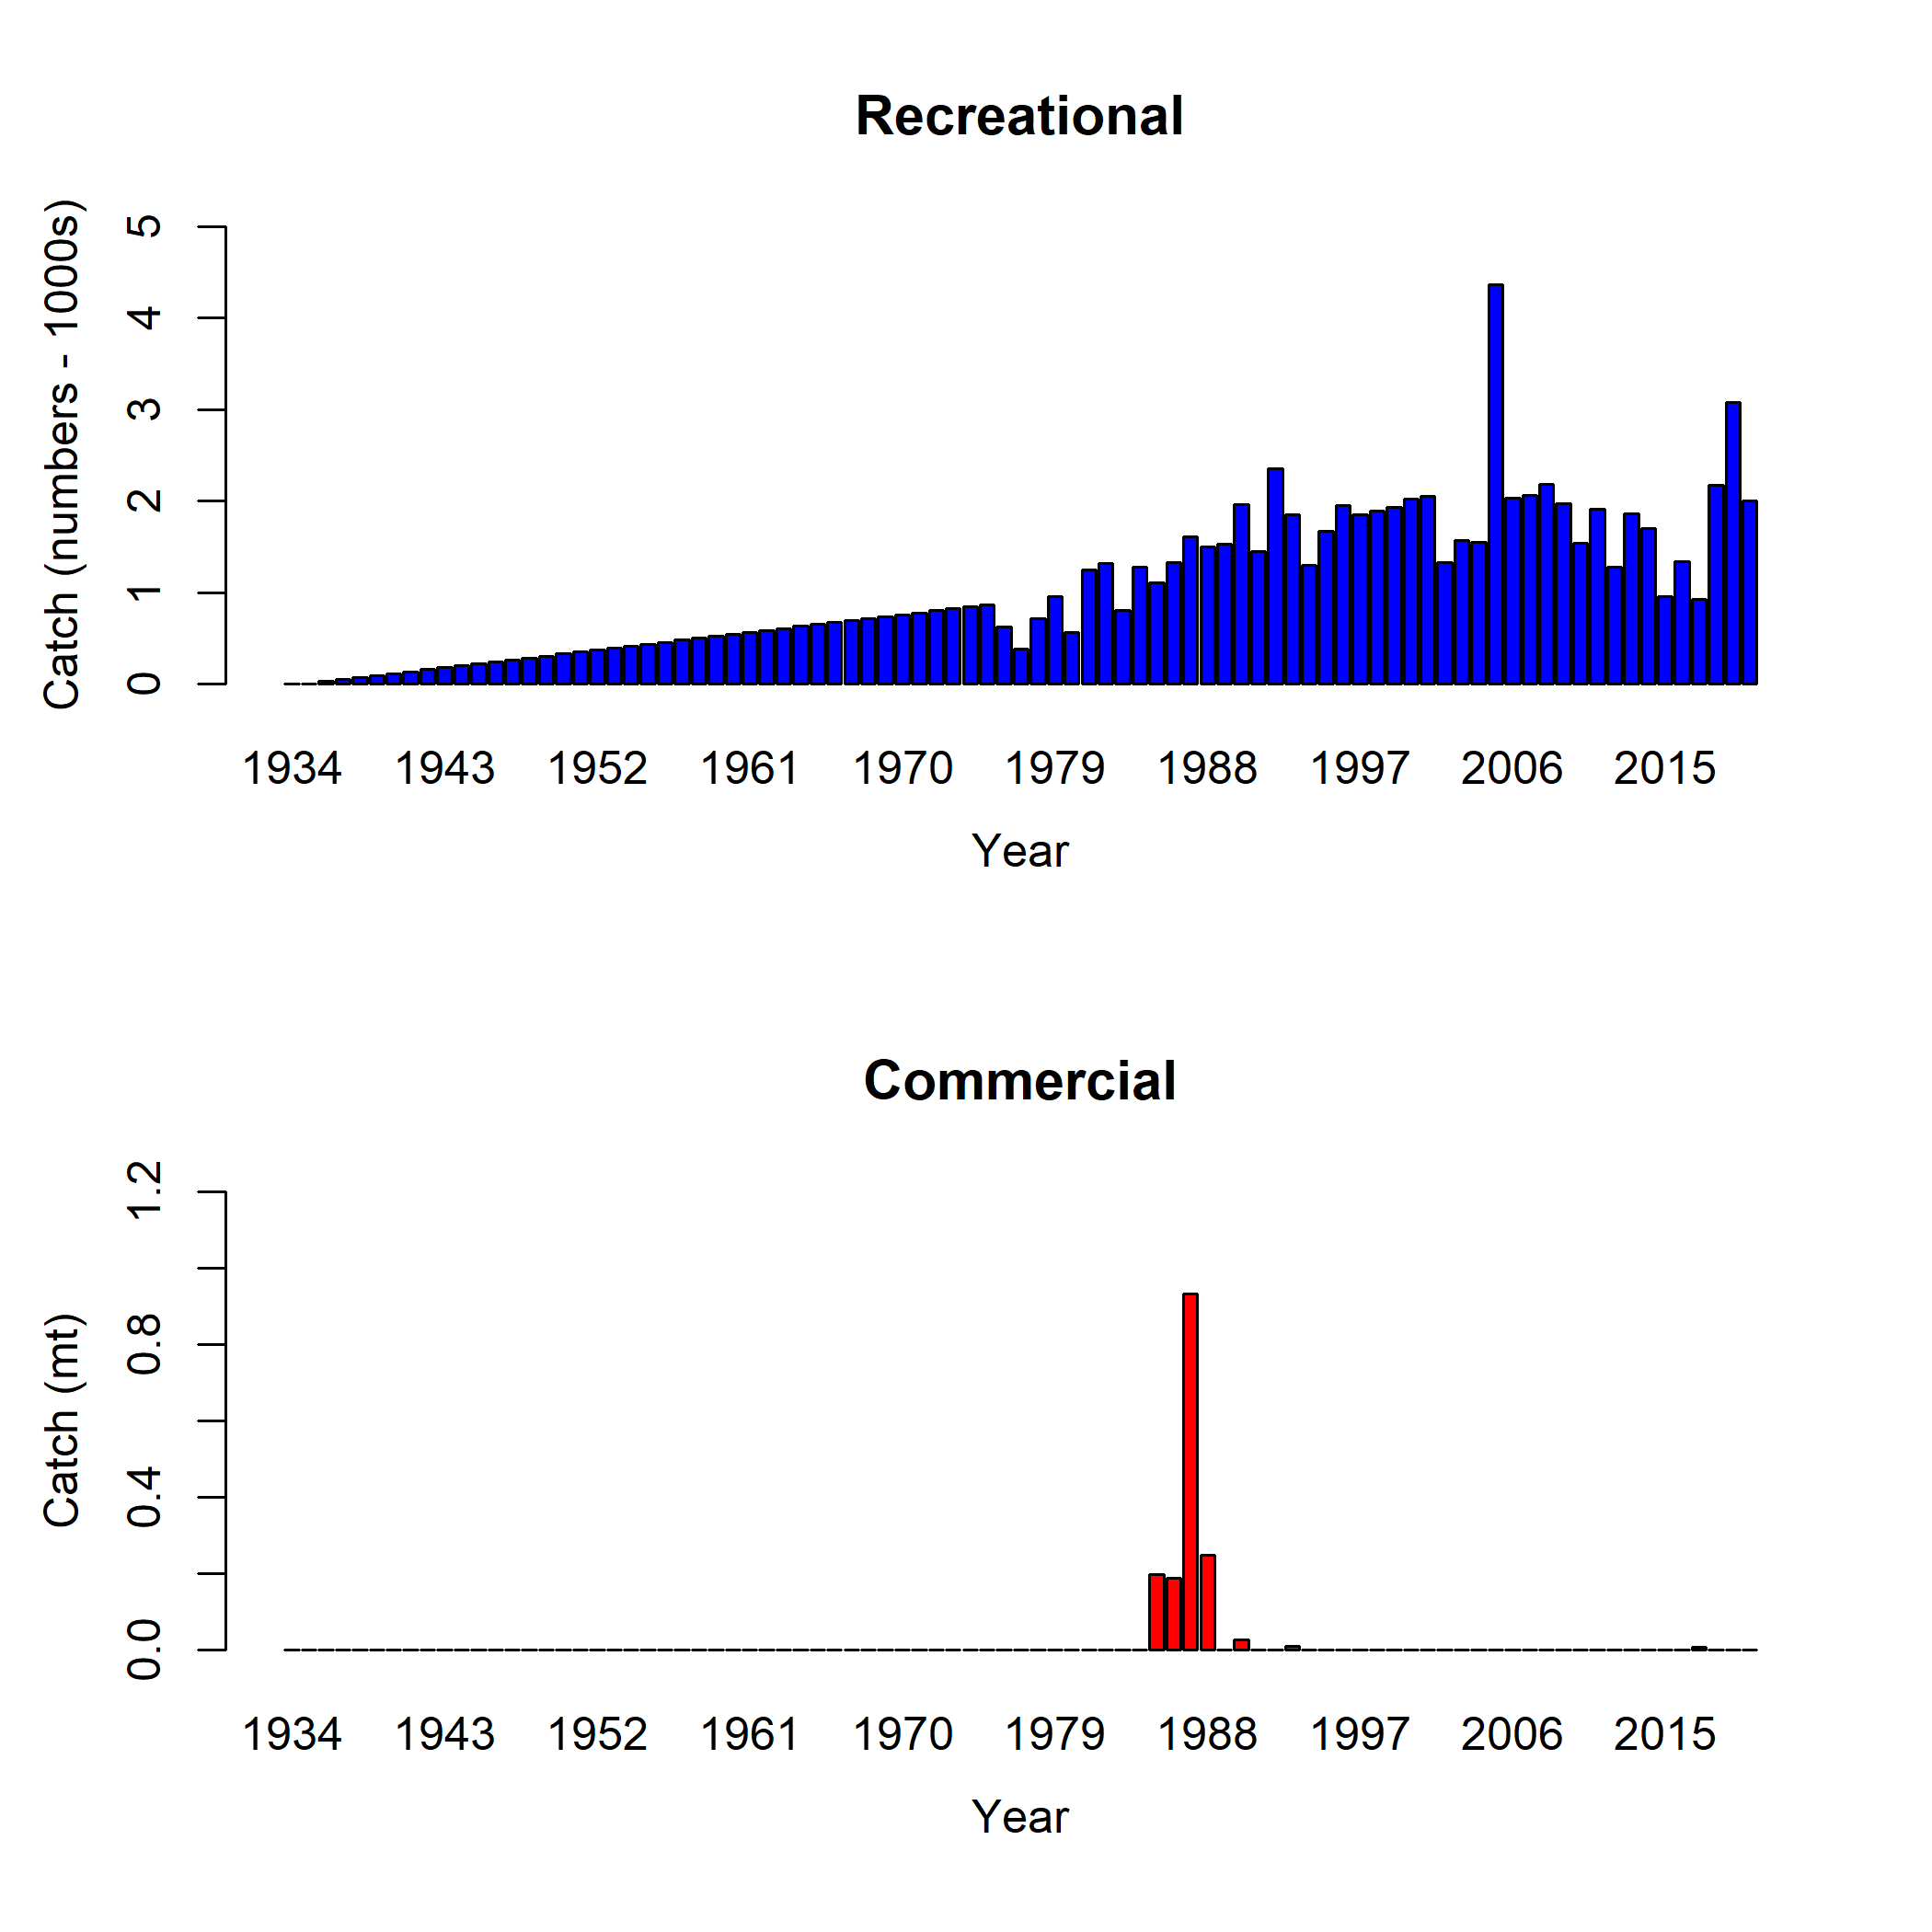
\includegraphics[width=1\textwidth,height=1\textheight]{figs/catches_wa.png}
\caption{Catches by year for the recreational and commercial fleets in the model.\label{fig:catch}}
\end{figure}

\tagmcend\tagstructend

\tagstructbegin{tag=Figure,alttext={Summary of data sources used in the base model.}}\tagmcbegin{tag=Figure}

\begin{figure}
\centering
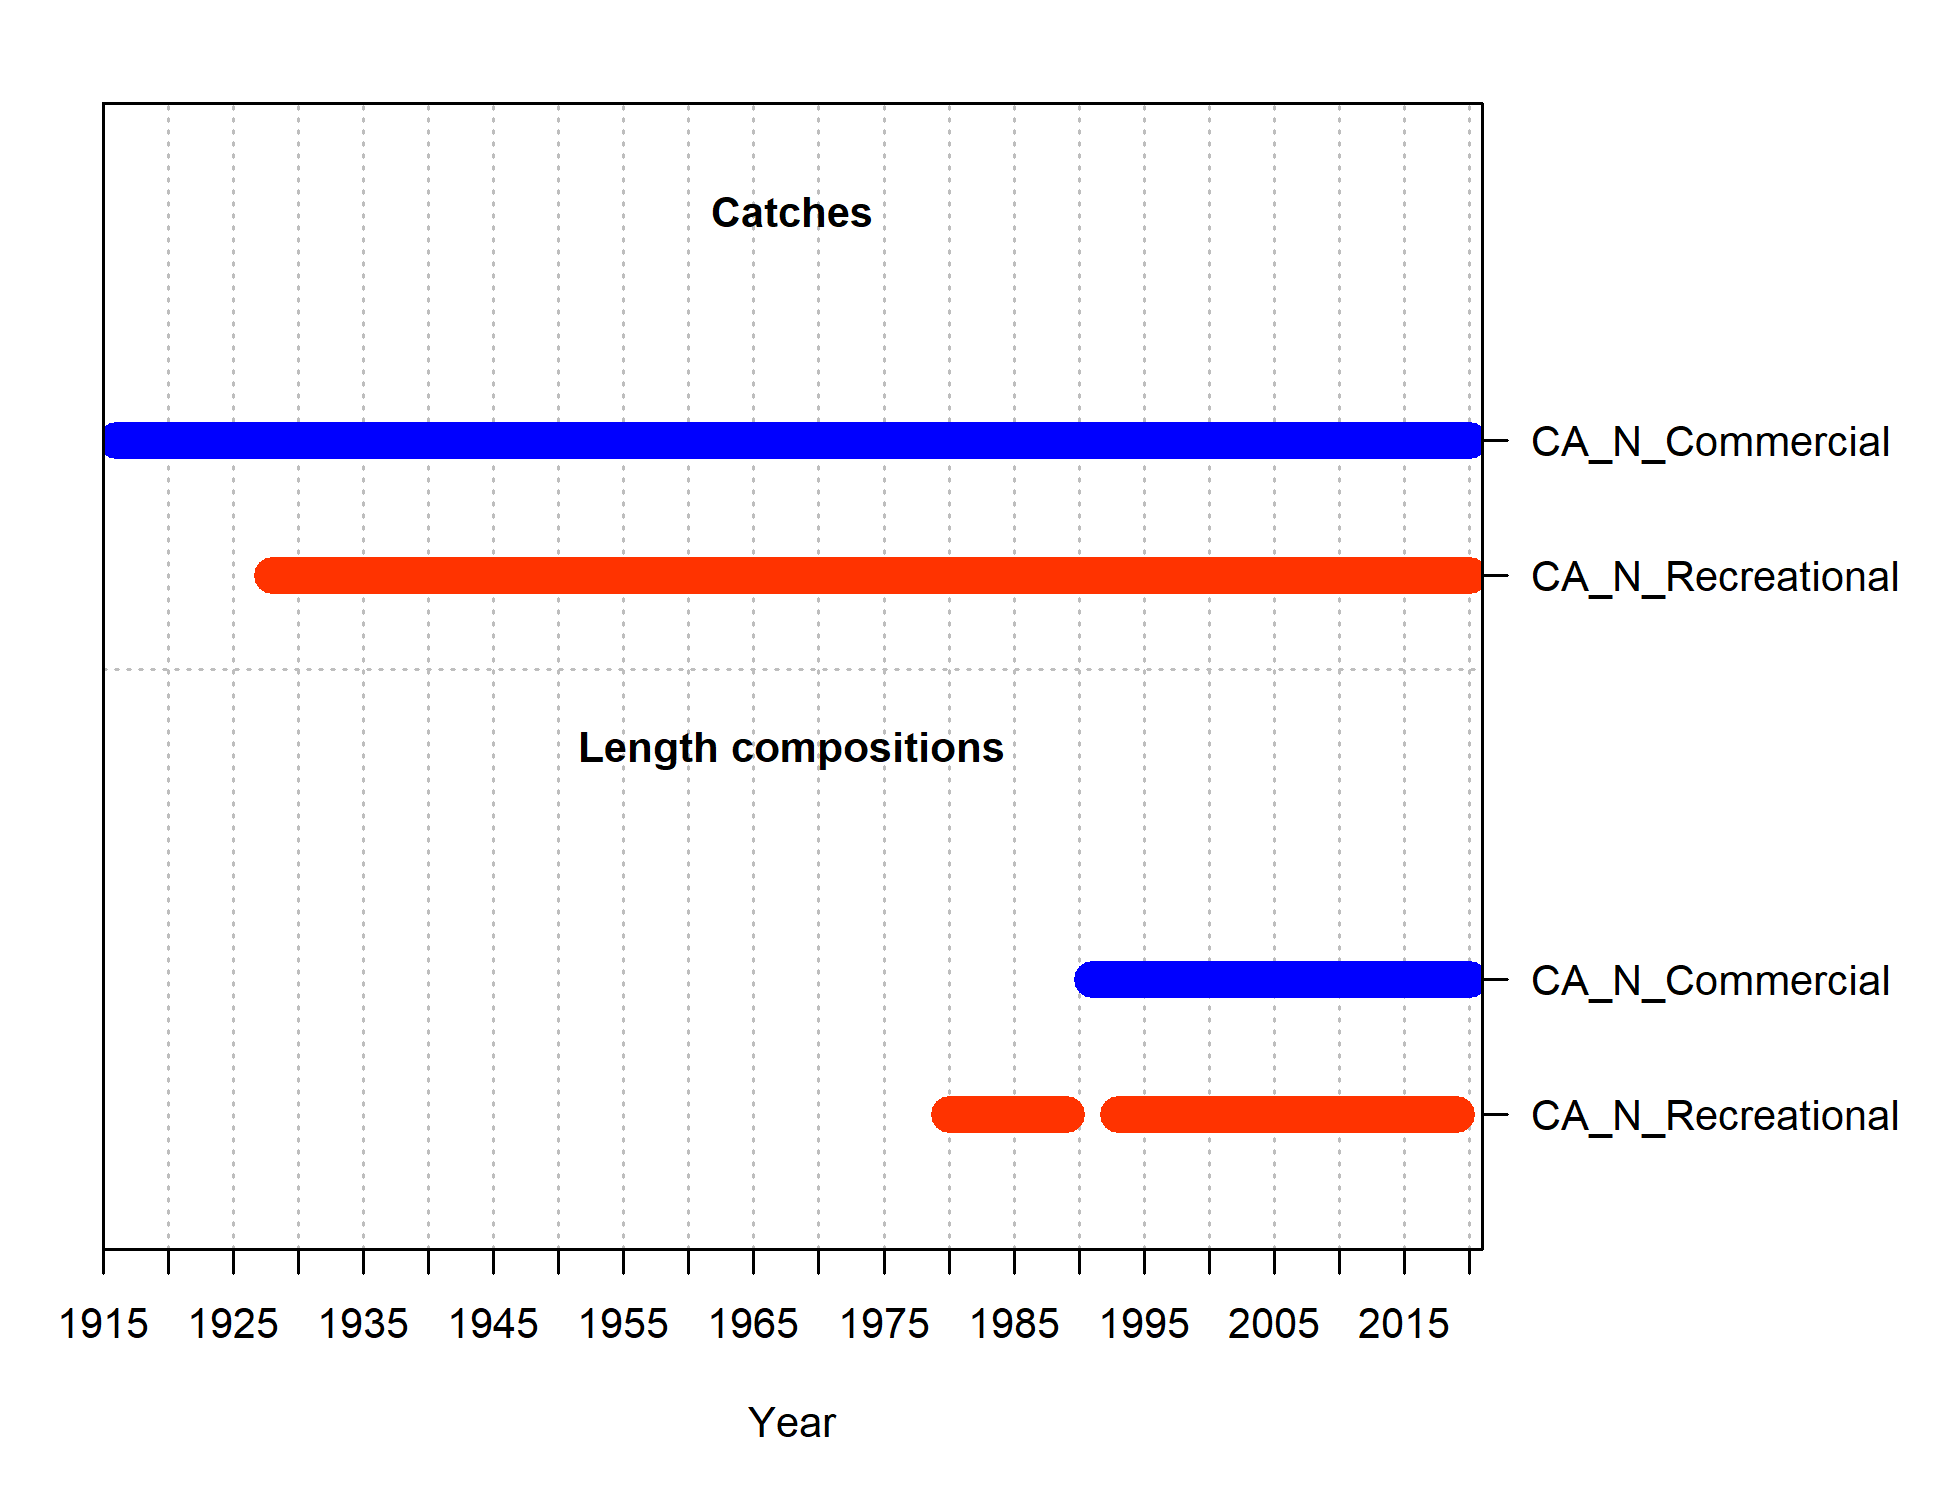
\includegraphics[width=1\textwidth,height=1\textheight]{C:/Assessments/2021/copper_rockfish_2021/models/wa/7.7_base/plots/data_plot.png}
\caption{Summary of data sources used in the base model.\label{fig:data-plot}}
\end{figure}

\tagmcend\tagstructend

\tagstructbegin{tag=Figure,alttext={Length composition data from the recreational fleet.}}\tagmcbegin{tag=Figure}

\begin{figure}
\centering
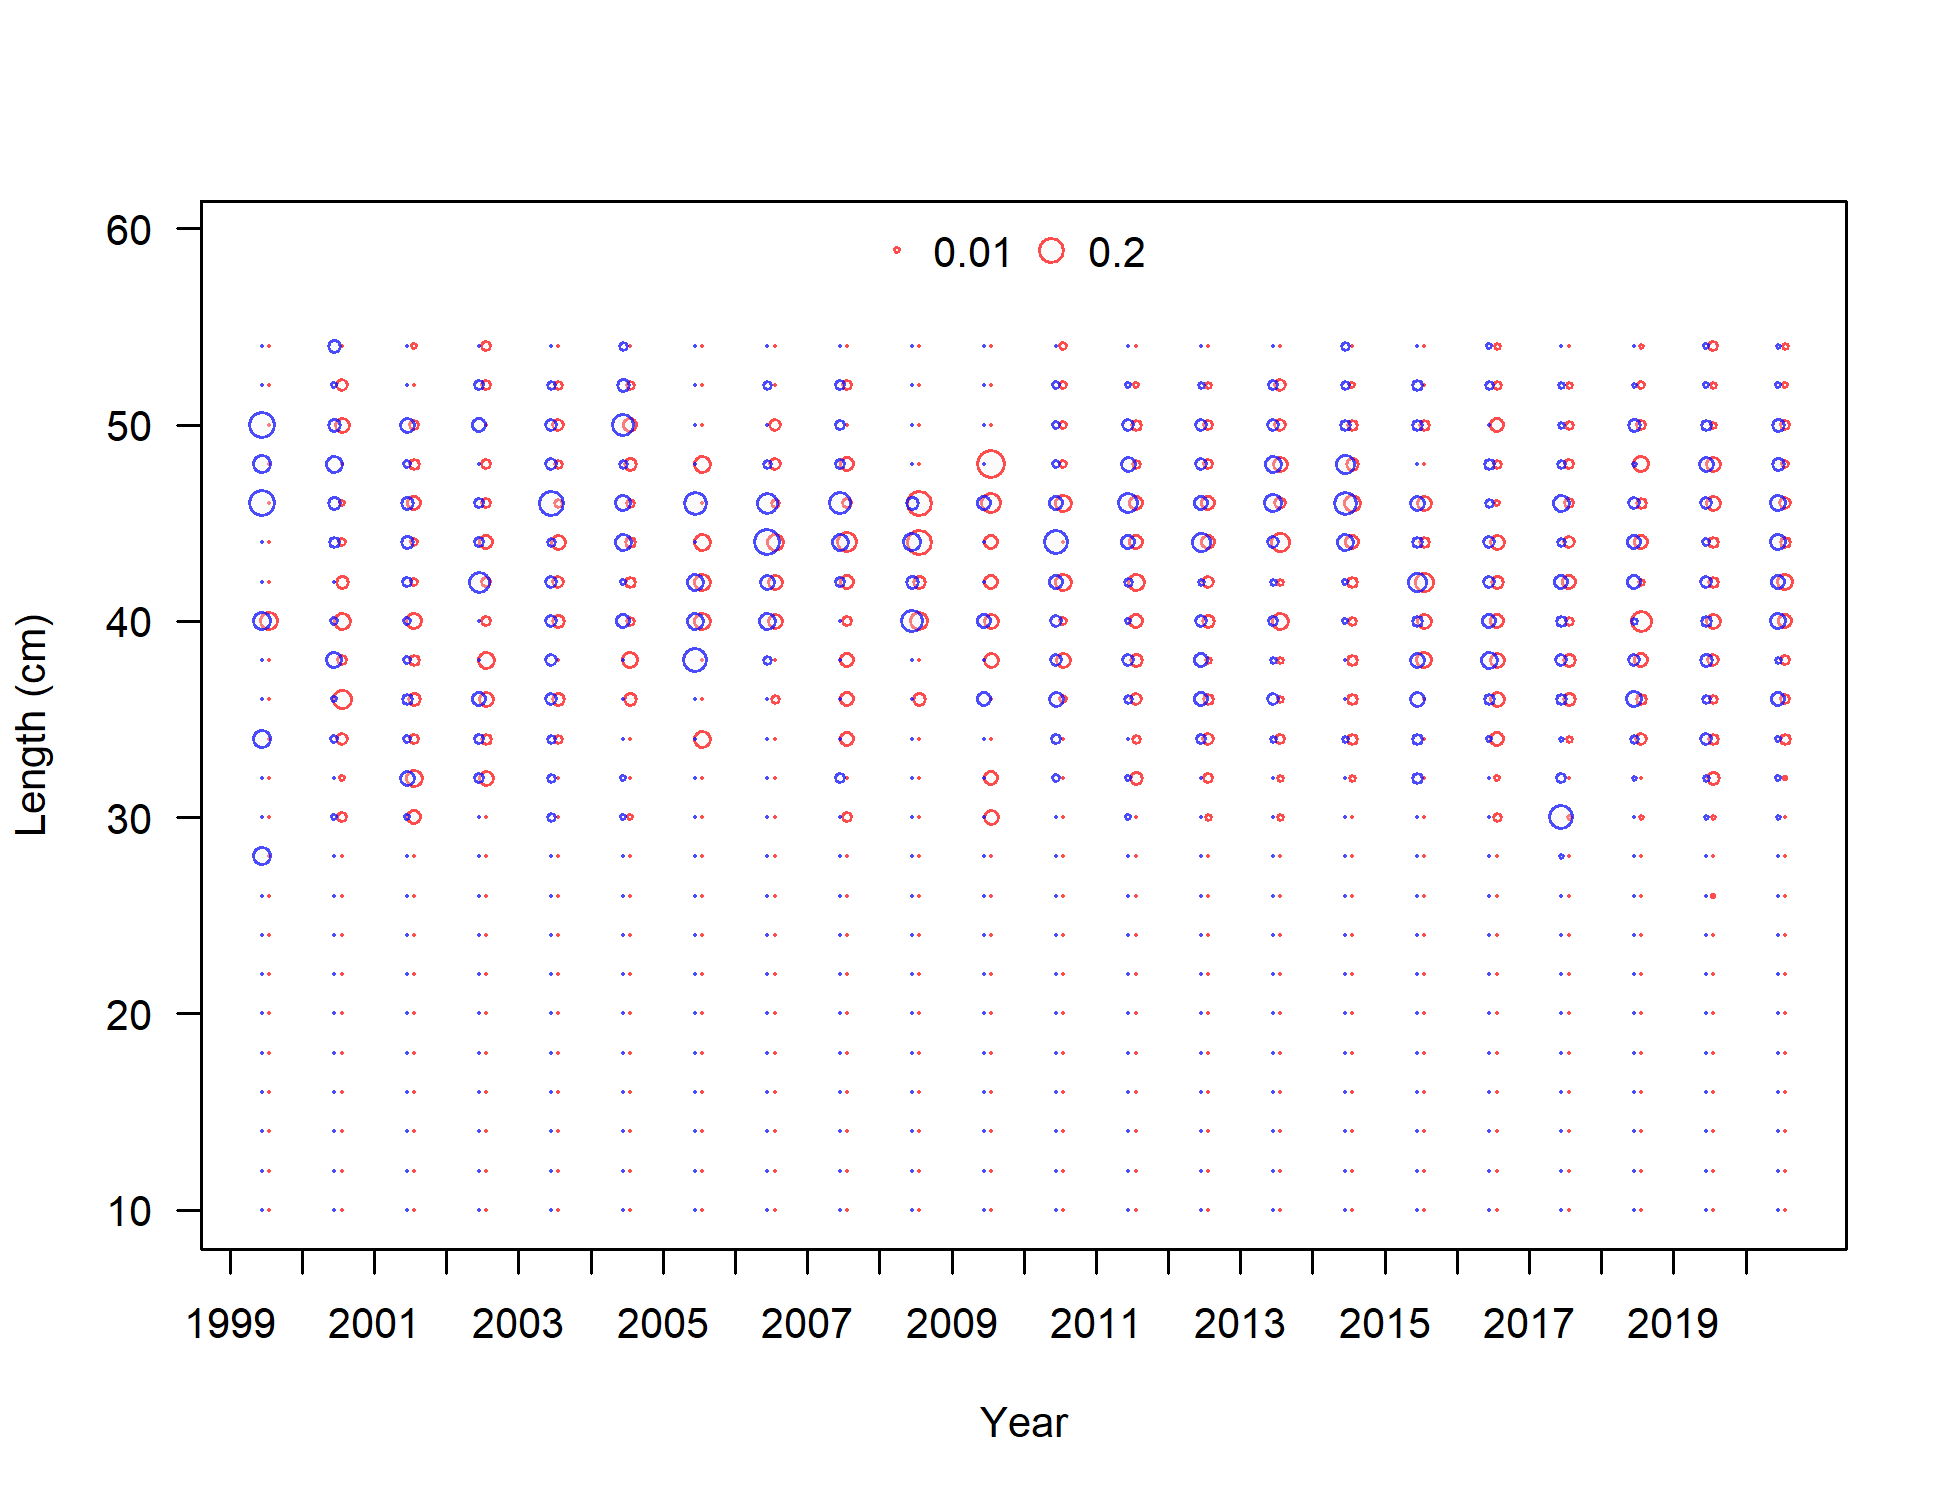
\includegraphics[width=1\textwidth,height=1\textheight]{C:/Assessments/2021/copper_rockfish_2021/models/wa/7.7_base/plots/comp_lendat_bubflt1mkt0_page2.png}
\caption{Length composition data from the recreational fleet.\label{fig:wa-len-data}}
\end{figure}

\tagmcend\tagstructend

\tagstructbegin{tag=Figure,alttext={Aggregated length composition data across all years from the recreational fleet.}}\tagmcbegin{tag=Figure}

\begin{figure}
\centering
\includegraphics[width=1\textwidth,height=1\textheight]{C:/Assessments/2021/copper_rockfish_2021/models/wa/7.7_base/plots/comp_lendat__aggregated_across_time.png}
\caption{Aggregated length composition data across all years from the recreational fleet.\label{fig:wa-len-agg}}
\end{figure}

\tagmcend\tagstructend

\tagstructbegin{tag=Figure,alttext={Mean length for recreational fleet with 95 percent confidence intervals.}}\tagmcbegin{tag=Figure}

\begin{figure}
\centering
\includegraphics[width=1\textwidth,height=1\textheight]{C:/Assessments/2021/copper_rockfish_2021/models/wa/7.7_base/plots/comp_lendat_data_weighting_TA1.8_WA_Recreational.png}
\caption{Mean length for recreational fleet with 95 percent confidence intervals.\label{fig:mean-len-data}}
\end{figure}

\tagmcend\tagstructend

\tagstructbegin{tag=Figure,alttext={Comparison of the length-at-weight data from the NWFSC Hook and Line and the NWFSC WCGBT surveys.}}\tagmcbegin{tag=Figure}

\begin{figure}
\centering
\includegraphics[width=1\textwidth,height=1\textheight]{//nwcfile/FRAM/Assessments/CurrentAssessments/DataModerate_2021/copper_rockfish/data/biology/plots/doc_Length_Weight_Source.png}
\caption{Comparison of the length-at-weight data from the NWFSC Hook and Line and the NWFSC WCGBT surveys.\label{fig:len-weight-survey}}
\end{figure}

\tagmcend\tagstructend

\tagstructbegin{tag=Figure,alttext={Weight-at-length by sex used in the model.}}\tagmcbegin{tag=Figure}

\begin{figure}
\centering
\includegraphics[width=1\textwidth,height=1\textheight]{C:/Assessments/2021/copper_rockfish_2021/models/wa/7.7_base/plots/bio5_weightatsize.png}
\caption{Weight-at-length by sex used in the model.\label{fig:len-weight}}
\end{figure}

\tagmcend\tagstructend

\tagstructbegin{tag=Figure,alttext={Observed sex specific length-at-age by data source with the estimate length-at-age curve.}}\tagmcbegin{tag=Figure}

\begin{figure}
\centering
\includegraphics[width=1\textwidth,height=1\textheight]{//nwcfile/FRAM/Assessments/CurrentAssessments/DataModerate_2021/copper_rockfish/data/biology/plots/doc_north_Age_by_Sex_Source.png}
\caption{Observed sex specific length-at-age by data source with the estimate length-at-age curve.\label{fig:len-age-data}}
\end{figure}

\tagmcend\tagstructend

\tagstructbegin{tag=Figure,alttext={Length at age in the beginning of the year in the ending year of the model.}}\tagmcbegin{tag=Figure}

\begin{figure}
\centering
\includegraphics[width=1\textwidth,height=1\textheight]{C:/Assessments/2021/copper_rockfish_2021/models/wa/7.7_base/plots/bio1_sizeatage.png}
\caption{Length at age in the beginning of the year in the ending year of the model.\label{fig:len-age-ss}}
\end{figure}

\tagmcend\tagstructend

\clearpage

\tagstructbegin{tag=Figure,alttext={Maturity as a function of  length.}}\tagmcbegin{tag=Figure}

\begin{figure}
\centering
\includegraphics[width=1\textwidth,height=1\textheight]{C:/Assessments/2021/copper_rockfish_2021/models/wa/7.7_base/plots/bio6_maturity.png}
\caption{Maturity as a function of length.\label{fig:maturity}}
\end{figure}

\tagmcend\tagstructend

\clearpage

\tagstructbegin{tag=Figure,alttext={Fecundity as a function of length.}}\tagmcbegin{tag=Figure}

\begin{figure}
\centering
\includegraphics[width=1\textwidth,height=1\textheight]{C:/Assessments/2021/copper_rockfish_2021/models/wa/7.7_base/plots/bio9_fecundity_len.png}
\caption{Fecundity as a function of length.\label{fig:fecundity}}
\end{figure}

\tagmcend\tagstructend

\clearpage

\tagstructbegin{tag=Figure,alttext={Fraction female by length across all available data sources.}}\tagmcbegin{tag=Figure}

\begin{figure}
\centering
\includegraphics[width=1\textwidth,height=1\textheight]{//nwcfile/FRAM/Assessments/CurrentAssessments/DataModerate_2021/copper_rockfish/data/biology/plots/Length_fraction_female.png}
\caption{Fraction female by length across all available data sources.\label{fig:len-sex-ratio}}
\end{figure}

\tagmcend\tagstructend

\tagstructbegin{tag=Figure,alttext={Fraction female by age across all available data sources.}}\tagmcbegin{tag=Figure}

\begin{figure}
\centering
\includegraphics[width=1\textwidth,height=1\textheight]{//nwcfile/FRAM/Assessments/CurrentAssessments/DataModerate_2021/copper_rockfish/data/biology/plots/Age_fraction_female.png}
\caption{Fraction female by age across all available data sources.\label{fig:age-sex-ratio}}
\end{figure}

\tagmcend\tagstructend

\tagstructbegin{tag=Figure,alttext={Selectivity at length by fleet.}}\tagmcbegin{tag=Figure}

\begin{figure}
\centering
\includegraphics[width=1\textwidth,height=1\textheight]{C:/Assessments/2021/copper_rockfish_2021/models/wa/7.7_base/plots/sel01_multiple_fleets_length1.png}
\caption{Selectivity at length by fleet.\label{fig:selex}}
\end{figure}

\tagmcend\tagstructend

\tagstructbegin{tag=Figure,alttext={Pearson residuals for recreational fleet. Closed bubble are positive residuals (observed > expected) and open bubbles are negative residuals (observed < expected).}}\tagmcbegin{tag=Figure}

\begin{figure}
\centering
\includegraphics[width=1\textwidth,height=1\textheight]{C:/Assessments/2021/copper_rockfish_2021/models/wa/7.7_base/plots/comp_lenfit_residsflt1mkt0_page2.png}
\caption{Pearson residuals for recreational fleet. Closed bubble are positive residuals (observed \textgreater{} expected) and open bubbles are negative residuals (observed \textless{} expected).\label{fig:rec-pearson}}
\end{figure}

\tagmcend\tagstructend

\tagstructbegin{tag=Figure,alttext={Mean length for recreational with 95 percent confidence intervals based on current samples sizes.}}\tagmcbegin{tag=Figure}

\begin{figure}
\centering
\includegraphics[width=1\textwidth,height=1\textheight]{C:/Assessments/2021/copper_rockfish_2021/models/wa/7.7_base/plots/comp_lenfit_data_weighting_TA1.8_WA_Recreational.png}
\caption{Mean length for recreational with 95 percent confidence intervals based on current samples sizes.\label{fig:rec-mean-len-fit}}
\end{figure}

\tagmcend\tagstructend

\tagstructbegin{tag=Figure,alttext={Aggregated length comps across all years.}}\tagmcbegin{tag=Figure}

\begin{figure}
\centering
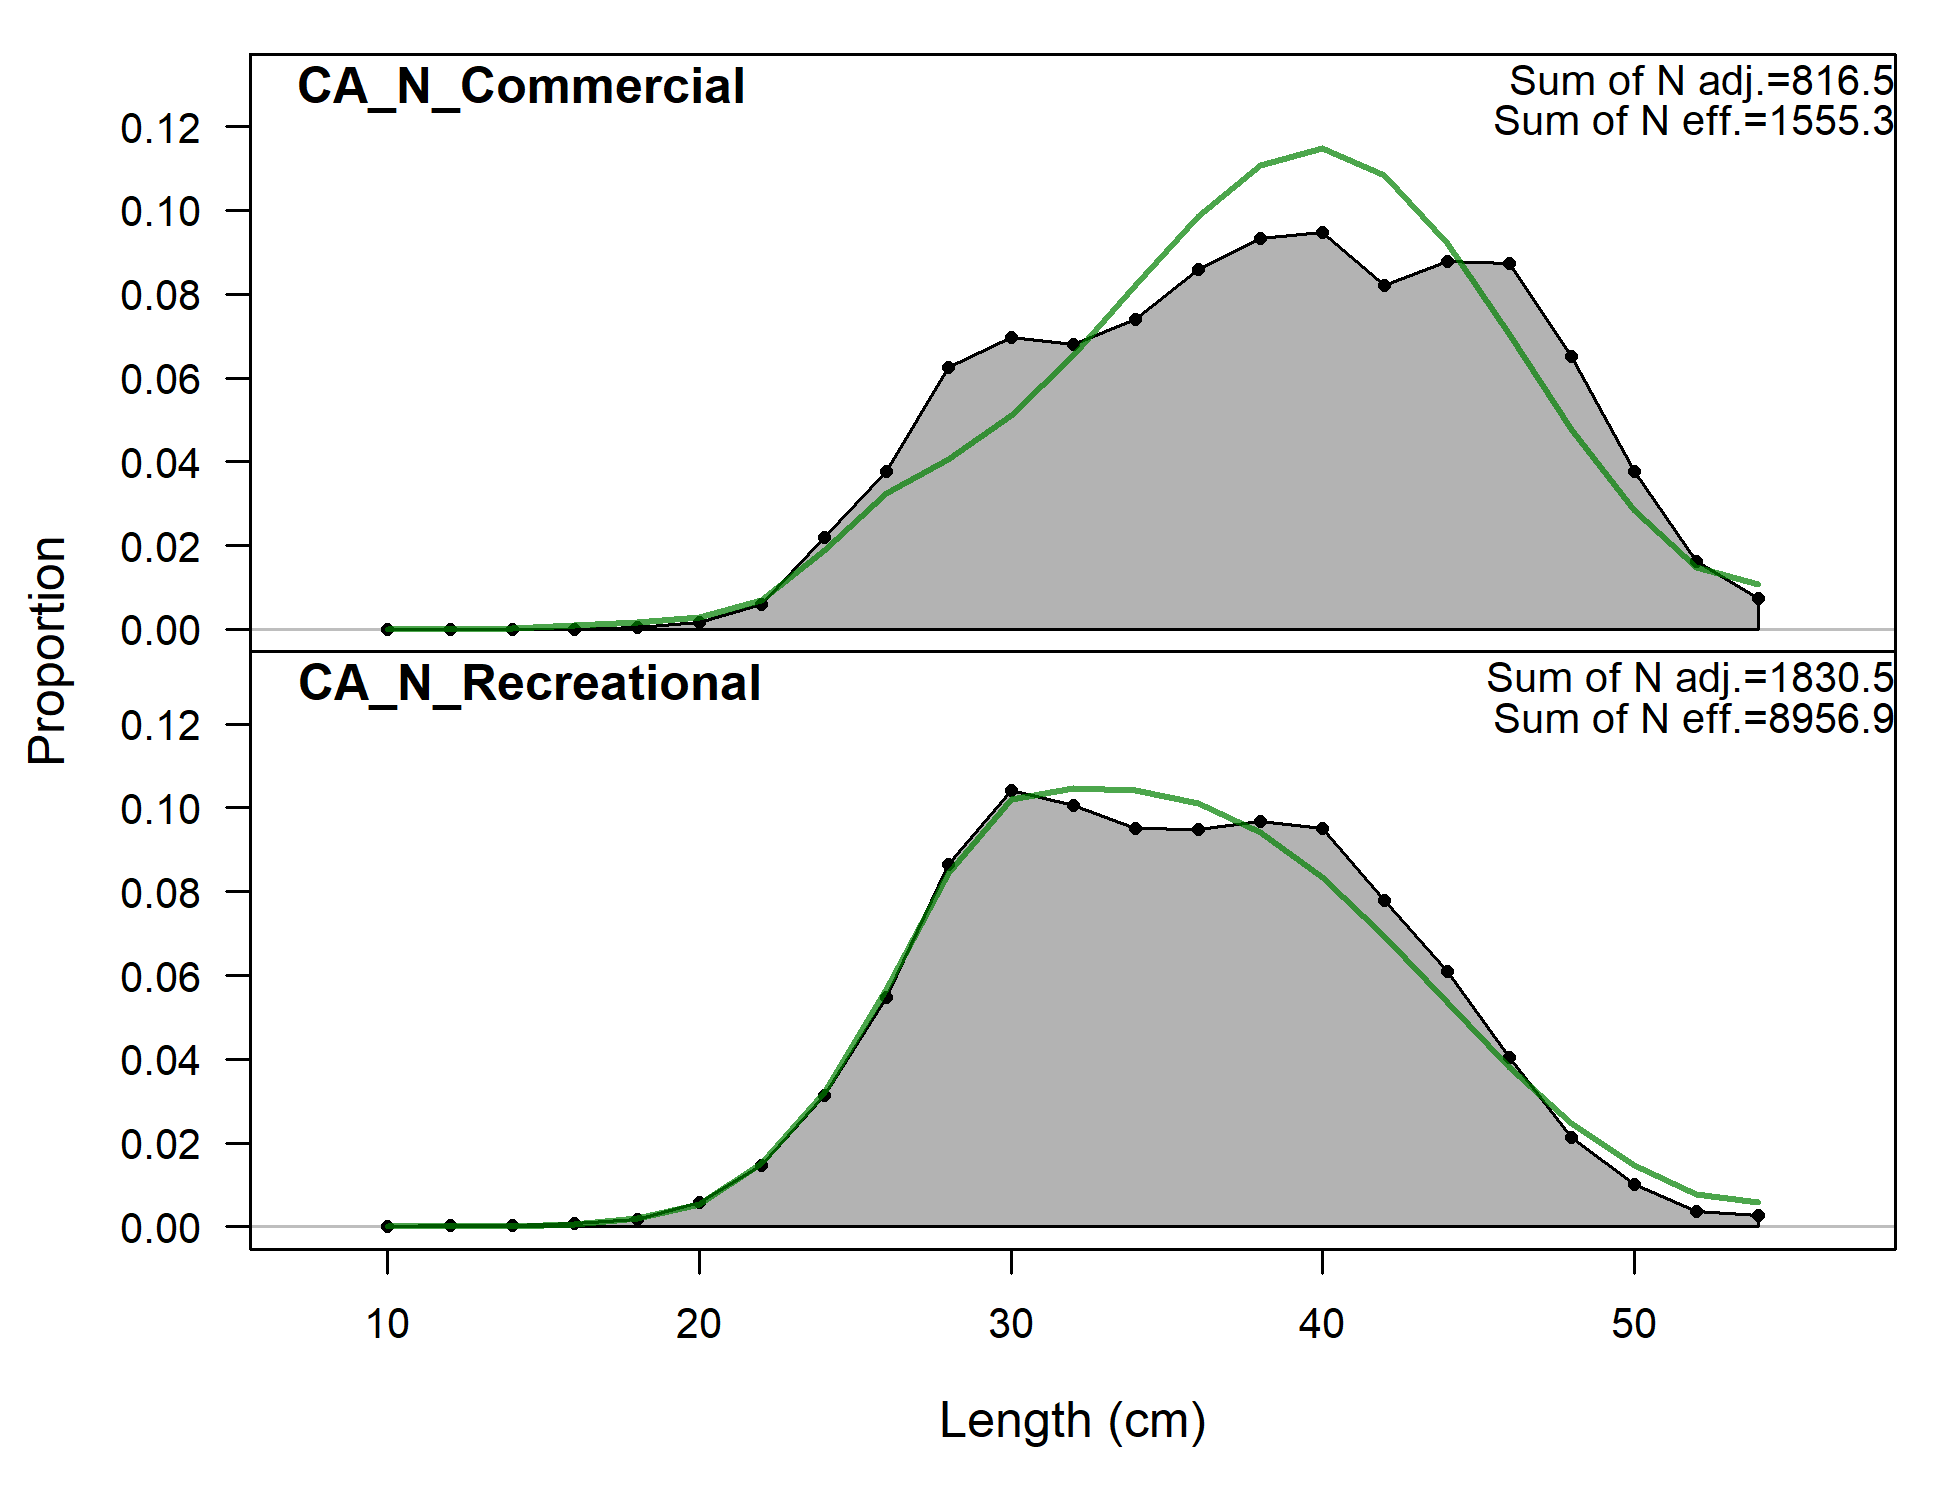
\includegraphics[width=1\textwidth,height=1\textheight]{C:/Assessments/2021/copper_rockfish_2021/models/wa/7.7_base/plots/comp_lenfit__aggregated_across_time.png}
\caption{Aggregated length comps across all years.\label{fig:agg-len-fit}}
\end{figure}

\tagmcend\tagstructend

\tagstructbegin{tag=Figure,alttext={Estimated time series of spawning output.}}\tagmcbegin{tag=Figure}

\begin{figure}
\centering
\includegraphics[width=1\textwidth,height=1\textheight]{C:/Assessments/2021/copper_rockfish_2021/models/wa/7.7_base/plots/ts7_Spawning_output_with_95_asymptotic_intervals_intervals.png}
\caption{Estimated time series of spawning output.\label{fig:ssb}}
\end{figure}

\tagmcend\tagstructend

\tagstructbegin{tag=Figure,alttext={Estimated time series of total biomass.}}\tagmcbegin{tag=Figure}

\begin{figure}
\centering
\includegraphics[width=1\textwidth,height=1\textheight]{C:/Assessments/2021/copper_rockfish_2021/models/wa/7.7_base/plots/ts1_Total_biomass_(mt).png}
\caption{Estimated time series of total biomass.\label{fig:tot-bio}}
\end{figure}

\tagmcend\tagstructend

\tagstructbegin{tag=Figure,alttext={Estimated time series of fraction of unfished spawning output.}}\tagmcbegin{tag=Figure}

\begin{figure}
\centering
\includegraphics[width=1\textwidth,height=1\textheight]{C:/Assessments/2021/copper_rockfish_2021/models/wa/7.7_base/plots/ts9_Fraction_of_unfished_with_95_asymptotic_intervals_intervals.png}
\caption{Estimated time series of fraction of unfished spawning output.\label{fig:depl}}
\end{figure}

\tagmcend\tagstructend

\tagstructbegin{tag=Figure,alttext={Stock-recruit curve. Point colors indicate year, with warmer colors indicating earlier years and cooler colors in showing later years.}}\tagmcbegin{tag=Figure}

\begin{figure}
\centering
\includegraphics[width=1\textwidth,height=1\textheight]{C:/Assessments/2021/copper_rockfish_2021/models/wa/7.7_base/plots/SR_curve.png}
\caption{Stock-recruit curve. Point colors indicate year, with warmer colors indicating earlier years and cooler colors in showing later years.\label{fig:bh-curve}}
\end{figure}

\tagmcend\tagstructend

\tagstructbegin{tag=Figure,alttext={Estimated time series of age-0 recruits (1000s).}}\tagmcbegin{tag=Figure}

\begin{figure}
\centering
\includegraphics[width=1\textwidth,height=1\textheight]{C:/Assessments/2021/copper_rockfish_2021/models/wa/7.7_base/plots/ts11_Age-0_recruits_(1000s)_with_95_asymptotic_intervals.png}
\caption{Estimated time series of age-0 recruits (1000s).\label{fig:recruits}}
\end{figure}

\tagmcend\tagstructend

\tagstructbegin{tag=Figure,alttext={Change in estimated spawning output by sensitivity.}}\tagmcbegin{tag=Figure}

\begin{figure}
\centering
\includegraphics[width=1\textwidth,height=1\textheight]{C:/Assessments/2021/copper_rockfish_2021/models/wa/_sensitivities/_plots/7.7_base_compare2_spawnbio_uncertainty.png}
\caption{Change in estimated spawning output by sensitivity.\label{fig:sens-ssb}}
\end{figure}

\tagmcend\tagstructend

\tagstructbegin{tag=Figure,alttext={Change in estimated fraction unfished by sensitivity.}}\tagmcbegin{tag=Figure}

\begin{figure}
\centering
\includegraphics[width=1\textwidth,height=1\textheight]{C:/Assessments/2021/copper_rockfish_2021/models/wa/_sensitivities/_plots/7.7_base_compare4_Bratio_uncertainty.png}
\caption{Change in estimated fraction unfished by sensitivity.\label{fig:sens-depl}}
\end{figure}

\tagmcend\tagstructend

\tagstructbegin{tag=Figure,alttext={Change in estimated annual recruitment deviations by sensitivity.}}\tagmcbegin{tag=Figure}

\begin{figure}
\centering
\includegraphics[width=1\textwidth,height=1\textheight]{C:/Assessments/2021/copper_rockfish_2021/models/wa/_sensitivities/_plots/7.7_base_compare12_recdevs_uncertainty.png}
\caption{Change in estimated annual recruitment deviations by sensitivity.\label{fig:sens-recr}}
\end{figure}

\tagmcend\tagstructend

\tagstructbegin{tag=Figure,alttext={Change in the negative log-likelihood across a range of log(R0) values.}}\tagmcbegin{tag=Figure}

\begin{figure}
\centering
\includegraphics[width=1\textwidth,height=1\textheight]{C:/Assessments/2021/copper_rockfish_2021/models/wa/7.7_base_profile_SR_LN(R0)/piner_panel_SR_LN(R0).png}
\caption{Change in the negative log-likelihood across a range of log(R0) values.\label{fig:r0-profile}}
\end{figure}

\tagmcend\tagstructend

\tagstructbegin{tag=Figure,alttext={Change in the estimate of spawning output across a range of log(R0) values.}}\tagmcbegin{tag=Figure}

\begin{figure}
\centering
\includegraphics[width=1\textwidth,height=1\textheight]{C:/Assessments/2021/copper_rockfish_2021/models/wa/7.7_base_profile_SR_LN(R0)/SR_LN(R0)_trajectories_compare1_spawnbio.png}
\caption{Change in the estimate of spawning output across a range of log(R0) values.\label{fig:r0-ssb}}
\end{figure}

\tagmcend\tagstructend

\tagstructbegin{tag=Figure,alttext={Change in the estimate of fraction unfished across a range of log(R0) values.}}\tagmcbegin{tag=Figure}

\begin{figure}
\centering
\includegraphics[width=1\textwidth,height=1\textheight]{C:/Assessments/2021/copper_rockfish_2021/models/wa/7.7_base_profile_SR_LN(R0)/SR_LN(R0)_trajectories_compare3_Bratio.png}
\caption{Change in the estimate of fraction unfished across a range of log(R0) values.\label{fig:r0-depl}}
\end{figure}

\tagmcend\tagstructend

\tagstructbegin{tag=Figure,alttext={Change in the negative log-likelihood across a range of steepness values.}}\tagmcbegin{tag=Figure}

\begin{figure}
\centering
\includegraphics[width=1\textwidth,height=1\textheight]{C:/Assessments/2021/copper_rockfish_2021/models/wa/7.7_base_profile_SR_BH_steep/piner_panel_SR_BH_steep.png}
\caption{Change in the negative log-likelihood across a range of steepness values.\label{fig:h-profile}}
\end{figure}

\tagmcend\tagstructend

\tagstructbegin{tag=Figure,alttext={Change in the estimate of spawning output across a range of steepness values.}}\tagmcbegin{tag=Figure}

\begin{figure}
\centering
\includegraphics[width=1\textwidth,height=1\textheight]{C:/Assessments/2021/copper_rockfish_2021/models/wa/7.7_base_profile_SR_BH_steep/SR_BH_steep_trajectories_compare1_spawnbio.png}
\caption{Change in the estimate of spawning output across a range of steepness values.\label{fig:h-ssb}}
\end{figure}

\tagmcend\tagstructend

\tagstructbegin{tag=Figure,alttext={Change in the estimate of fraction unfished across a range of steepness values.}}\tagmcbegin{tag=Figure}

\begin{figure}
\centering
\includegraphics[width=1\textwidth,height=1\textheight]{C:/Assessments/2021/copper_rockfish_2021/models/wa/7.7_base_profile_SR_BH_steep/SR_BH_steep_trajectories_compare3_Bratio.png}
\caption{Change in the estimate of fraction unfished across a range of steepness values.\label{fig:h-depl}}
\end{figure}

\tagmcend\tagstructend

\tagstructbegin{tag=Figure,alttext={Change in the negative log-likelihood across a range of female natural mortality values.}}\tagmcbegin{tag=Figure}

\begin{figure}
\centering
\includegraphics[width=1\textwidth,height=1\textheight]{C:/Assessments/2021/copper_rockfish_2021/models/wa/7.7_base_profile_NatM_p_1_Fem_GP_1/piner_panel_NatM_p_1_Fem_GP_1.png}
\caption{Change in the negative log-likelihood across a range of female natural mortality values.\label{fig:m-profile}}
\end{figure}

\tagmcend\tagstructend

\tagstructbegin{tag=Figure,alttext={Change in the estimate of spawning output across a range of female natural mortality values.}}\tagmcbegin{tag=Figure}

\begin{figure}
\centering
\includegraphics[width=1\textwidth,height=1\textheight]{C:/Assessments/2021/copper_rockfish_2021/models/wa/7.7_base_profile_NatM_p_1_Fem_GP_1/NatM_p_1_Fem_GP_1_trajectories_compare1_spawnbio.png}
\caption{Change in the estimate of spawning output across a range of female natural mortality values.\label{fig:m-ssb}}
\end{figure}

\tagmcend\tagstructend

\tagstructbegin{tag=Figure,alttext={Change in the estimate of fraction unfished across a range of female natural values.}}\tagmcbegin{tag=Figure}

\begin{figure}
\centering
\includegraphics[width=1\textwidth,height=1\textheight]{C:/Assessments/2021/copper_rockfish_2021/models/wa/7.7_base_profile_NatM_p_1_Fem_GP_1/NatM_p_1_Fem_GP_1_trajectories_compare3_Bratio.png}
\caption{Change in the estimate of fraction unfished across a range of female natural values.\label{fig:m-depl}}
\end{figure}

\tagmcend\tagstructend

\tagstructbegin{tag=Figure,alttext={Change in the negative log-likelihood across a range of female maximum length values.}}\tagmcbegin{tag=Figure}

\begin{figure}
\centering
\includegraphics[width=1\textwidth,height=1\textheight]{C:/Assessments/2021/copper_rockfish_2021/models/wa/7.7_base_profile_L_at_Amax_Fem_GP_1/piner_panel_L_at_Amax_Fem_GP_1.png}
\caption{Change in the negative log-likelihood across a range of female maximum length values.\label{fig:linf-profile}}
\end{figure}

\tagmcend\tagstructend

\tagstructbegin{tag=Figure,alttext={Change in the estimate of spawning output across a range of female maximum length values.}}\tagmcbegin{tag=Figure}

\begin{figure}
\centering
\includegraphics[width=1\textwidth,height=1\textheight]{C:/Assessments/2021/copper_rockfish_2021/models/wa/7.7_base_profile_L_at_Amax_Fem_GP_1/L_at_Amax_Fem_GP_1_trajectories_compare1_spawnbio.png}
\caption{Change in the estimate of spawning output across a range of female maximum length values.\label{fig:linf-ssb}}
\end{figure}

\tagmcend\tagstructend

\tagstructbegin{tag=Figure,alttext={Change in the estimate of fraction unfished across a range of female maximum length values.}}\tagmcbegin{tag=Figure}

\begin{figure}
\centering
\includegraphics[width=1\textwidth,height=1\textheight]{C:/Assessments/2021/copper_rockfish_2021/models/wa/7.7_base_profile_L_at_Amax_Fem_GP_1/L_at_Amax_Fem_GP_1_trajectories_compare3_Bratio.png}
\caption{Change in the estimate of fraction unfished across a range of female maximum length values.\label{fig:linf-depl}}
\end{figure}

\tagmcend\tagstructend

\tagstructbegin{tag=Figure,alttext={Change in the negative log-likelihood across a range of female k values.}}\tagmcbegin{tag=Figure}

\begin{figure}
\centering
\includegraphics[width=1\textwidth,height=1\textheight]{C:/Assessments/2021/copper_rockfish_2021/models/wa/7.7_base_profile_VonBert_K_Fem_GP_1/piner_panel_VonBert_K_Fem_GP_1.png}
\caption{Change in the negative log-likelihood across a range of female k values.\label{fig:k-profile}}
\end{figure}

\tagmcend\tagstructend

\tagstructbegin{tag=Figure,alttext={Change in the estimate of spawning output across a range of female k values.}}\tagmcbegin{tag=Figure}

\begin{figure}
\centering
\includegraphics[width=1\textwidth,height=1\textheight]{C:/Assessments/2021/copper_rockfish_2021/models/wa/7.7_base_profile_VonBert_K_Fem_GP_1/VonBert_K_Fem_GP_1_trajectories_compare1_spawnbio.png}
\caption{Change in the estimate of spawning output across a range of female k values.\label{fig:k-ssb}}
\end{figure}

\tagmcend\tagstructend

\tagstructbegin{tag=Figure,alttext={Change in the estimate of fraction unfished across a range of female k values.}}\tagmcbegin{tag=Figure}

\begin{figure}
\centering
\includegraphics[width=1\textwidth,height=1\textheight]{C:/Assessments/2021/copper_rockfish_2021/models/wa/7.7_base_profile_VonBert_K_Fem_GP_1/VonBert_K_Fem_GP_1_trajectories_compare3_Bratio.png}
\caption{Change in the estimate of fraction unfished across a range of female k values.\label{fig:k-depl}}
\end{figure}

\tagmcend\tagstructend

\tagstructbegin{tag=Figure,alttext={Change in the negative log-likelihood across a range of female coefficient of variation for older ages.}}\tagmcbegin{tag=Figure}

\begin{figure}
\centering
\includegraphics[width=1\textwidth,height=1\textheight]{C:/Assessments/2021/copper_rockfish_2021/models/wa/7.7_base_profile_CV_old_Fem_GP_1/piner_panel_CV_old_Fem_GP_1.png}
\caption{Change in the negative log-likelihood across a range of female coefficient of variation for older ages.\label{fig:cv-profile}}
\end{figure}

\tagmcend\tagstructend

\tagstructbegin{tag=Figure,alttext={Change in the estimate of spawning output across a range of female coefficient of variation for older ages.}}\tagmcbegin{tag=Figure}

\begin{figure}
\centering
\includegraphics[width=1\textwidth,height=1\textheight]{C:/Assessments/2021/copper_rockfish_2021/models/wa/7.7_base_profile_CV_old_Fem_GP_1/CV_old_Fem_GP_1_trajectories_compare1_spawnbio.png}
\caption{Change in the estimate of spawning output across a range of female coefficient of variation for older ages.\label{fig:cv-ssb}}
\end{figure}

\tagmcend\tagstructend

\tagstructbegin{tag=Figure,alttext={Change in the estimate of fraction unfished across a range of female coefficient of variation for older ages.}}\tagmcbegin{tag=Figure}

\begin{figure}
\centering
\includegraphics[width=1\textwidth,height=1\textheight]{C:/Assessments/2021/copper_rockfish_2021/models/wa/7.7_base_profile_CV_old_Fem_GP_1/CV_old_Fem_GP_1_trajectories_compare3_Bratio.png}
\caption{Change in the estimate of fraction unfished across a range of female coefficient of variation for older ages.\label{fig:cv-depl}}
\end{figure}

\tagmcend\tagstructend

\newpage

\tagstructbegin{tag=Figure,alttext={LB-SPR yearly estimates of selectivity, the ratio of fishing intensity to natural mortality (F/M), and annual spawner-per-recruit (SPR) values.}}\tagmcbegin{tag=Figure}

\begin{figure}
\centering
\includegraphics[width=1\textwidth,height=1\textheight]{C:/Assessments/2021/copper_rockfish_2021/models/lbspr/Copper_WA_LBSPR_newVBGF_plots.png}
\caption{LB-SPR yearly estimates of selectivity, the ratio of fishing intensity to natural mortality (F/M), and annual spawner-per-recruit (SPR) values.\label{fig:lbspr}}
\end{figure}

\tagmcend\tagstructend

\newpage

\tagstructbegin{tag=Figure,alttext={Prior distributions for parameter input for SSS.}}\tagmcbegin{tag=Figure}

\begin{figure}
\centering
\includegraphics[width=1\textwidth,height=1\textheight]{C:/Assessments/2021/copper_rockfish_2021/models/sss/wa/_plots/7.7_base_depl_67_Priors.png}
\caption{Prior distributions for parameter input for SSS.\label{fig:sss-prior-67}}
\end{figure}

\tagmcend\tagstructend

\newpage

\tagstructbegin{tag=Figure,alttext={Derived quantities from SSS run where fraction unfished was assumed to be 60 percent.}}\tagmcbegin{tag=Figure}

\begin{figure}
\centering
\includegraphics[width=1\textwidth,height=1\textheight]{C:/Assessments/2021/copper_rockfish_2021/models/sss/wa/_plots/7.7_base_depl_67_quants.png}
\caption{Derived quantities from SSS run where fraction unfished was assumed to be 60 percent.\label{fig:sss-quant-67}}
\end{figure}

\tagmcend\tagstructend

\newpage

\tagstructbegin{tag=Figure,alttext={Prior distributions for parameter input for SSS.}}\tagmcbegin{tag=Figure}

\begin{figure}
\centering
\includegraphics[width=1\textwidth,height=1\textheight]{C:/Assessments/2021/copper_rockfish_2021/models/sss/wa/_plots/7.7_base_depl_44_Priors.png}
\caption{Prior distributions for parameter input for SSS.\label{fig:sss-prior-44}}
\end{figure}

\tagmcend\tagstructend

\newpage

\tagstructbegin{tag=Figure,alttext={Derived quantities from SSS run where fraction unfished was assumed to be 40 percent.}}\tagmcbegin{tag=Figure}

\begin{figure}
\centering
\includegraphics[width=1\textwidth,height=1\textheight]{C:/Assessments/2021/copper_rockfish_2021/models/sss/wa/_plots/7.7_base_depl_44_quants.png}
\caption{Derived quantities from SSS run where fraction unfished was assumed to be 40 percent.\label{fig:sss-quant-44}}
\end{figure}

\tagmcend\tagstructend

\newpage

\tagstructbegin{tag=Figure,alttext={Change in the estimate of spawning output when the most recent 5 years of data area removed sequentially.}}\tagmcbegin{tag=Figure}

\begin{figure}
\centering
\includegraphics[width=1\textwidth,height=1\textheight]{C:/Assessments/2021/copper_rockfish_2021/models/wa/7.7_base_retro/compare2_spawnbio_uncertainty.png}
\caption{Change in the estimate of spawning output when the most recent 5 years of data area removed sequentially.\label{fig:retro-ssb}}
\end{figure}

\tagmcend\tagstructend

\tagstructbegin{tag=Figure,alttext={Change in the estimate of fraction unfished when the most recent 5 years of data area removed sequentially.}}\tagmcbegin{tag=Figure}

\begin{figure}
\centering
\includegraphics[width=1\textwidth,height=1\textheight]{C:/Assessments/2021/copper_rockfish_2021/models/wa/7.7_base_retro/compare4_Bratio_uncertainty.png}
\caption{Change in the estimate of fraction unfished when the most recent 5 years of data area removed sequentially.\label{fig:retro-depl}}
\end{figure}

\tagmcend\tagstructend

\newpage

\tagstructbegin{tag=Figure,alttext={Estimated spawning output time series for the California stocks north and south of Point Conception.}}\tagmcbegin{tag=Figure}

\begin{figure}
\centering
\includegraphics[width=1\textwidth,height=1\textheight]{//nwcfile/FRAM/Assessments/CurrentAssessments/DataModerate_2021/copper_rockfish/models/_plots/ca_comprare_compare2_spawnbio_uncertainty.png}
\caption{Estimated spawning output time series for the California stocks north and south of Point Conception.\label{fig:ssb-ca-compare}}
\end{figure}

\tagmcend\tagstructend

\tagstructbegin{tag=Figure,alttext={Estimated spawning output time series for the stocks off the Oregon and Washington coast.}}\tagmcbegin{tag=Figure}

\begin{figure}
\centering
\includegraphics[width=1\textwidth,height=1\textheight]{//nwcfile/FRAM/Assessments/CurrentAssessments/DataModerate_2021/copper_rockfish/models/_plots/or_wa_comprare_compare2_spawnbio_uncertainty.png}
\caption{Estimated spawning output time series for the stocks off the Oregon and Washington coast.\label{fig:ssb-orwa-compare}}
\end{figure}

\tagmcend\tagstructend

\tagstructbegin{tag=Figure,alttext={Estimated fraction unfished time series for all West Coast stocks.}}\tagmcbegin{tag=Figure}

\begin{figure}
\centering
\includegraphics[width=1\textwidth,height=1\textheight]{//nwcfile/FRAM/Assessments/CurrentAssessments/DataModerate_2021/copper_rockfish/models/_plots/comprare_compare4_Bratio_uncertainty.png}
\caption{Estimated fraction unfished time series for all West Coast stocks.\label{fig:depl-compare}}
\end{figure}

\tagmcend\tagstructend

\clearpage

\tagstructbegin{tag=Figure,alttext={Estimated 1 - relative spawning ratio (SPR) by year.}}\tagmcbegin{tag=Figure}

\begin{figure}
\centering
\includegraphics[width=1\textwidth,height=1\textheight]{C:/Assessments/2021/copper_rockfish_2021/models/wa/7.7_base/plots/SPR2_minusSPRseries.png}
\caption{Estimated 1 - relative spawning ratio (SPR) by year.\label{fig:1-spr}}
\end{figure}

\tagmcend\tagstructend

\tagstructbegin{tag=Figure,alttext={Phase plot of the relative biomass (also referred to as fraction unfished) versus the SPR ratio where each point represents the biomass ratio at the start of the year and the relative fishing intensity in that same year. Lines through the final point show the 95 percent intervals based on the asymptotic uncertainty for each dimension. The shaded ellipse is a 95 percent region which accounts for the estimated correlations between the biomass ratio and SPR ratio.}}\tagmcbegin{tag=Figure}

\begin{figure}
\centering
\includegraphics[width=1\textwidth,height=1\textheight]{C:/Assessments/2021/copper_rockfish_2021/models/wa/7.7_base/plots/SPR4_phase.png}
\caption{Phase plot of the relative biomass (also referred to as fraction unfished) versus the SPR ratio where each point represents the biomass ratio at the start of the year and the relative fishing intensity in that same year. Lines through the final point show the 95 percent intervals based on the asymptotic uncertainty for each dimension. The shaded ellipse is a 95 percent region which accounts for the estimated correlations between the biomass ratio and SPR ratio.\label{fig:phase}}
\end{figure}

\tagmcend\tagstructend

\tagstructbegin{tag=Figure,alttext={Equilibrium yield curve for the base case model. Values are based on the 2020 fishery selectivity and with steepness fixed at 0.72.}}\tagmcbegin{tag=Figure}

\begin{figure}
\centering
\includegraphics[width=1\textwidth,height=1\textheight]{C:/Assessments/2021/copper_rockfish_2021/models/wa/7.7_base/plots/yield2_yield_curve_with_refpoints.png}
\caption{Equilibrium yield curve for the base case model. Values are based on the 2020 fishery selectivity and with steepness fixed at 0.72.\label{fig:yield}}
\end{figure}

\tagmcend\tagstructend

\clearpage

\tagstructbegin{tag=H1}\tagmcbegin{tag=H1}

\hypertarget{length-fit}{%
\section{Appendix A. Detailed Fit to Length Composition Data}\label{length-fit}}

\leavevmode\tagmcend\tagstructend

\tagstructbegin{tag=Figure,alttext={Length comps, whole catch, WA_Recreational (plot 1 of 2).<br><br>'N adj.' is the input sample size after data-weighting adjustment. N eff. is the calculated effective sample size used in the McAllister-Iannelli tuning method.}}\tagmcbegin{tag=Figure}

\begin{figure}
\centering
\includegraphics[width=1\textwidth,height=1\textheight]{C:/Assessments/2021/copper_rockfish_2021/models/wa/7.7_base/plots/comp_lenfit_flt1mkt0_page1.png}
\caption{Length comps, whole catch, WA\_Recreational (plot 1 of 2).`N adj.' is the input sample size after data-weighting adjustment. N eff. is the calculated effective sample size used in the McAllister-Iannelli tuning method.\label{fig:comp_lenfit_flt1mkt0_page1}}
\end{figure}

\tagmcend\tagstructend

\tagstructbegin{tag=Figure,alttext={Length comps, whole catch, WA_Recreational (plot 2 of 2).}}\tagmcbegin{tag=Figure}

\begin{figure}
\centering
\includegraphics[width=1\textwidth,height=1\textheight]{C:/Assessments/2021/copper_rockfish_2021/models/wa/7.7_base/plots/comp_lenfit_flt1mkt0_page2.png}
\caption{Length comps, whole catch, WA\_Recreational (plot 2 of 2).\label{fig:comp_lenfit_flt1mkt0_page2}}
\end{figure}

\tagmcend\tagstructend
\end{document}
